%% ----------------------------------------------------------------
%% Thesis.tex -- MAIN FILE (the one that you compile with LaTeX)
%% ---------------------------------------------------------------- 

% Set up the document
\documentclass[a4paper, 11pt, oneside]{Thesis}  % Use the "Thesis" style, based on the ECS Thesis style by Steve Gunn
\graphicspath{Figures/}  % Location of the graphics files (set up for graphics to be in PDF format)
\usepackage[T1]{fontenc}
% Include any extra LaTeX packages required
\usepackage[square, numbers, comma, sort&compress]{natbib}  % Use the "Natbib" style for the references in the Bibliography
\usepackage{verbatim}  % Needed for the "comment" environment to make LaTeX comments
\usepackage{vector}  % Allows "\bvec{}" and "\buvec{}" for "blackboard" style bold vectors in maths
\hypersetup{urlcolor=black, colorlinks=false}  
\usepackage{caption} 
\usepackage{subcaption} % This relies on commenting out line 111 in Thesis.cls to remove "subfigure"

% This is to allow alignment (left, right, centre) of width-defined columns
\usepackage{array}
\newcolumntype{L}[1]{>{\raggedright\let\newline\\\arraybackslash\hspace{0pt}}m{#1}}
\newcolumntype{C}[1]{>{\centering\let\newline\\\arraybackslash\hspace{0pt}}m{#1}}
\newcolumntype{R}[1]{>{\raggedleft\let\newline\\\arraybackslash\hspace{0pt}}m{#1}}


%% ----------------------------------------------------------------
\begin{document}
\frontmatter      % Begin Roman style (i, ii, iii, iv...) page numbering

% Set up the Title Page
\title  {Addressing Energy Efficiency in System Design: A Journey from Architecture to Operation}
\authors  {\texorpdfstring
            {\href{u1157744@uel.ac.uk}{Eoin Woods}}
            {Eoin Woods}
            }
\addresses  {\groupname\\\deptname\\\univname}  % Do not change this here, instead these must be set in the "Thesis.cls" file, please look through it instead
\date       {\today}
\subject    {}
\keywords   {}

\maketitle
%% ----------------------------------------------------------------

\setstretch{1.3}  % It is better to have smaller font and larger line spacing than the other way round

% Define the page headers using the FancyHdr package and set up for one-sided printing
\fancyhead{}  % Clears all page headers and footers
\rhead{\thepage}  % Sets the right side header to show the page number
\lhead{}  % Clears the left side page header

\pagestyle{fancy}  % Finally, use the "fancy" page style to implement the FancyHdr headers

%% ----------------------------------------------------------------
% Declaration Page required for the Thesis, your institution may give you a different text to place here
%\Declaration{
%
%\addtocontents{toc}{\vspace{1em}}  % Add a gap in the Contents, for aesthetics
%
%I, AUTHOR NAME, declare that this thesis titled, `THESIS TITLE' and the work presented in it are my own. I confirm that:
%
%\begin{itemize} 
%\item[\tiny{$\blacksquare$}] This work was done wholly or mainly while in candidature for a research degree at this University.
% 
%\item[\tiny{$\blacksquare$}] Where any part of this thesis has previously been submitted for a degree or any other qualification at this University or any other institution, this has been clearly stated.
% 
%\item[\tiny{$\blacksquare$}] Where I have consulted the published work of others, this is always clearly attributed.
% 
%\item[\tiny{$\blacksquare$}] Where I have quoted from the work of others, the source is always given. With the exception of such quotations, this thesis is entirely my own work.
% 
%\item[\tiny{$\blacksquare$}] I have acknowledged all main sources of help.
% 
%\item[\tiny{$\blacksquare$}] Where the thesis is based on work done by myself jointly with others, I have made clear exactly what was done by others and what I have contributed myself.
%\\
%\end{itemize}
% 
% 
%Signed:\\
%\rule[1em]{25em}{0.5pt}  % This prints a line for the signature
% 
%Date:\\
%\rule[1em]{25em}{0.5pt}  % This prints a line to write the date
%}
%\clearpage  % Declaration ended, now start a new page

%% ----------------------------------------------------------------

% The Abstract Page
\addtotoc{Abstract}  % Add the "Abstract" page entry to the Contents
\abstract{
\addtocontents{toc}{\vspace{1em}}  % Add a gap in the Contents, for aesthetics

The Thesis Abstract is written here (and usually kept to just this page). The page is kept centered vertically so can expand into the blank space above the title too\ldots

}

\clearpage  % Abstract ended, start a new page
%% ----------------------------------------------------------------

\setstretch{1.3}  % Reset the line-spacing to 1.3 for body text (if it has changed)

% The Acknowledgements page, for thanking everyone
\acknowledgements{
\addtocontents{toc}{\vspace{1em}}  % Add a gap in the Contents, for aesthetics

The acknowledgements and the people to thank go here, don't forget to include your project advisor\ldots

}
\clearpage  % End of the Acknowledgements
%% ----------------------------------------------------------------

\pagestyle{fancy}  %The page style headers have been "empty" all this time, now use the "fancy" headers as defined before to bring them back


%% ----------------------------------------------------------------
\lhead{\emph{Contents}}  % Set the left side page header to "Contents"
\tableofcontents  % Write out the Table of Contents

%% ----------------------------------------------------------------
\lhead{\emph{List of Figures}}  % Set the left side page header to "List if Figures"
\listoffigures  % Write out the List of Figures

%% ----------------------------------------------------------------
\lhead{\emph{List of Tables}}  % Set the left side page header to "List of Tables"
\listoftables  % Write out the List of Tables

%% ----------------------------------------------------------------
% End of the pre-able, contents and lists of things
% Begin the Dedication page

\setstretch{1.3}  % Return the line spacing back to 1.3

\pagestyle{empty}  % Page style needs to be empty for this page
\dedicatory{For/Dedicated to/To my\ldots}

\addtocontents{toc}{\vspace{2em}}  % Add a gap in the Contents, for aesthetics


%% ----------------------------------------------------------------
\mainmatter	  % Begin normal, numeric (1,2,3...) page numbering
\pagestyle{plain}  % Return the page headers back to the "fancy" style

% Include the chapters of the thesis, as separate files
% Just uncomment the lines as you write the chapters

\chapter{Introduction}

\section{Motivation}

IT activity has entered a new era. In 2008, the number of things connected to the internet exceeded the number of people (Evans, 2008), while Cisco predicted that in 2011, 20 typical households would generate more traffic than the entire internet in 2008 (Evans, 2008). We are witnessing an explosive growth in data driven by more affordable storage systems and the proliferation of mobile, IoT, social media, and smart cities to name a few. Add to this the software applications being created around this data, from business analytics to apps that can monitor your cow’s pregnancy through a sensor connected to its tail and send you an SMS when she will most likely calf. The vast majority of the applications being developed are cloud-based, meaning constantly increasing demand on data centres, where many of the large Tech companies are continuously expanding their capacity. 

Currently, data centres consume a substantial amount of energy and are thought to produce more Greenhouse Gas emissions than the entire aviation sector. In 2013, data centres in the U.S. alone consumed an estimated 91 billion KWh of electricity, and this is expected to rise to 140 billion KWh by 2020  (Delforge, 2014). It is not surprising therefore that a recent survey of data centre managers showed that power density and energy efficiency are among their top current and future concerns (Intel Corporation, 2012). This is particularly important for Colocation and Managed Service data centre providers who are based within or close to large cities where grid power availability is limited. 

So, can data centres cope with this demand and continue to support the exponential growth of the big data and cloud revolution? We cannot be sure, but we can see that the challenges are widely recognised: a number of related areas are the subjects of active research, ranging from new cooling technologies to more energy efficient servers and building designs, to runtime workload consolidation and management techniques. However, the software architecture community has been slower to recognise their potential contribution and to mobilise to meet this challenge. Addressing energy efficiency at the architecture level is still far from being mainstream. Can we continue designing systems without any consideration of their energy and power efficiency and let others worry about running them in an energy efficient way? Should energy efficiency be a bolt-on system property, or a quality attribute that is addressed at the design stage?

Software architects may not be prioritising energy efficiency for a number of reasons. Firstly, we currently have very little understanding of the impact of design decisions on energy efficiency or an understanding of how it affects other system qualities such as user experience, reliability and performance.  Without this knowledge, it is difficult to perform trade-off analysis to understand the benefit or cost of improving energy efficiency. Minor changes to the system design could yield substantial benefits, such as avoiding unnecessary polling or eliminating redundant housekeeping tasks that prevent equipment from entering lower-power states. However, a lack of relevant design tools and frameworks mean that it is still difficult to achieve more sophisticated optimisations that include consideration of contextual information about the runtime environment. 

Second, in order to achieve the next order of magnitude in energy efficiency, we need to think outside traditional design boundaries. This will require people from different specialisations and departments to work together. This can often be difficult to achieve, given current organisational software governance structures, with different teams sometimes having competing objectives, not to mention human dynamics and political barriers. Current technologies also provide few mechanisms to allow communication across different technology layers (that is, the application software, middleware, hardware, network, cooling, power infrastructure, etc.) which would enable cross-layer optimization.

Finally, so far, energy efficiency rarely features as an end-user requirement or concern. On one hand, there is the problem of split incentives where operators of systems (e.g. administrators or data centre managers) do not pick up the energy bill (which tend to come out from the facilities budget). Accordingly, they would see very little return from any savings made from energy efficiency. On the other hand, ICT energy costs, given current energy prices, do not constitute more than 1\% to 3\% of a typical organisation’s budget. So, when efficiency is pursued, it is easier to achieve it by addressing areas with larger budget share (e.g. payroll!). This problem is exacerbated by the lack of benchmarks, metrics and reliable data to allow realistic comparisons of different energy efficiency opportunities and their realistic returns.

\subsection{References for above text}
\begin{itemize}
	\item Delforge, P. (2014). America's Data Centers Consuming and Wasting Growing Amounts of Energy. New York: Natural Resources Defense Council.
    \item European Commission JRC Insitute for Energy and Transport. (2015). The European Code of Conduct for Energy Efficiency in Data Centres. European Commission. Retrieved from http://iet.jrc.ec.europa.eu/energyefficiency/ict-codes-conduct/data-centres-energy-efficiency
    \item Evans, D. (2008). The Internet of Things Infographic. Retrieved October 23, 2015, from CISCO: http://blogs.cisco.com/diversity/the-internet-of-things-infographic
    \item The Green Grid. (2015). The Green Grid Data Centre Maturity Model. Retrieved from http://www.thegreengrid.org/en/Global/Content/white-papers/DataCenterMaturityModel
    \item \citation{Reference2} %dummy reference
\end{itemize}


\section{Research Questions}

This work aims to answer four specific research questions, namely:

\begin{description}
\item [RQ1] What ADLs exist and can they be used to reason about the energy properties of a system?
\item [RQ2] Assuming that the answer to RQ1 is "yes" then how do we achieve this?  Otherwise how can architects prioritise their attention on energy efficiency.
\item [RQ3] What design guidelines can we create to guide architects to improve energy efficiency of their systems?
\item [RQ4] How can we raise awareness of application energy consumption during operation?
\end{description}

In order to answer these questions, the work has involved the investigation of the use of ADLs for large scale architectural description, the identification of practical advice for how architects can focus attention on critical topics (such as energy efficiency) and the creation of a practical approach for estimating the energy usage of an application processing inbound requests.

\section{Research Methodology}

\section{Contribution}

\section{Structure of Thesis}

This thesis is structured into 9 chapters, each presenting a specific aspect of the research work.

\emph{Chapter 1} is this introductory chapter, setting the motivation and context for the work, defining the research questions, explaining the research approach and explaining the structure of the thesis.

\emph{Chapter 2} contains a literature review, structured into four parts, exploring the research literature in the areas of architectural description languages (ADLs), how architects should prioritise their focus for maximum effectiveness, design guidelines for energy efficiency and operational energy consumption for IT systems.

\emph{Chapter 3} discusses how ADLs can be used to describe large scale software systems and presents a significant industrial case study that explored how effective this was in practice.

\emph{Chapter 4} explores the area of prioritisation of work, specficially from an architect's perspective, asking the question how architects prioritise their time for maximum effectiveness and presenting the results of an industrial survey into the approaches used by experienced practitioners and a validated model to guide architects, based on the insights from the survey.

\emph{Chapter 5} presents heuristic design principles for designing energy efficient software applications.

\emph{Chapter 6} explores the topic of how application energy usage can be monitored and estimated during the operation of a system and presents a theoretical model for solving this problem.

\emph {Chapter 7} presents a practical implementation of the energy estimation model, specialised to estimating energy usage of a group of microservices processing incoming requests.

\emph{Chapter 8} presents the work performed to validate the model implementation technology, which involved running a number of non-trival scenarios and using the tool to estimate their energy usage, while also deriving the same estimation through a separate, independent technique, using these secondary estimations to validate the outputs of the model and the tool.

\emph {Chapter 9} summarises the research work, draws conclusions from it to answer the research questions and discusses possible future research work in each area.



 %Ch1

\chapter{Literature Review} \label{chapter:lit-review}

\section{Architectural Description Languages} \label{sec:adl-lit-review}

Software architecture has been an active research field since the mid 1990s and one of its recurring research topics has been how to create, communicate and maintain effective architectural descriptions.  A range of techniques have been proposed over the years, but a recurrent theme is the idea of a specialised architectural description language (or "ADL").

The first ADLs appeared in the early 1990s and 10 significant languages from the first 10 years of research were the subject of a seminal literature review by Medvidovic and Taylor in January 2000 \cite{medvidovic2000-adlcomparison}.  Perhaps inspired by this work, there has been an explosion in the number of ADLs created since that time, but based on our industrial experience and reading of the research literature, there has been little indication of a corresponding increase in their use in industry.  

We are interested in how to assist architects to consider the energy properties of their systems as a first class architectural concern and this led us to ask whether we could use an ADL as the basis of any solution that we designed.   This led to our first research question namely, \emph{RQ1 - What ADLs exist and can they be used to reason about the energy properties of a system?}.  Our goal was to understand the possible applicability of existing architectural description languages to our problem and assess the degree to which the languages that have been created would be useful in industrial practice.

As part of answering this question, we undertook to identify and review the relevant research literature that has been created over twenty-five years of research in the area.  Our aim was to characterise the ADLs that have been developed and consider their possible applicability to addressing the energy properties of industrial software applications.

\subsection{Supplemental Research Questions}

As soon as we started to perform initial investigation into architectural description languages, we realised that it has become a complex and multi-faceted field.  Hence, to approach the review in a structured way, we posed a number of research questions specific to the survey, in order to understand the characterisics of the ADLs that have been designed, and their possible applicability to our problem:

\begin{description}
\item[ADL.RQ1] \emph{Which architectural viewpoints does each ADL support?}  It has been long understood that an architecture contains many structures, not just one.  This challenge is addressed by structuring an architectural description into views defined by viewpoints \cite{iso-42010}. Surveying the set of viewpoints supported by an ADL allows us to understand which architectural structures it can represent.

\item[ADL.RQ2] \emph{Does the ADL provide structuring mechanisms for large architectural descriptions?}  Many academic tools and methods are only tested using small examples whereas industrial systems are often orders of magnitude larger.  Our focus on the industrial application of ADLs meant that we wanted to understand which ADLs included features for structuring large architectural descriptions.

\item[ADL.RQ3] \emph{Does the ADL support the analysis of an architecture?}  Another possible motivation for using an ADL is the ability to perform automated analysis of a machine-readable architectural description, and this could allow the ADL to provide the basis for automated energy estimation and analysis. Hence we were interested to understand which ADLs allow this and what sort of analysis could be performed.

\item[ADL.RQ4] \emph{Can system qualities or quality requirements be captured in the ADL?}  A critical aspect of industrial software architecture work is ensuring that systems exhibit their key quality properties, so we wanted to establish what support each ADL provided to support this process.

\item[ADL.RQ5] \emph{Were prototype or production quality tools developed with the ADL?}  It is unlikely that an ADL will be seriously applied in industry unless it has robust and user-friendly tools available to support it, so we wanted to verify the level of tool support provided with each ADL.

\item[ADL.RQ6] \emph{Has the ADL been applied to non-trivial problems outside the group of people who created it? (e.g. significant research projects from outside the originating group, industrial case studies or industry standards.)}  A software architecture practitioner is likely to want some evidence of the effectiveness of an ADL before adopting it on a significant project.  Therefore, we wanted to know whether researchers had acknowledged this barrier to adoption and had addressed it through realistic case studies or use on real projects outside the originating research group.

\end{description}

It is worth noting that we do not ask if the language supports first class components because this is a prerequisite to the language being included in the study.  (Our view is that languages that do not support first class components are not architectural description languages.) 

\subsection{Research Methodology}

We identified the research literature to include in the study using an electronic literature search, augmented by manual scanning of reference lists in the papers found and our own background knowledge of the field, that led us to identify additional relevant candidate literature (that for example may not have been tagged with the keywords we expected).

We began by searching a range of electronic sources for papers that included the keywords "ADL" or "architecture description language" in their title or keywords.  The four primary sources we used were the ACM Digital Library (advanced search), Google Scholar, IEEEXplore and Microsoft Academic Search.

Predictably these queries returned many references, however it was clear from our existing knowledge of the field that these keyword-based searches were not returning all ADL related literature. 

To find further relevant literature we then performed an exhaustive search of Google Scholar, using the relevant keywords, which returned over 10,000 references which were manually scanned for relevant primary studies that we might have missed.  This list contained many false positives, but these were discarded via manual inspection. 

Having searched traditional literature review sources, we also performed manual searches of specific publication venues where ADL researchers were known to publish their findings, specifically the specialist conferences WICSA, QoSA, ECSA and ICSE.

Finally, we performed forward and backward reference checking on the primary studies that we had found. Search engines were used to find citations of the primary studies identified that could be of relevance to the review (forward reference checking). The reference lists of the primary studies were then checked for any potential relevant studies missed (backward reference checking). At this point we were left with 135 potential primary studies for the survey.

Throughout these search activities, we limited the dates of the studies that we included, to limiting our scope to literature published between January 1991 and May 2016. The start date was selected to be early enough to include all those ADLs in the original work \cite{medvidovic2000-adlcomparison} that inspired us to undertake this later comprehensive survey and as noted in \cite{malavolta2013-industryadlneeds} the concept of an ADL was not well defined before this point.  Our literature search was concluded in May 2016, which is the reason for the end date (although in fact we did not discover any additional relevant literature published between January and May 2016).

To focus our efforts on the most relevant ADLs, our initial set of primary studies was filtered further to a more manageable set using the following exclusion criteria:

\begin{description}
\item[EC1] The ADL is a minor enhancement or minor extension to an existing ADL, or the ADL is a different version of an included ADL.
\item[EC2] The ADL focuses on a single area of architectural analysis (e.g. Concurrency) rather than being a general-purpose description language.
\item[EC3] There is not enough detail in the references discovered to address the study research questions.
\item[EC4] The ADL not suitable for modelling a software intensive system at an architectural level of concern (for example a hardware design language or source code module description language).
\item[EC5] The primary study is not available in English or is a short paper (less than 3000 words), abstract, keynote, opinion, tutorial summary, panel discussion, technical report, presentation slides, compilation of work or a book chapter. Book chapters were only included if they were conference or workshop proceedings (e.g., as part of the LNCS or LNBIP series) and are available through the data sources included in our review. 
\end{description}

The result of this further selection exercise was a list of 51 ADLs to include in the survey and 84 ADLs that did not meet our inclusion criteria.  A full list of the ADLs that met our inclusion criteria are characterised in the tables in \aref{appendix:adl-list}.

\subsection{Analysis of the Results}

The first aspect of the ADLs we were interested in was the \emph{basic information} about each and specifically institution(s) who developed them, the dates when the language was first published, the application domain that they address and the breadth of the application that they have been applied to.

When considering the breadth of application of the languages, we identified five possible degrees of application of an ADL that were of interest to us, namely:
\begin{itemize}
	\item "Examples", meaning that the language has only been used to create characteristic examples of its use;
	\item "Experiments", where it has been used to model realistic problems, but only for the purpose of investigating the language;
	\item "Case Studies", meaning that it has been applied to realistic problems from outside the originating research group but by the language creators;
	\item "Research Projects", where the language has been used on other research projects by researchers other than its creators; and
	\item "Industrial Projects", meaning that the language has been used by industrial software engineering teams on real projects (rather than industrial researchers, who would be classified as research project use).
\end{itemize}

We were obviously particularly interested in how many ADLs had been applied beyond its creating research group on other research projects, or ideally on industrial projects.

The complete data set for the ADL's basic characteristics extracted from the literature can be found in \tref{table:adl-basics}.

Two characteristics of the ADLs we wanted to understand were the application domains that they targeted and the degree to which they had been applied.

\begin{figure}
\centering
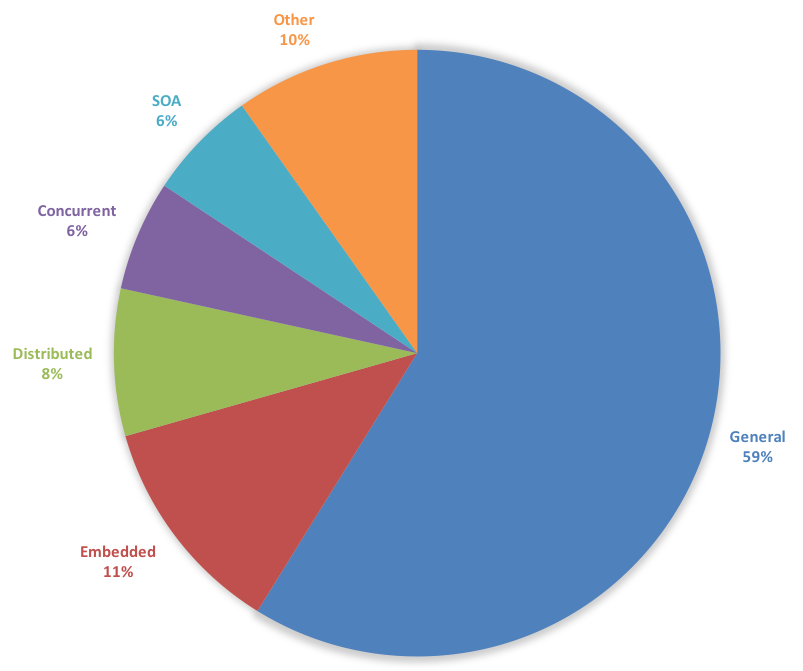
\includegraphics[width=0.6\textwidth]{Figures/litreview-adl-domains}
\caption{ADL Target Application Domain}
\label{figure:litreview-adl-domains}
\end{figure}

The analysis of the intended application domain of the languages can be found in \fref{figure:litreview-adl-domains}.  Interestingly very few of the languages were created for a specific business domain (e.g. financial analysis or industrial control systems) as over half the ADLs in the study do not explicitly target any business or technical application domain but are for general use.  There are a smaller number of ADLs specialised for embedded systems, distributed systems, highly concurrent systems and SOA, along with a number of individual ADLs for niche domains such as cyber-physical systems.

\begin{figure}
\centering
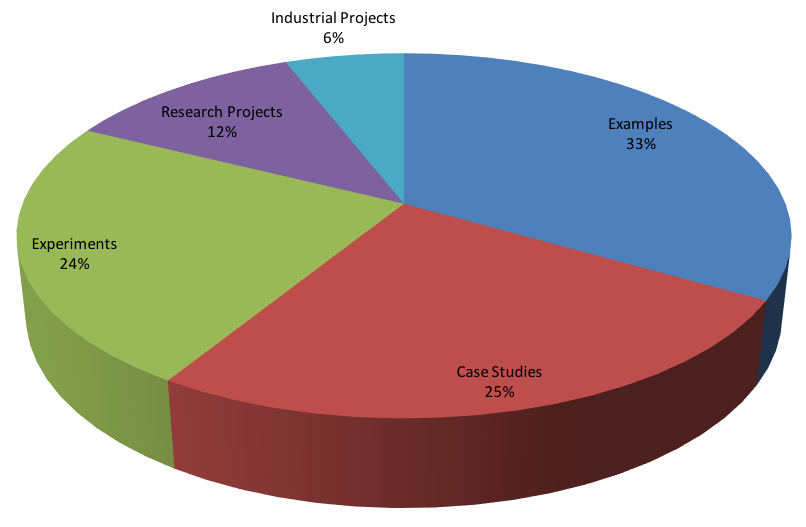
\includegraphics[width=0.6\textwidth]{Figures/litreview-adl-validation}
\caption{ADL Breadth of Application}
\label{figure:litreview-adl-validation}
\end{figure}

The analysis of the breadth of application of the languages can be found in \fref{figure:litreview-adl-validation}.  Unfortunately, as can be seen, less than 20\% of ADLs have been used beyond the case study level to perform significant research or industrial projects, suggesting a low degree of validation and practical experience with most of the languages.

The second area of interest to us were the \emph{architectural concepts} available in the different languages, to see if common industrial architectural concepts where in the languages or would need to be added.

The characteristics we analysed the ADLs for were the viewpoints that the ADL directly supports, the architectural concepts that they provide, whether they provide the ability to define behavioural semantics, whether they provide first class connectors and whether they provide first class architectural configuration constructs.  We chose to focus on these architectural concepts because of their wide use in the existing research literature and their general familiarity as concepts in industrial practice.

We were particularly interested in which viewpoints each ADL could support, as industrial architectural description nearly always needs a number of views to describe it, and the views supported provide a good insight into what the language can be used for.

None of the ADLs discuss a specific set of viewpoints that they define, so we analysed whether they provided effective support for the 6 viewpoints from \cite{rozanski2011-ssa2e} (which are Functional, Concurrency, Information, Development, Deployment and Operational).  We class a language has having first class connectors if the connector is defined separately to components and so is potentially reusable.  Similarly we consider architectural configuration to be a first class concept if it is described separately to the architectural elements and defines how they are combined, rather than being defined implicitly as part of the definition of the elements.

The complete data set for the architectural concepts available in each of the ADLs can be found in \tref{table:adl-concepts}.

The analysis of which viewpoints are supported by the different ADLs is presented in \fref{figure:litreview-adl-viewpoints}.

\begin{figure}
\centering
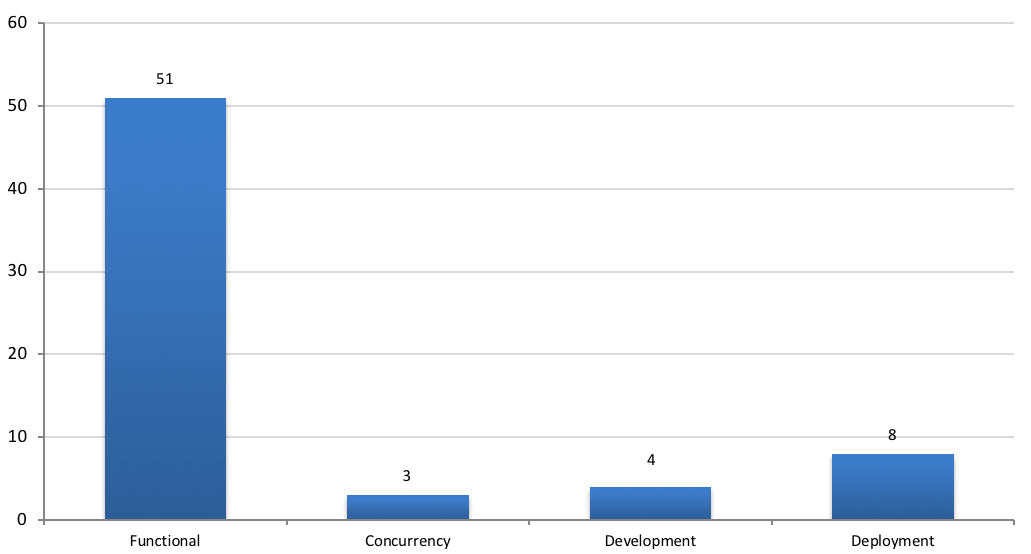
\includegraphics[width=0.75\textwidth]{Figures/litreview-adl-viewpoints}
\caption{Viewpoints Supported by ADLs}
\label{figure:litreview-adl-viewpoints}
\end{figure}

What is immediately evident from this analysis is that most ADLs only focus on the functional view of a system (i.e. its functional components and connectors and their organisation).  While clearly a key part of a system's architecture, most architects actually spend a lot of their effort working on other parts of an architecture (such as the deployment of the system).  So most of these ADLs are at best a partial solution to the problem of industrial architectural description.

\begin{figure}
\centering
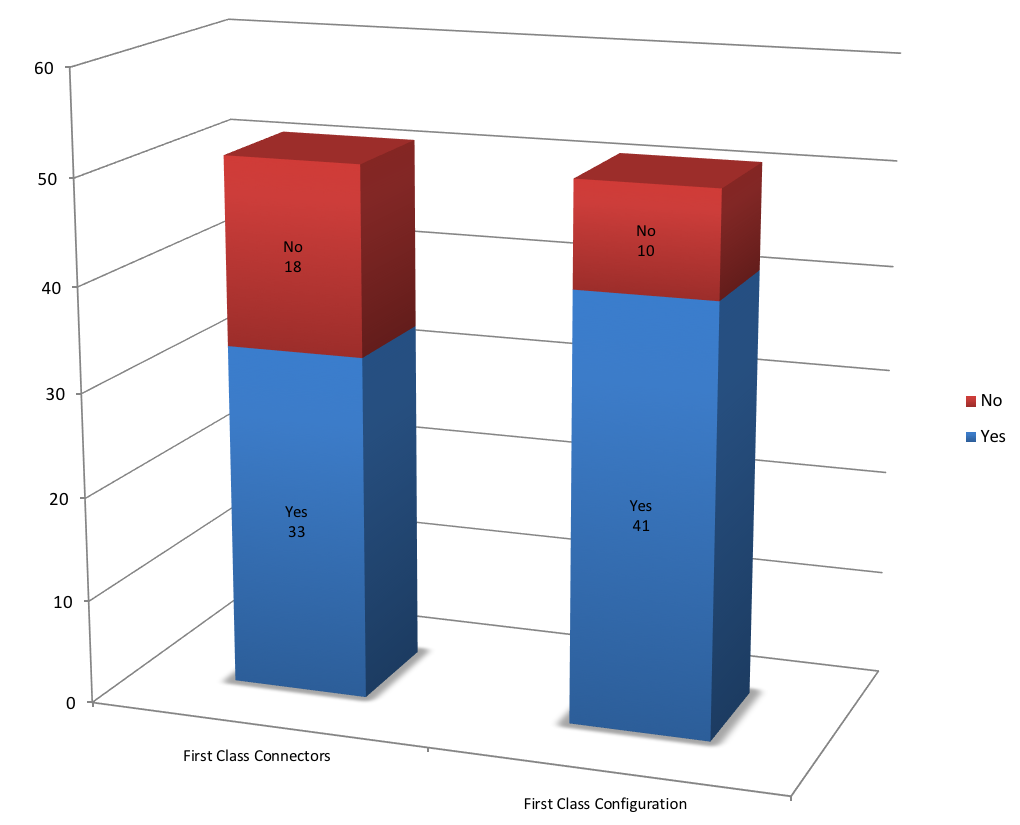
\includegraphics[width=0.75\textwidth]{Figures/litreview-adl-candc}
\caption{Connector and Configuration Support}
\label{figure:litreview-adl-candc}
\end{figure}

The analysis of the number of ADLs that provide support for first class connectors and architectural configuration as a first class concept is shown in \fref{figure:litreview-adl-candc}.

This analysis reveals a very positive result, as the clear majority of ADLs in the study provide some form of first class configuration, while less, but still nearly two thirds, provide support for first class connectors, which are both possible motivating factors for architects to use ADLs as existing informal and semi-formal notations tend not to support these concepts directly.

The third area of interest to us were the \emph{language mechanisms} available in the different languages, to assess the languages to see whether they could address common challenges (such as structuring and evolution) for large industrial architectural descriptions.

The attributes of the language that we analysed the literature for were as follows:
\begin{description} 
	\item[Structuring] - what mechanisms are available for structuring a large architectural description?
	\item[Evolution] - what mechanisms are provided to allow an architect to evolve an architectural description?  (Such as the ability to describe architectural variations, the ability to version all or parts of the description or support for dynamic architectures).
	\item[Qualities] - how provided or required architectural properties can be captured in the architectural description (e.g. properties, attributes, related models etc.).
	\item[Syntax] - what concrete syntaxes are available to capture architectural descriptions in the language?
	\item[Analysis] - how analysis of an architectural description could be supported using the language and any supporting technologies associated with it.
	\item[Tools] - what maturity are the tools that have been created to support the language? This can be "none", "prototype" (meaning an initial tool implementation applied to small problems), "research" (meaning a fully implemented tool applied to realistic problems by researchers), and "commercial" meaning that one or more tools have been implemented and used in an industrial context by people other than the tool's creators.
\end{description}

\begin{figure}
\centering
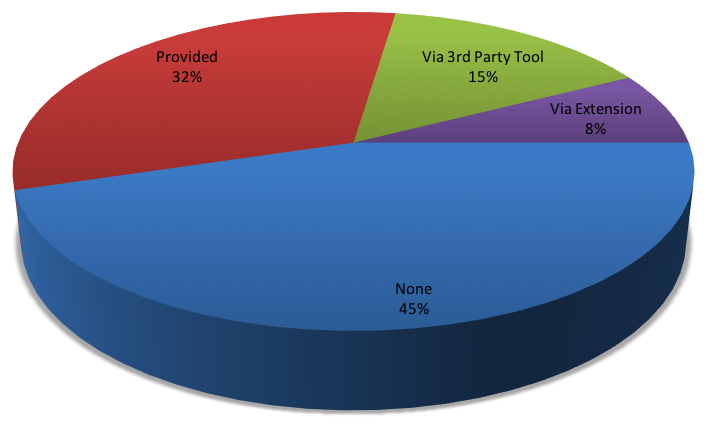
\includegraphics[width=0.6\textwidth]{Figures/litreview-adl-analysis}
\caption{ADL Support for Architectural Analysis}
\label{figure:litreview-adl-analysis}
\end{figure}

A common justification for using ADLs is the ability to perform automated analysis on the architectural description once it is represented using an ADL.  Therefore, we were interested to understand how many ADLs provided some sort of direct support for analysis of architectural descriptions.  

When we performed this analysis, we found that it was quite difficult because the analysis capabilities depend on support tools as much as the language and different ADLs provide quite different types of analysis capabilities.  To allow us to answer the question, we have defined four types of analysis capability:
\begin{description}
	\item [Provided] - where the ADL has specific support in the language to capture the data necessary to allow an automated tool to use it for analysis and explicit consideration has been given to making this possible.
	\item[Via Extension] - where the ADL has been designed such that its extension mechanisms could be used directly to support automated analysis via a tool.
	\item[Via 3rd Party Tool] - which means that the ADL provides some generic facilities that could allow a 3rd party tool to perform automated analysis, but where no explicit support for it is provided.
	\item[None] - where the language does not appear to be amenable to automated analysis.
\end{description}

This analysis is presented in \fref{figure:litreview-adl-analysis}.  As can be seen, less than half of the languages appear to provide realistic possibilities for automated analysis (and of course of those that do, many do not have working tools available for them).  We conclude therefore that automated analysis is only of interest in a subset of research groups working on ADLs.  A concern that we have with this situation is that an important motivator for adopting ADLs does not appear to be addressed in many of the ADLs that have been created.

\begin{figure}
\centering
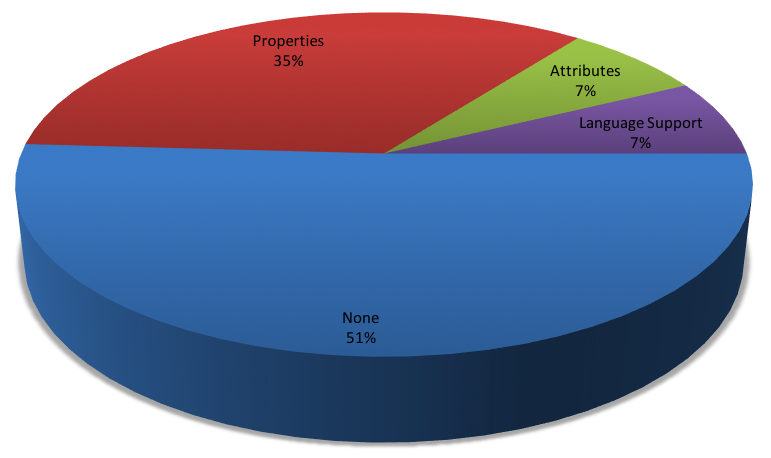
\includegraphics[width=0.6\textwidth]{Figures/litreview-adl-qualities}
\caption{ADL Support for Capturing System Qualities}
\label{figure:litreview-adl-qualities}
\end{figure}

A key goal of software architecture is to ensure that a system achieves the set of quality properties required for it to be successful.  This lead us to expect that ADLs would provide strong support for quality properties and we were interested in the types of mechanism used to represent them.  Having read the literature, we discovered that there were three broad levels of support for capturing quality properties in an architectural description:
\begin{description}
	\item[Properties] - where a generalised mechanism of (possibly typed) name/value pairs was available in the language and could be used to capture non-functional requirements and qualities but is not specifically provided for that purpose.
	\item[Attributes] - where specific pre-defined attributes relating to specific qualities (such as "transactions per second" for performance or "max connections" for scalability) can be captured within the language framework.
	\item[Language Support] - the case where languages provide a specific mechanism within the language for capturing quality requirements and capabilities (such as capturing security mechanisms and goals as first class language elements or providing a general purpose QoS or quality requirements sublanguage).
\end{description}

\fref{figure:litreview-adl-qualities} presents our analysis of this aspect of the capability of the ADLs.  It shows clearly that half of the languages provide no support for capturing system qualities, but that about a third (35\%) do have a generic properties mechanism which could be used to capture quality related information.  A much smaller number provide the ability to capture specific attributes (7\%) or have quality property features in their language (8\%).

\begin{figure}
\centering
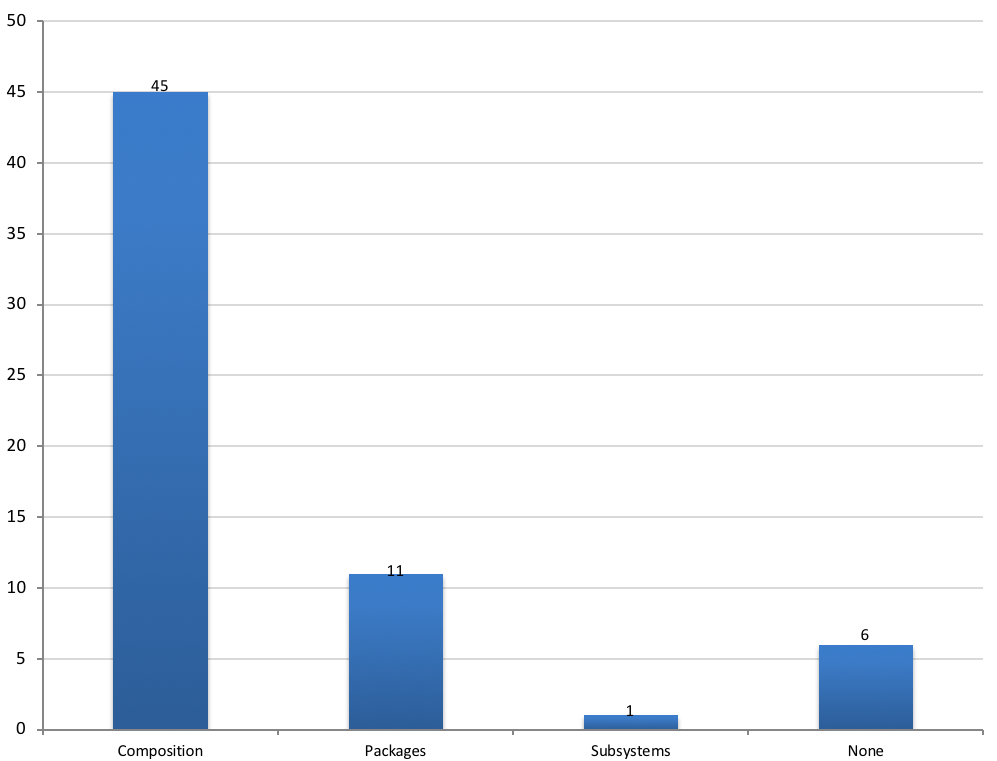
\includegraphics[width=0.75\textwidth]{Figures/litreview-adl-structuring}
\caption{Support for Structuring Architectural Descriptions}
\label{figure:litreview-adl-structuring}
\end{figure}

Many industrial systems are large, much larger than any case study or prototype experiment in the research domain.  A typical industrial system today can contain 500,000 to 1mm lines of code and dozens to hundreds of architectural elements.  Such systems cannot be described using languages that do not have effective structuring mechanisms to allow a system description to be broken down into smaller discrete parts.  This led us to investigate the mechanisms that each of the ADLs in the study provided for structuring the architectural description.  This analysis is shown in \fref{figure:litreview-adl-structuring}.

While a few of the ADLs (about 12\%) don't provide a structuring mechanism, most do, with nearly all of them offering \emph{composition} and a few offering \emph{packages} or \emph{subsystems} (in most cases in addition to composition - hence the total of values in the chart is larger than the number of ADLs in the study).
This is an interesting result, suggesting that most ADLs can be structured for large architectural descriptions, but that most of them utilise composition as the mechanism to achieve this, rather than providing a separate structuring mechanism like packages or subsystems.  This may imply restrictions in the flexibility of the structuring facilities available in those languages where only composition is available.

\begin{figure}
\centering
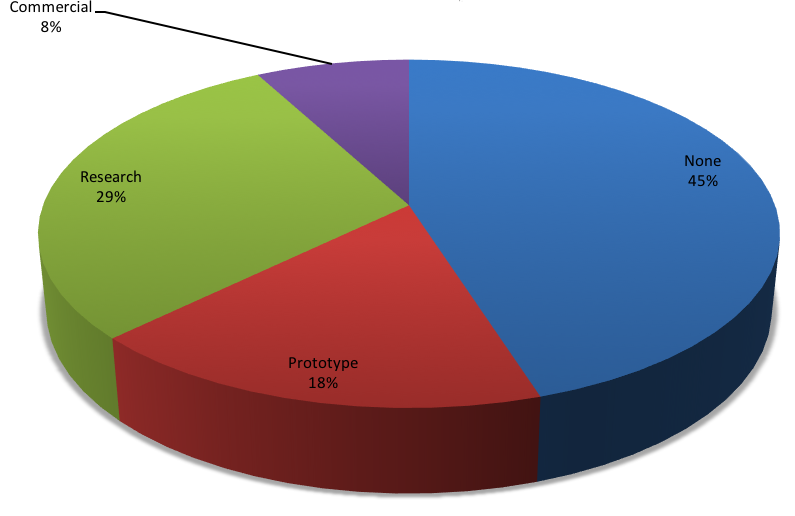
\includegraphics[width=0.6\textwidth]{Figures/litreview-adl-toolsupport}
\caption{Tool Support Available for ADLs}
\label{figure:litreview-adl-toolsupport}
\end{figure}

ADLs are often developed in conjunction with supporting tools to help architects to use them, which makes them more attractive for use on significant projects. \fref{figure:litreview-adl-toolsupport} presents our analysis of this feature of the ADLs in the study.

As can be seen, a very small percentage of the ADLs have commercially proven tools available to them, while about a third of them have tooling being used on research projects.  Nearly two thirds of the ADLs in our study provided no effective tool support.

\subsection{Conclusions}

\begin{description}
\item[ADL.RQ1] \emph{Which architectural viewpoints does each ADL support?}
All the ADLs in the study can represent functional views of the system and most of them only provide support for this view, but a small number of them allow deployment, concurrency or development views to be created too. Hence we conclude that the focus of most ADL research groups is how to represent the system's functional structure. This isn't surprising given how central a functional view is for most systems, but given the general acknowledgement of the importance of other viewpoints \cite{bachmann2011-documenting, brown2018-sad, kruchten1995-4plus1, rozanski2011-ssa2e} it does suggest that most of the existing ADLs will not be a complete solution to the problem of representing a software architecture.

\item[ADL.RQ2] \emph{Does the ADL provide structuring mechanisms for large ADs?}
Most ADLs in this study (45) provide the ability to structure a large architectural description by allowing composition of architectural elements (of course composition can also be used for other purposes, such as information hiding).   A smaller number provide specific mechanisms for structuring such as packages (11) and subsystems (1).  A few ADLs, surprisingly, do not appear to provide a structuring mechanism (6).  Some of the languages provide more than one mechanism that can be used to structure an AD (e.g. packages and composition) and this is why the numbers above sum to more than the number of ADLs in the study.\\
It is encouraging that most of the ADLs we surveyed provide at least basic facilities for structuring a large architectural description. This suggests that serious consideration has been given to the use of the ADL for realistic problems.  Those languages that don't allow structuring are presumably in an early stage of development or are not intended for industrial use.

\item[ADL.RQ3] \emph{Does the ADL support the analysis of an architecture?}
We found that about half of the ADLs (24 or 45\%) do not appear to allow a realistic option for automated analysis of architectural descriptions, which was something of a surprise to us.  Some of the languages do provide this though, with about 32\% of them providing direct support in the language, while 15\% allow this by providing mechanisms for 3rd party tools to embed information in the architectural description and 8\% allow for analysis by providing an extension mechanism that could allow analysis information to be added to an architectural description. \\
A clear motivation for capturing and maintaining an architectural description is the ability to gain useful and reliable automated analysis that can provide insight into the design that is otherwise difficult to obtain.  The fact that many ADLs being developed do not appear to provide analysis capabilities suggests that the problem of how to motivate others to use the language is often not part of the research process.

\item[ADL.RQ4] \emph{Can system qualities or quality requirements be captured in the ADL?}
Quality properties are central to the role and activities of the software architect and so we hoped for strong support for capturing qualities and quality requirements in the ADLs.  In fact, we found that more than half of the ADLs studied (28) do not appear to offer a facility to capture qualities and of those that do, most of them just provide a generic "properties" mechanism which can be used for a range of purposes including capturing qualities.  Only about 7\% of the languages provide quality property specific attributes in the language or include the ability to describe qualities as first class elements of the language.  This is a surprising situation, if the ADLs are expected to be used in an industrial setting.  Years of practical experience have taught us that achieving quality properties is a key objective of a software architect \cite{brown2018-sad, rozanski2011-ssa2e}, so we would have expected that supporting quality properties would have been an important requirement for an ADL.

\item[ADL.RQ5] \emph{Were prototype or production quality tools developed with the ADL?}
Given the importance of tool support in achieving adoption of new software technologies, we were surprised to find that 45\% of the ADLs in this survey do not appear to offer tool support that is ready for widespread transfer to industry and use.  29\% of the ADLs provide a tool that has been used for a research problem, and only 8\% of the ADLs have an associated tool that has been tested in an industrial context.\\
An important factor in applying ADLs on industrial projects is good tool support, preferably through extending tools that industry uses already.  In fact, we would go so far as to suggest that industrial adoption of any ADL without practical tool support is unlikely.

\item[ADL.RQ6] \emph{Has the ADL been applied to non-trivial problems outside the group of people who created it?}
Given the effort required to develop ADLs, we assume that most of them are intended for eventual technology transfer to industry.  Assuming so, the current degree of transfer out of the research groups is disappointing.  We found that 58\% of the ADLs have only been used by their creators, to create simple examples or experiments.  Another 26\% of the languages have only been used for case studies, again by their creators.  12\% appear to have been used for research projects, outside the creating group, while a mere 6\% of the languages have been applied in an industrial context. \\
It is our opinion that a technology can only be considered have had an impact when it is used by people other than its creators, and when considering the products of research groups, this means significant usage outside the originating research group and ideally in an industrial context.  Nearly all the ADLs we have surveyed fail this test, with less than 20\% of them having been used outside their originating group (based on the publications we could find).  It is possible that some of these ADLs have been used industrially but the case studies not published, however we feel that this is unlikely given the positive impact that publishing such case studies would have.  We believe that this finding in itself is cause for reflection within the ADL research community (as was the previous similar finding from a workshop some years ago \cite{woodshilliard2005-adlsinpractice}).
\end{description}

\section{Prioritisation of Architectural Effort}
\label{section:litreview-prioritisation}

An observation we have made from software architecture practice is that the prioritisation of an architect's activity is a complex process, with many factors being taken into account. The software architect had broad responsibilities on a project and they can be involved in almost any technical aspect of a project at some point in its lifecycle. This can make it difficult for an architect to prioritise their effort in such a way that they have the time available to prioritise quality properties like energy efficiency that are often not explicity prioritised by many of the system's stakeholders (we've observed that similar problems often occur with security, performance and scalability properties).

This situation led to our second research question \emph{RQ2 - How can architects prioritise their attention on energy efficiency?}

We do not observe role-specific heuristics or techniques in common use in industry and so were interested in whether there were approaches in the research literature which could be taught to new architects to allow us to further our goal of making it easier for software architects to address energy efficiency as an architectural concern.  

We were aware of generic time management techniques (like \cite{allen2015-gettingthingsdone} and \cite{koch1998-8020principle}) but we wanted to provide more tailored and prescriptive advice, specific to software architects, rather than more general advice of the sort found in these techniques.

We were also already aware of an entire architectural method, called Risk and Cost Driven Architecture (RCDA), designed by Eltjo Poort \cite{poort2012-rcda}, which guides software architects to focus their attention is using risks and costs.  This method transforms the architect's approach from defining finished architectural structures at the start of a project, to working throughout the project to provide a stream of decisions, using the risk and cost of open decisions to prioritise the architect's work. It can certainly help architects to focus attention on their most important concerns and might well lead architects to consider energy efficiency more often if it was widely applied.  However we know that RCDA is not very widely applied across the industry and so we were interested in whether there were simpler approaches that required less commitment to adopt.

\subsection{Research Methodology}

We identified the research literature to include in the study by searching commonly used literature catalogues as well as manually inspecting the reference lists of relevant papers and following other relevant references found.

After some experimentation we defined our search query for online catalogues to be \emph{("software architect" or "software architecture") AND ("prioritize" OR "prioritisation" OR "focus") AND ("attention" or "effort")}.  The syntax of the query had to be refined for different catalogues as they provide different search facilities, but this was a simple matter of performing multiple simpler queries against them.

We searched key online literature catalogues for papers that matched our query in in their title, abstract or keywords.  The four catalogues we used were the ACM Digital Library (advanced search), Google Scholar, IEEEXplore and Microsoft Academic Search.

The different catalogues returned different result sets for the query, with ACM Digital Library returning 11 results, IEEEXplore 12, Google Scholar nearly 80 and Microsoft Academic Search 12.

We then consolidated these results, by concatenating and removing duplicates from the ACM and IEEE results and manually scanning the results from Google Scholar to identify studies which suggested some aspect of prioritisation in their title (which resulted in 6 additional unique entries).  Finally, Microsoft Academic Search returned relatively few entries and most were obviously not relevant to our search, but 4 additional items were added manually from this source.

When we inspected the results, it became obvious that there was a significant body of literature on the subject of prioritising system quality requirements.  This is not exactly what we ask in our research question, which is more general, but we judged that such approaches might provide answers to the question, so we investigated them further.  A manual process of reference following and additional searches revealed that many of the studies in this area have little or no consideration of industrial usage or validation.  However we did find some that appeared to have potential industrial relevance and this resulted in another 20 studies which had not been returned by our search query but we believe are representative of this research area.

At this point we had a list of 46 candidate studies for consideration.

To narrow the list to the most relevant for our needs, we identified the following criteria for inclusion in our survey.

\begin{description}
	\item[IC1] The study has been peer reviewed and is at least 2500 words long.
	\item[IC2] The study addresses some aspect of how architects prioritise their effort and attention (rather than just decision making for example).
	\item[IC3] The advice, technique(s) or approach(s) in the study can be applied by an industrial software architect.  (For example, they have some industrial validation and do not rely on a research tool or technique).
	\item[IC4] For practical reasons the study must be written in English.
\end{description}

When we applied inclusion criterion IC1, this removed 5 items from the list and applying IC2 (to focus on architectural effort prioritisation) left 13 for consideration.  When we applied IC3, to ensure industrial applicability, this left 6 studies, due to the others not having any industrial validation.  All of the studies we considered were written in English so IC4 was unnecessary.

\subsection{Analysis of the Results}

In his paper \emph{} \cite{kruchten2008-architectsdo}, Kruchten recommends a prioritisation of effort into 50\% architecting (design, validation, prototyping, documenting), 25\% getting input (from users, for requirements, on technology) and 25\% providing information (communicating the architecture, assisting stakeholders). The recommendation comes from experience in managing a 10 person architecture team in the early 1990s.  To support his theory, he shows how other time allocations can cause architectural (behavioural) anti-patterns.  This is anecdotal rather than empirically-based advice, but is based on large scale industrial experience.  It does not help the architect to know where to focus but is clear advice on the types of activities to focus their attention and the amount of time to spend on each.

In their paper \emph{Decision-making techniques for software architecture design: A comparative survey} \cite{falessi2011-archdecisionsurvey}, Falessi et al report a survey of the decision making techniques in academic literature.  This is only partly related to prioritisation but it was one factor in their study.  They found that the priority of a quality attribute chould be defined by direct weighting by stakeholders, an elicited weight which involves "decomposing a multiple-criteria decision-making problem into a quality attribute hierarchy" (and they note the significant effort involved in this) or using a utility curve (which again is significant effort).  However their results are inconclusive, reporting that "no decision-making technique is more (or less) susceptible than any other technique to the entire set of difficulties taken into account in this study, that is, no decision-making technique dominates (is always better than) any other one".  Therefore there is little concrete advice for the software architecture practitioner to take from this study.

Another survey paper is \emph{Mature architecting-a survey about the reasoning process of professional architects} \cite{vanheesch2011-maturearch} by van Heesch and Avgeriou, which reports the results of a survey of 53 industrial software architects to find out how they reason during decision making.  Prioritisation was part of the study scope by the only prioritisation insights in the results were   
that "the quality attribute requirements are clearly found more important than the functional requirements" and "requirements should be prioritized; the most important ones and the ones that are hardest to fulfil should be regarded first, as they bare potential risks" (sic).  These insights sound like good advice, but don't provide a significant degree of guidance to an architect focus attention in a particular way.

The industrial study \emph{Prioritization of quality requirements: State of practice in eleven companies} \cite{svensson2011-qrprioritisation} by Svensson et al reports on a study of architects in 11 industrial companies to find out how they prioritise their system quality requirements.  Representative techiques that they suggest are Numerical Assignment (Grouping), Pair-Wise Comparison, Cost-value approach, Cumulative voting (\$100-Dollar Test) and Ranking.  They had three main findings, that (1) ad-hoc and grouping (numerical assignment) of requirements are the dominant methods for prioritizing quality requirements; (2) although numerical assignment is used frequently in quality requirement prioritization, quality requirements are by default often considered to have the lowest priority; and (3) the reasons for not prioritizing quality requirements was not related to the prioritization process itself, but rather how quality requirements were treated in the overall requirements engineering process.  They also found that It is most common to have no specific or explicit criterion defined when prioritizing quality requirements.  So for the architecture practitioner, one useful finding is that ad-hoc and grouping are used to prioritise quality requirements - these are techniques that industrial architects could easily apply.  And some comfort can be taken from the second finding about the difficultly of prioritising quality requirements - it is a common problem in many environments.

Another study focusing on quality requirements is \emph{Can we know upfront how to prioritize quality requirements?} \cite{fernandez2015-qrprioritisation} by Condori-Fernandez and Lago.  The context of this study is service design for smart transport systems and involved studying a group of postgraduate students solving a service design problem set by an industrial partner company.  The study aimed to identify which quality requirements are most important from the software architect's viewpoint and which are most stable over the service design process.  The study does investigate the prioritisation decisions made, it doesn't ask how they are made, so does not significantly contribute towards answering our question.  The main prioritisation conclusion was that "the design space specification phase of our service design method can play a crucial role in QR prioritization", which is not a generally usable result for most architects.

Finally in the recent study \emph{An industry experience report on managing product quality requirements in a large organization} \cite{mohagheghi2017-managingqr}, Mohagheghi and Aparicio report their experience in managing quality requirements in a Norwegian goverment department's large agile development programmes.  There isn't much discussion of prioritisation of the quality requirements in the study with the only significant insight being that stakeholder workshops were necessary to prioritise quality requirements.  However there isn't any information on how the architects focused their effort during the process.

\subsection{Conclusions}

From a large body of research literature in the area of architectural prioritisation and particularly prioritisation of quality requirements, we found that very little of it is directly applicable to an industrial practitioner as much of it is speculative, theoretical or unvalidated.  Of the literature we found that was of potential value, we have an experience-based view of the amount of time the architect should spend on different activities (Kruchten) and an industrial survey result that most prioritisation is ad-hoc or based on simple (numerical) grouping of requirements (Svensson et al).  This falls some way short of the amount of guidance that we had hoped to be able to provide to an architecture practitioner.  We will return to this topic in \cref{chapter:prioritisation} to consider what further guidance could be provided on this topic.


\section{Architectural Guidance for Energy Efficiency}
\label{section:litreview-energyguidance}


As awareness of power usage and the need for improved energy efficiency grows across the ICT sector, attention is turning from an initial focus on data centre efficiency \cite{delforge2014-datacentreenergy} to how the software applications running within them can contribute to a reduction in net energy consumption.  Yet a previous survey of software architecture practitioners \cite{bashroush2016-datacentreenergy} has revealed both a growing awareness of the need to treat energy efficiency as a first class concern and also a lack of tangible advice and guidance on how to achieve this.

Our goal is to raise awareness of energy as an architectural concern with software architecture practitioners and so we wanted to investigate whether there was existing research which had resulted in practical advice that software architects could use to address energy as a property of their systems.

This survey of the research literature partly addresses research question \emph{RQ3 -  What design guidelines can we provide to guide architects to improve energy efficiency of their systems?}.

\subsection{Research Methodology}

We identified the research literature to include in the study by searching commonly used literature catalogues as well as manually inspecting the reference lists of relevant papers and following other relevant references found.

After some experimentation we defined our search query for online catalogues to be \emph{"software architecture" AND "(energy OR power) (consumption OR efficiency)" AND (principles or tactics)}.  The syntax of the query had to be refined for different catalogues as they provide different search facilities, but this was a simple matter of performing multiple simpler queries against them.

We searched key online literature catalogues for papers that matched our query in in their title, abstract or keywords.  The four catalogues we used were the ACM Digital Library (advanced search), Google Scholar, IEEEXplore and Microsoft Academic Search.

Predictably, the different catalogues returned very different results, with ACM Digital Library returning 95 results, IEEEXplore 63, Google Scholar nearly 3,000 and Microsoft Academic Search adding only 3 additional items.

We then consolidated these results, by concatenating and removing duplicates from the ACM and IEEE results and manually scanning the results from Google Scholar, adding any entries that had not been returned by the previous searches (which resulted in 16 additional unique entries, as well as confirmation of most of the entries returned by the ACM and IEEE searches).  Finally, Microsoft Academic Search returned relatively few entries and most were obviously not relevant to our search, but 3 additional items were added manually from this source.

From this list, we identified the most obviously relevant items (those with titles indicating energy related tactics or principles or architectural techniques) and found a small number of additional items that could be relevant, which were added to the list.

At this point we had a list of 182 candidate studies for consideration.

To narrow the list to the most relevant for our needs, we identified the following criteria for inclusion in our survey.

\begin{description}
	\item[IC1] The study has been peer reviewed and is at least 2500 words long.
	\item[IC2] The study addresses some aspect of energy efficiency as a quality property of a system.
	\item[IC3] The reference provides some tangible advice (such as a tactic, a design principle or a technique) which could be used to help address the energy qualities of a software system.
	\item[IC4] The advice provided by the study is relevant to addressing energy as an architectural concern (rather than, for example, code path optimisation).
	\item[IC5] The study is relevant to large scale enterprise applications such as those found in large end-user organisations, the products of software companies supplying them, or those applications found in Internet-oriented companies, such as SaaS software providers.
	\item[IC6] For practical reasons the study must be written in English.
\end{description}

When we applied inclusion criterion IC1, this removed two items from the list and applying IC2 (to focus on energy as a quality property) removed a large number of the studies, leaving 43 for consideration.  Of these 13, met the requirements of IC3 (to provide tangible advice) and 11 of them met the requirements of IC4 (i.e. they were architecturally relevant).  Finally, applying criterion IC5 resulted in the elimination of another two studies, leaving 9 to be analysed further.

Having identified the 9 references of interest, we analysed their content in order to allow further classification.  This proved to be a very straightforward process due to the small number of studies that met our inclusion criteria and very clear similarities between the references.  Our classification is summarised in \tref{table:archguidancestudies}.

\begin{table}
\caption{Classification of Architectural Guidance Studies}
\label{table:archguidancestudies}
\begin{center}
\begin{tabular}{| l | c | l |}
\hline

\textbf{Classification} & \textbf{Count} & \textbf{References} \\
\hline

Cloud Energy Efficiency Tactics & 4 & \cite{procaccianti2013-cloudenergyefficiency, procaccianti2014-greentactics, procaccianti2014-greentactics-wicsa, procaccianti2015-cloudenergy-litreview} \\
\hline

Cyber-Foraging Tactics & 2 & \cite{lewis2015-foragingtactics, lewis2016-foragingdm} \\
\hline

Energy Perspective & 2 & \cite{jagroep2015-energyperspective, jagroep2017-energyperspective} \\
\hline

Design Practices & 1 & \cite{procaccianti2016-twobestpractices} \\
\hline

\end{tabular}
\end{center}
\end{table}

Four of the references \cite{procaccianti2013-cloudenergyefficiency, procaccianti2014-greentactics-wicsa, procaccianti2015-cloudenergy-litreview} are all related to work performed at Vrije Universiteit in Amsterdam to investigate architectural tactics to address energy efficiency in cloud computing environments (so called "green architectural tactics").

Two of the references \cite{lewis2015-foragingtactics, lewis2016-foragingdm} are related to work on "cyber-foraging" (the process of allowing mobile devices to extend their computing power and storage by offloading computation or data to more powerful servers located in the cloud) performed at the Software Engineering Institute (SEI) at Carnegie Mellon University and  Vrije Universiteit in Amsterdam.

Two of the references \cite{jagroep2015-energyperspective, jagroep2017-energyperspective} are the result of research into treating energy efficiency as an architectural concern, performed at Utrecht University in the Netherlands, with the industrial software company Centric Netherlands BV.  This work led to the creation of an architectural perspective \cite{woods2005-perspectives} that provides guidance to a software architect in how to improve the energy characteristics of the system.

The last reference \cite{procaccianti2016-twobestpractices} is an empirical evaluation of the energy consumption impact of two specific architectural practices, again based on research from Vrije Universiteit in Amsterdam.

\subsection{Analysis of the Results}

The studies in the \emph{Cloud Energy Efficiency Tactics} set start with a literature review \cite{procaccianti2013-cloudenergyefficiency} that identifies three strategies for cloud energy efficiency, namely \emph{Energy Monitoring}, \emph{Self-Adaptation} and \emph{Cloud Federation}.  The study then identifies the components and techniques that have been proposed in the research literature to address cloud energy efficiency, within these three areas.  These components and techniques are not, in most cases, directly usable by an application architect, but are useful background knowledge for them.

The later papers in this group develop the work further to provide direct architectural guidance for practitioners in the shape of a set of architectural tactics that we summarise in \tref{table:cloudtactics}, using the tactic descriptions from the original reference.

\begin{small}
\begin{longtable}{| l | l | p{8cm} |}
\caption{Architectural Tactics for Cloud Energy Efficiency}
\label{table:cloudtactics}\\
\hline

\textbf{Strategy} & \textbf{Tactic} & \textbf{Description} \\
\hline

\multirow{3}{*}{Energy Monitoring} & Metering & The Metering tactic consists of collecting power metering information from the hardware through dedicated software components called energy collectors. Collectors are usually in a many-to-many relationship with physical power meters. These collectors share information via an energy communication bus (ECB) that provides a common interface for energy information. In addition, the energy consumption information is stored in a dedicated energy database that can have different levels of granularity. Finally, a GUI component called an "energy dashboard" provides graphical representations of energy information along with useful reporting for both cloud service providers and customers. \\ \cline{2-3}
& Static Classification & This tactic consists of classifying the different resources in terms of energy efficiency through the use of energy indicators. This classification is static, based on technical specifications and characteristics of the devices themselves rather than real-time information. \\ \cline{2-3}
& Modelling &  Modeling tactic enables a dynamic estimation of power consumption values through predictive energy models. These Models are embedded in energy indicators, similar to those in the Static Classification tactic. However, these energy indicators do not statically classify physical resources, but rather provide a dynamic estimation of the power consumption of the software components. Typically, energy models are built through regression analysis based on software runtime metrics (e.g. CPU, disk, memory). \\
\hline
\multirow{3}{*}{Self-Adaptation} & Scaling Down & This tactic reduces deployed IT resources when not required for current system load.  This tactic utilises the idea of a "scale unit" which is a pre-defined quantity of "IT resources" \cite{rogers2008-greenitpatterns} explicitly modeled as a software component. Modeling Scale Units is useful for planning the scaling operations because it defines a finite number of configurations for the VMs. Thus, it is possible to associate each configuration with a particular level of demand or system load. The Adaptation Engine is the component that performs the Scaling operation; this role is typically played by the Hypervisor. Another key component is the SLA Violation Checker to perform the checks required during scaling operations to ensure that service-level objectives are maintained at all times. \\ \cline{2-3}
& Consolidation & This tactic concentrates VM instances on the minimum number of servers needed, to allow unused servers to be powered down. The main component of the Consolidation tactic is the VM Allocator, the software component responsible for live VM migration, which is often part of the Hypervisor. The SLA Violation Checker is also needed as well to check that service-level objectives are maintained after VM migrations. \\ \cline{2-3}
& Workload Scheduling & This tactic is meant to prioritize and assign workload to the different virtual resources available in order to match demand. In this tactic, a Workload Scheduler is used to dispatch workloads to VMs. The Scheduler normally uses one or more queues to arrange the workloads. Queues can be differentiated in terms of priority levels, QoS requirements or deadlines. The SLA Violation Checker ensures that all service-level objectives are met. \\
\hline
\multirow{2}{*}{Cloud Federation} & Energy Brokering & This tactic makes energy information about services an additional parameter for service discovery and selection. It is realized by means of two components, an Energy Broker and a Green Service Directory (GSD). The Energy Broker enables access to energy-efficient services. It receives requests for cloud services that perform a specific task and returns a pointer to the most energy-efficient service available in the multi-cloud that can perform the requested task. In this, Energy Brokers make use of a GSD, which is a repository where all the cloud providers in the multi-cloud store the energy information of the services they provide. \\ \cline{2-3}
& Service Adaptation & The Service-Adaptation tactic describes how cloud platforms should switch to these more energy- efficient services.  It is realised by two components, the Energy Orchestator and the SLA Violation Checker.  The Energy Orchestrator communicates with the Energy Broker to discover energy-efficient services that fulfill a certain task and performs the registration of those services with the system. This operation is authorized by the SLA Violation Checker, which ensures that the new services meet the service-level objectives required by the system. \\
\hline

\end{longtable}
\end{small}

These tactics are clearly useful in the correct context and can guide architectural decisions that allow energy to be considered as a first class architectural concern.  However these tactics are primarily of use to an infrastructure architect or an application architect in an environment where they have a lot of control over he infrastructure environment and can make significant changes to it.  Our area of interest is application architects working in a more common situation where they have limited control over the fundamental workings of their infrastructure platform.

The papers in the \emph{Cyber-Foraging Tactics} group provide a practical set of tactics for solving architectural problems "...to enable mobile devices to extend their computing power and storage by offloading computation or data to more powerful servers located in the cloud or in single-hop proximity" \cite{lewis2015-foragingtactics} and develop these ideas to provide a decision model to allow the tactics to be used effectively.  This research has developed a sophisticated and extensive catalogue of tactics, comprising 10 functional tactics (with two further variants of them) and 12 non-functional tactics (with 6 further variants of them).  These tactics offer extensive architectural advice and can clearly have a dramatic impact on the energy usage of mobile applications in systems that implement them.  However these tactics are not generally applicable beyond the specific problem domain of cyber-foraging and so do not help us address our question of how to guide application software architects in considering the energy efficiency of their applications.

The studies in the \emph{Energy Perspective} group both define an architectural perspective (that is "a collection of activities, tactics, and guidelines that are used to ensure that a system exhibits a particular set of related quality properties that require consideration across a number of the systems architectural views" \cite{woods2005-perspectives}).  The perspective aims to standardise and organise the work of the architect in meeting energy efficiency goals for their system.  This includes identifying, testing and selecting architectural tactics to achieve particular goals which the architecture does not initially meet, and the perspective aims to provide a framework to guide and formalise this process.

The full definition of the perspective can be found in \cite{jagroep2017-energyperspective}, but to briefly summarise its key activities, it recommends the following steps in addressing energy as an architectural concern:

\begin{enumerate}
	\item \textbf{Capture energy requirements} - Energy requirements can be formulated like other requirements, however it might prove difficult to translate the requirements into quantitative goals. Cross-checking the goals with stakeholders is essential to ensure the software will fulfill the requirements.
	\item \textbf{Create energy profile} - An energy profile of the software provides the stakeholder with an objective starting point and benchmark to identify "hot spots" and determine whether the desired results have been achieved. Creating the profile requires energy consumption and performance measurements and can be visualized by creating an overlay for the architectural description.
	\item \textbf{Assess against requirements} - Using the energy profile an assessment should be performed on whether the software meets the requirements and if not, the assessment should show what quantitative goals are not met and the (software) aspects that are directly related to these goals.
	\item \textbf{Determine adjustments} - If required, adjustments should be determined to meet the requirements. Tactics, patterns and other known solutions should be considered that affect specific "hot spots" signaled by the quality measure.
	\item \textbf{Apply adjustments} - Adjustments related to infrastructure can often be applied immediately by an administrator with little effort. Changing the software may be significant effort and disrupt other software delivery. The resources required to apply an adjustments should be included in the business case for the adjustment.
	\item \textbf{Evaluate adjustments} - Determine that requirements are met without unwanted side-effects. Requires measurement in the newly environment and comparison against the energy profile. Relevant stakeholders need to judge whether the results are satisfactory.
\end{enumerate}

As with most perspectives, the process is an iterative one, performing these steps repeatedly as the architect's knowledge of the situation increases and the architecture is changed in response to the process.

The authors of the perspective suggest considering the cloud energy efficiency tactics that we reviewed earlier in this survey along with the tactics of \emph{Increasing Modularity}, \emph{Optimising Network Load}, \emph{Increase Hardware Utilisation}, \emph{Concurrency Architecture Variations}.

The architectural perspective appears to be a valuable artefact for an architecture practitioner and would provide them with significant assistance in understanding how to treat energy efficiency as an architectural concern.  The weakest part of the perspective at present is the set of tactics, which are quite general and would be more valuable if they were based on industrial case studies.  We return to this point in \cref{chapter:energydesignprinciples}.

Finally, the paper classified as \emph{Design Practices} is an empirical evaluation of the energy impact of two well known design practices, namely to \emph{Use Efficient Queries} and to \emph{Put Applications to Sleep}.  

The study reports a research exercise that ran two experiments.  The first experiment ran inefficient MySQL queries (SQL relational database queries) and compared the energy usage of the scenario to the same functional scenario using an efficient database query.  The second tested two versions of the Apache web server, firstly the standard version, which calls the operating system \emph{sleep} function when it is idle, and one with all calls to the operating system \emph{sleep} function removed.  The same workload was applied to both versions of the server and the resource utilisation and energy consumption of each measured.  The study ran the experiments in a specific controlled environment to allow interference free measurements of resource utilisation and physical power consumption.

The results of the study were unsurprising with the use of an efficient query significantly reducing the machine resources required to process the scenario resulting in a 25\% energy saving.  Similarly, putting the application to sleep had a measureable and repeatable, but smaller, impact on energy consumption (14\%).

This study provides a useful result to validate two simple design practices which have been proven to reduce energy consumption as a result of the study.  However, the design practices are at a fairly detailed level and are unlikely to result in significant architectural decisions.  So while of interest to a software architecture practitioner, this study does not provide a significant amount of guidance on how to start improving the energy characteristics of their applications.

\subsection{Conclusions}

Our research question, RQ3, asked "What design guidelines can we provide to guide architects to improve energy efficiency of their systems?"  Our answer, from a  review of the relevant research literature, is that the practice of treating energy efficiency as an architectural concern is still immature and more assistance is needed for the industrial practitioner.  The most promising, generally applicable and currently valuable advice available can be found in the Energy Architectural Perspective defined at Utrecht University and Centric Netherlands BV.  This perspective provides a clear and useful approach to guide the architect in addressing energy as an architectural concern.  The weakest part of the perspective is the set of architectural tactics that it has to refer to.  We partly address this concern in \cref{chapter:energydesignprinciples}.

Other advice for the practitioner is available in the other studies, and is of value in the correct context, particularly for those implementing cyber-foraging systems or designing cloud based infrastructure to be energy efficient, or those application architects able to design their infrastructure platforms.

\section{Application Energy Consumption Analysis} \label{sec:litreviewenergy}

As we noted earlier, the energy usage of information and communications technology (ICT) systems is starting to receive significant attention due to the sharply increasing demand for electricity to run the large number of data centres that exist today.

Significant research has been undertaken to understand the nature of the energy demand of ICT systems and significant progress has been made in a number of areas.  At the data centre level, there is now a fairly good understanding of how data centres use power and some understanding of how to reduce the amount of power required in the data centre environment \cite{dc4cities2014_dcmetrics, dayarathna2016-dcenergy}.  At the micro-level, there have been some promising steps in understanding how individual programs consume power, to the point where it is possible to quite accurately predict and compare the power consumption of different options for program implementation under laboratory conditions \cite{bourdon2013-powerapi, noureddine2012-hotspots, islam2016-energysoftwarefeatures, acar2016-beyondcpu}.

The problem for the software architect is that their interest sits between these two extremes as they need to understand the energy consumption at the overall application level rather than at the individual software module level or at the data centre level where many applications are consolidated.  In particular, they really need to understand the energy characteristics of different usage scenarios of their applications so that they can compare them and use this information when making architectural tradeoffs.

This situation was the reason for our fourth research question, which was \emph{
RQ4 - How can we make architects aware of the runtime energy characteristics of their applications?}

In order to start answering this research question, we decided to perform a survey of the relevant research literature in order to understand what research had already been performed in the area of application level runtime energy usage monitoring.

\subsection{Research Methodology}

We identified the research literature to include in the study by searching commonly used literature catalogues as well as manually inspecting the reference lists of relevant papers and following other relevant references found.

After some experimentation we defined our search query for online catalogues to be \emph{(software) AND (predicting OR measuring) AND (energy consumption) AND NOT (android or mobile) AND NOT sensor}.  The syntax of the query had to be refined for each catalogue as they provide different search facilities, but this was a simple matter of restating the query as multiple simpler queries in most cases.

We searched key online literature catalogues for papers that matched our query in their title, abstract or keywords.  The four catalogues we used were the ACM Digital Library (advanced search), Google Scholar, IEEEXplore and Microsoft Academic Search.

The different catalogues returned different sets of results, with ACM Digital Library returning 1216 results, which had to be manually inspected to extract the ones relevant to computing (to exclude, for example, references about energy management for buildings) which resulted in 24 studies of interest.  IEEEXplore returned 31, Google Scholar returned 90 results and Microsoft Academic Search returned 84 results on a wide range of subjects, which, when manually inspected added 3 more relevant items.

We then consolidated these results by concatenating the result sets and removing duplicates from the list.

We identified the most obviously relevant studies in our candidate list (those with titles indicating work directly in the area of application energy monitoring) and scanned their reference lists for other relevant studies, which added a further 14 entries.

At this point we had a list of 79 candidate studies for consideration.

To narrow the list to the most relevant for our needs, we identified the following criteria for inclusion in and exclusion from our survey.  IC1 - IC3 are the inclusion criteria and EC1 and EC2 are the exclusion criteria.  To be included in the survey a study had to meet all of the inclusion criteria and not meet any of the exclusion criteria.

\begin{description}
	\item[IC1] The study has been peer reviewed and is at least 2500 words long.
	\item[IC2] The study describes an approach, technique or technology for runtime monitoring of the energy usage of application software.
	\item[IC3] The study is relevant to large scale enterprise applications such as those found in large end-user organisations, the products of software companies supplying them, or those applications found in Internet-oriented companies, such as SaaS software providers.
	\item[EC1] The study will be excluded if only relevant to mobile device technology or hardware (such as processor chips or sensors).
	\item[EC2] For practical reasons the study will be excluded if not written in English.
\end{description}

When we applied inclusion criterion IC1, which eliminated on study and IC2 (that the study must be about runtime monitoring of application software) then reduced the list to 31 items.  Applying IC3 (to ensure that the approach could be applied to an enterprise system) reduced the list to 19 items and applying EC1 to eliminate approaches that were only relevant for mobile or hardware devices left 13 to be analysed further.  All of our candidate studies were written in English so EC2 did not apply.

Having identified the 13 references of interest, we analysed their content in order to allow further classification.  

\subsection{Analysis of the Results}

The 13 references comprised 1 survey paper, 2 case studies and 10 papers describing energy monitoring tools of some sort.

The survey paper \emph{A Review of Energy Measurement Approaches} by Noureddine et al \cite{noureddine2013-energyreview} was a useful additional survey of the area and usefully summarised the approaches found in this area a few years ago (which based on our survey do not appear to have changed materially).  They found that there are \emph{model based}  approaches and \emph{measurement based} tools.  They found three primary model based approaches: cost based models, models implemented in middleware systems and models based on measured server workload.  They also found three primary measurement based tools: PowerScope that maps physical energy measurements to processes and program structures; pTop from the Linux operating system, which  
creates energy estimates for processes using resource utilisation profiles gathered by a kernel module; and PowerAPI and Jalen, the author's own tools that estimate power consumption for processes using operating system statistics and power readings and allocate power consumption to the elements of the software executed via the tools.  This paper helped to provide some context for understanding this area, but is an incomplete survey and does not aim to provide information for the architect to use directly.

The two case studies were \emph{Software Energy Profiling: Comparing Releases of a Software Product} by Jagroep et al \cite{jagroep2016-comparingreleases} and the much smaller \emph{Unit Testing of Energy Consumption of Software Libraries} by Noureddine et al \cite{noureddine2014-energyutest}.  Both of these case studies show how energy concerns can be integrated into the project lifecycle.

Jagroep et al reports on a significant research project performed in conjunction with an industrial company, to measure and compare the energy consumption of a commercial document generation system product, over a series of releases.  They used both hardware and software energy measurement tools to measure energy consumption of the product during specific usage scenarios each time the product was being prepared for release.  While they believe they made reliable measurements and their approach was sound, it was difficult to explain many of the process level measurements, which came from the software measurement tools.  This is a cautionary point for all involved in software based energy measurement.

Noureddine at al report on a much smaller case study to illustrate how their tools can be used to perform energy measurement of real application code at the unit test level.  They packaged the Jalen tool as a unit testing variant, extending jUnit, called JalenUnit to allow energy unit testing.  They then use it to test the RSA algorithm, Google Guava and the Violin String libraries to measure energy usage and show variation as implementation changes.  While not strictly architectural, this case study is a good illustration of how energy can be integrated into the project lifecycle as a system quality concern.

The remaining 10 studies all describe one or more energy measurement tools, which could be used for some aspect of runtime application energy measurement.

One paper, \emph{A first approach on legacy system energy consumption measurement} by Cordero et al \cite{cordero2015-legacyenergy}, described a tool called GreeSom (or Green Software Energy Measurement), which which is an approach and a tool create to allow energy consumption analysis of (legacy) Java systems.  The tool requires energy data from a physical meter and instruments the application to create an execution trace that it combines with the energy data to provide insight into the energy usage of the application.  Unlike the other tools, GreeSom does not have an energy model as such but would be better described as providing analytics and visualisation on the combination of the server energy and application trace data sets. 

Five of the papers describe tools that utilise cost-based models for energy measurement.  The cost based models are calibrated with the energy cost of basic operations within the machine (such as CPU time or disk writes) and combine these measurements with the measured activity of the software under consideration, in order to produce an energy estimate.  Three of the references are from the same authors and describe different aspects of the same tools, therefore there are three cost-based tools described, which are:
\begin{description}
	\item[AEMT] (or Application Energy Measurement Tool) which was an early tool developed at Microsoft to provide basic energy estimates for an application based on operating system resource counters and application process activity.  The tool uses a cost based model based on CPU usage and disk activity but does not appear to be available for general use.  \cite{kansal2008-energyprofiling}
	\item[E-Surgeon] which provides Java-based open source tools that can be used to monitor process and method level energy consumption at runtime.  The tools use a cost based model based on CPU usage and network activity. The tools are available as open source software. \cite{noureddine2012-hotspots, noureddine2014-energyutest, noureddine2015-hotspots, noureddine2016-jolinar}
	\item[TEEC] (or Tool to Estimate Energy Consumption) which extends the cost based models beyond CPU (or network, or disk activity) ,to include consideration of memory usage. The tool reads manufacturer memory specifications (which are provided to it as configuration data) and CPU and memory usage statistics via the Sigar library in order to estimate memory related energy consumption. One interesting detail about the tests reported in the study is how negligible memory energy is compared to CPU.  The tool does not appear to be available for general use. \cite{acar2016-beyondcpu}
\end{description}

The remaining four papers desribe tools that utilise regression models to perform their energy measurement.  The regression models all vary slightly but are fundamentally similar and involve running benchmarks on a test machine, and collecting physical energy meter data for the machine and resource utilisation metrics for the software components under study.  This data is then used to train a regression model to allow it to predict energy usage for the software components, given different patterns of resource utilisation.  Most of the studies reported good measurement accuracy from these "software meters" after they were trained, but none of the studies discussed how generally useful the trained models were and what parameters could be altered before they needed to be retrained, which is typically a major limitation for regression based models.  The requirement for physical meter data during the training process could limit their applicability in enterprise environments, when compared to the cost-based models.

The four tools did not all have a name but were:
\begin{description}
	\item[cWatts+] is a piece of power monitoring middleware to estimate real time power use of application components.  It uses low-level CPU performance counters and temperature metrics, rather than resource utilisation measurements from the operating system, along with physical server power measurements.  The use of temperature metrics is unique to this tool (although their significance is unclear from the information in the study).  These are collected during benchmarking exercises and used to train a regression based power model to predict energy consumption.  The tool is described as "middleware" as it does not directly affect the application, as it monitors the application externally by reading operating system metrics for a set of threads defined at startup. The tool does not appear to be available for general use. \cite{phung2017-agnosticpower}
	\item[Murwantara et al's model] aims to estimate energy consumption for a set of components comprising a "web service" (meaning an HTTP server, an application server and a database).  This model also assumes training a linear regression model using server energy data from a physical meter and process resource utilisation measurements from the operating system.  From the information in the paper it is difficult to know how the process really works. The tool does not appear to be available for general use. \cite{murwantara2014-webserviceenergy}
	\item [Singh et al's model] which provides energy measurements at operating system level by collecting OS level resource usage, server energy estimates and process level resource usage and combining them via an energy model to estimate the process energy usage.  Server energy estimates are assumed to come from an energy meter, suggesting that a lab environment is assumed. The energy model uses upport-vector-machine based regression to try to derive the relationship between software component resource utilisation and energy consumption.  The tool does not appear to be available for general use. \cite{singh2013-processenergyest}
	\item[VPMSPCP] (or Virtual Power Meter Supported Power Consumption Prediction) is a tool that attempts to measure energy usage of application software components, using the approach of capturing server utilisation, component utilisation and server power readings.  The tool creates a “virtual power meter” for the server and each server component (“web service”) which are calibrated power models using a trained regression model.  The work is sophisticated but their testing suggests that its predictive power is currently fairly low and they plan to develop it further. The tool does not appear to be available for general use. \cite{liu2015-webservicepower}
\end{description}

So in summary, the survey paper partially summarised the field and provided a degree of perspective over the other papers, while the two case studies provided useful validation that is is possible to treat energy consumption as an architectural concern in the project lifecycle, if approached correctly.

Then the rest of the papers described tools that in principle could be used to monitor application energy consumption at runtime.  Most of the tools used an energy model, the two varieties being a cost-based model, calibrated based on the runtime environment's energy characteristics, or a regression-based model that is trained using energy data and resource utilisation measurements from a benchmarking exercise.

Unfortunately most of the tools described are not available as open source projects and only the E-Surgeon set (PowerAPI, Jalen, JalenUnit and Jolinar) are available for general use.


\subsection{Conclusions}

Our research question (RQ4) asked "How can we make architects aware of the runtime energy characteristics of their applications?" and through this literature review we have managed to provide a partial answer to that question.

Over the last 10 years or so, there has been a significant amount of academic research in the area of application energy measurement and estimation and one of the case study papers \cite{jagroep2016-comparingreleases} appears to suggest that within the last few years, a degree of maturity has been gained that allows leading edge practitioners to start experimenting in this area.

However, one significant gap that we see in the research today is the focus of the energy consumption techniques and tools on measuring energy consumption at the operating system process or even the server machine level.  To use these techniques and tools effectively requires the architect to design and run specific benchmark scenarios that will make this data meaningful for them.  Experience suggests that it will often be difficult to find time in the delivery cycle to perform such testing regularly - just as it is often difficult to schedule performance testing today.

How much better it would be if the techniques and tools we create for architects would provide them with \emph{scenario level energy measurements}, based on the incoming requests to the system.  If designed correctly, scenario-level tools could be used in the production environment to measure synthetic workload (as is done routinely today for reliabilty and performance monitoring reasons) and provide the architect with a continual view of the energy characteristics of their system.  We will return to this subject in \cref{chapter:monitoring} and discuss how this might be achieved.
 %Ch2

\chapter{Modelling Large Scale Information Systems using ADLs}

\section{Introduction}

Dummy citation for compilation: \citation{reference1}

  There has been a great deal of academic and some industrial research into the definition of Architecture Description Languages (ADLs) to assist with the difficult task of clearly defining the architecture of software intensive systems and there is still a significant amount of such research underway today \cite{diruscio2010-byadl, cuenot2010-east, oquendo2004-piadl}.  However, there is limited evidence of significant industrial use of the ADLs that have been produced, which we believe is for a number of reasons \cite{bashroush2006-flexibleadls, } including the narrow focus of most ADLs and the mismatch between their strengths and the needs of practitioners.  This is particularly marked in the information systems domain, where it is difficult to find any large-scale use of ADLs, whereas there has been some documented use of ADLs in embedded and real-time systems [3, 6, 7].

  In this paper, we report on the experience gained from the creation of a large architectural description for a complicated information system, in an environment where there was no existing use of UML, SysML or specialist ADLs and where it was felt that such approaches would not be successful.  We describe the experience of that project, which was used as an opportunity to explore the use of a simple, domain specific, architecture description notation in an industrial context.

  This paper explains the context of the project and the work undertaken during it, including the definition of a simple graphical notation and the experience of using the ADL with software development teams to produce architecture description documents.  We also reflect on the experience in order to identify the lessons learned and discuss why we did not attempt to reuse an existing ADL from the many that can be found in the research literature.

  The specific contribution of this work is to describe the experience of creating a large industrial architectural description intended for long-term use and the factors that we found to be important in successfully achieving this.  While we did create a specific notation and structuring approach for the project, this was a side effect of the project, not its goal, and our intention is not to contribute yet another general purpose ADL to the research literature.  In fact, as we explain at the end of the paper, based on this specific experience, we concluded that general purpose ADLs might be less useful for industrial use than has been previously assumed; the ADL we created is described here merely to explain what we found to be effective in this project.

  In the next section we present an overview of related work on ADLs in both industry and academia. Section 3 provides background information about the work and the context of the project. Section 4 then explained the rationale and drivers of the project. The approach used is described in section 5. The ADL design, along with the system architectural style is presented in section 6. A case study is then presented in section 7. The experience and lessons learned from the project are discussed in sections 8 and 9 respectively. Finally, section 9 completes the paper with the summary and conclusion. 

\section{Related Work}

  As explained in the previous section, this paper reports an industrial experience of applying ADL concepts to the description of a significant industrially developed information system.  Directly related work would be other similar case studies and experience reports.  On searching the research literature, we did not find any directly equivalent work, where an architectural description language was used to describe a large information system, although there have been published reports of ADLs being used to describe embedded or real-time systems (such as [8, 9]).

  However given that as part of this project we decided to create our own notation for the architectural description, it is worth considering related work in the ADL field and why we didn't choose to reuse an existing ADL.

  Over the past two decades, an increasing number of ADLs have been developed, largely within academia [10, 11]. Although some ADLs have been put to industrial use in specific domains [2, 3, 6, 12], the majority of ADL projects remain confined to laboratory-based case studies.

  While ADLs originated in academia such as ACME [13]/ADML, ABACUS [14], Aesop [15], UniCon [16], Wright [17], GEN-VOCA [18], $\pi$-ADL [3], Rapide [19], SADL [20], xADL [21], ADLARS [22], ALI [23, 24], ArchiMate [25] and ByADL [1], to name a few, all exhibit novel approaches to architecture description, from support for interchange and interoperability to advanced architectural analysis capabilities, the vast majority tend to be vertically optimized, limiting their attractiveness in many industrial projects.  

  It is important to state that many of these ADLs probably could be used in an industrial context, but there is often no strong reason to do so. In general, academic ADLs focus more on analytical evaluation and rigour while in this project, and many other industrial projects, the focus was more on accessibility, practicality, and the ability to rapidly obtain a reasonably complete view of the structure and behaviour of the system. Those ADLs that do support the kind of description we wanted to create (such as ACME and xADL) are general-purpose languages that are not used in mainstream practice. Accordingly, they would have needed a lot of investment in tailoring and extension to fit our requirements, not to mention the tool support development effort (such as providing drawing support in standard tools).  This meant the benefits we would have gained from using them did not appear to be large enough to justify the adoption overhead.

  Considering these various factors together, our conclusion was that there wasn't a strong reason to adopt a research ADL for this work and we judged that it was going to be simpler and quicker to develop our own special-purpose notation.

  The use of ArchiMate [25] was also considered given the fairly wide spectrum it provides for enterprise architectural description. However, upon closer investigation, we found that the primitives in the ArchiMate language were not a particularly good fit given our need to describe system (i.e. software) architecture rather than enterprise architecture in this project. 

  As mentioned above, outside the area of information systems, there have been a number of industrial applications of ADLs for embedded and real-time systems, from consumer electronics (e.g. Koala [6], $\pi$-ADL [3]) to aeronautics and automotive systems (e.g. AADL [12] and EAST-ADL [2]). The use of ADLs in these application domains has enabled automated system analysis, and automated code generation (e.g. MetaEdit+ [26]). However, given that such capabilities were less important for this project than our much simpler goals of easy adoption and straightforward system description, and the fact that these ADLs are specialised for embedded systems rather than large information systems, we did not feel that we should receive a return on the investment required to tailor and adopt the�m.  We discuss our reasoning for not reusing an existing ADL further in Section 5.

\section{Background to the Work}

  This project was undertaken in a financial services firm that has developed a large custom information system to run its business.  The software has been developed over a period of about 15 years and has grown from quite modest beginnings to the large system it is today, comprising millions of lines of code, storing several terabytes of information.  The system includes software modules that have been developed from scratch within the organization along with modules that have been acquired as a result of organizational acquisitions and that have been modified to integrate with the rest of the system.

  Today, the system comprises about 20 major subsystems and over 10 million lines of Java, C++, C\# and Perl, sharing a large multi-terabyte relational database.  Although some members of staff who worked on the system in its early days are still with the firm (and actively involved with the system) it has grown to a size that means no individual understands it all, even at a reasonably high level of abstraction.

  At the start of the project, there was no overall unified system description, although some teams responsible for subsystems did have their own documentation. This meant that the operation and interconnectedness of the system was often difficult to judge and this was starting to hinder change and evolution.

  The organization wanted to perform some wide ranging evolution and modernization of the system's implementation and realized that a useful first step, to enable better intellectual control over the system, would be to capture a unified description of the system's architecture.  This led to the project described in this paper being undertaken.

\section{Overview of the Project}

  The lack of a unified system description and a new initiative to modernise and restructure parts of the system led senior managers to initiate a project to "document" the system.  At the outset it was not entirely clear what "document" meant, but discussion and exploration led to the conclusion that a current state architecture description was required (i.e. a description of the system's architecturally significant elements, responsibilities and interactions, rather than more detailed documentation of the design of individual modules).

  A team of two experienced architects was tasked with this project, with a remit to define an approach and then work with the software development teams to create the architecture description.

  One immediate complication was the lack of a clearly defined use for the documentation once it was available. A number of senior managers considered the creation of the documentation to be important, but it wasn't clear what they intended to use it for.  Specifically, it wasn't clear if this was to be a living document, that the organization aspired to keep current, or a snapshot to be used for planning, which would then be deliberately abandoned.  The target audience also wasn't well defined, so we did not know whether it was to be a senior management planning tool or a more detailed description to be used by designers for tasks like impact analysis. 

  In order to make progress, some assumptions had to be made and these were:

 \begin{enumerate}

\item The point of the exercise was to (a) understand what was there today (catalogue); (b) allow change to be planned (allow impact analysis); and (c) provide a reference for people to build knowledge (communicate); and

\item The audience for the completed documentation was architects, designers and development teams, so precision and completeness were important attributes.

\end{enumerate}

  A secondary open question was whether it would be useful to be able to automate the processing of the architecture description, which would require it to be captured in a parsable form with well-defined semantics.  There didn't seem to be a compelling need to achieve this, although it would have allowed a number of interesting options, so it was decided to try to capture the information in a form that would be amenable to parsing later, but not to slow down the project by trying to investigate this in any detail.  In practice, this meant using structured textual representations rather than free form word processor documents.


\section{The Approach}

  When the software development teams were approached to discuss their involvement with the project, it quickly became clear that while there was general enthusiasm for the idea, there was very little appetite for actually performing the work required.  This led us to the conclusion that the tolerance of the development teams for learning new concepts or reworking outputs would be very low.  Hence, it was going to be necessary to identify a simple, low-ceremony approach that was highly prescriptive in order to minimize the possibility of teams producing inconsistent artefacts that would need to be reworked.

  This initial interaction with the development teams, along with our assumptions about the goals of the project and the audience for the artefacts (see Section 4), meant that there were a number of implicit emergent requirements and constraints that we needed to take into account.  These were as follows:

  \begin{itemize}

\item Simplicity - the approach needed to be simple to understand and apply, first because senior managers needed to understand it quickly to agree to its use; and second, because the software development teams who needed to produce the design documents were not prepared to expend a lot of effort on learning a new language.

\item Low Adoption Effort - given the low tolerance for significant adoption effort, people needed to be able to pick up the basics very quickly and incrementally learn what they needed.  This extended to tooling where there was no enthusiasm for implementing, supporting or learning specialised modelling tools for this project.

\item Familiarity - the requirement for low adoption effort also meant that the notation and approach needed to use existing concepts that people were already familiar with (so the notation needed to contain the type of architectural elements found in the system, rather than generic elements that needed to be specialised or interpreted).

\item Use Existing Tools - as mentioned above, requiring a new modelling tool to be installed and used for this effort would have caused the project to fail, so we had to use the tools already available in the organisation (which meant general drawing tools and wikis).

  \end{itemize}


  Using a tailored version of UML, with a suitable UML profile was seriously considered as the architects leading the effort already knew UML and it would have provided a basis on which to build.  However, the organisation did not have the necessary UML tooling available to make the use of a tailored version of the language practical and even a tailored UML tool needs some background knowledge of UML in order to use it effectively, which was lacking in nearly all of the software development teams.  The use of generic UML without a profile wasn't seriously considered because we knew it would meet with a lot of resistance and we would end up with significant divergence in the models that the teams would create.

  Existing ADLs such as xADL (see Section 2 above) were also briefly considered, but none of these appeared to offer any great benefit over UML for this particular situation and like UML, all of them would have needed significant tailoring and probably deployment of a modelling tool to make their use practical for this task.  The lack of clear benefits from the use of these languages for this project meant that there didn't seem to be compelling reasons to use them and made their implementation costs difficult to justify.

  We also considered just letting teams use their own informal notations.  In principle, this would have removed one of the major points of resistance to the project and would have saved the effort of developing a notation.  However, this had already been attempted in the organisation and the results were so varied that the exercise did not yield a useful system-wide description, so we also discounted this option.

  Eventually, given all of the factors involved in this project, we reluctantly concluded that the project was most likely to be successful if we developed a simple, well-defined, very specific, notation that just contained the element types that would be found in this particular system and then provided the teams with support for it in desktop drawing tools and a wiki.

  The initial discussions with the development teams revealed a varied understanding of modelling and abstraction, which led to a further realisation that the approach used was going to have to be comprehensible to modelling novices within minutes, rather than needing much effort to learn.  We concluded that in order to avoid confusion, the models were going to have to capture specific component and connector types that described the physical structure of the software (e.g. runtime processes and inter-process communication channels) rather than more abstract and generalised concepts such as software components and responsibilities.  If the teams had been asked to describe their software in terms of more abstract concepts, we believe that the project would have collapsed under the weight of debatable, unverifiable abstractions and it would not have been possible to validate the models against the implementation.

  Given the resources available, it was decided that using a wiki was going to be the most effective way to capture the data underpinning a graphical representation (the system element descriptions, connection definitions, inter-element dependencies and so on).  A wiki allowed this information to be captured in an accessible way, without special tools, but allowed very restricted formats to be prescribed that standardised presentation and would be amenable to basic machine parsing later if needed.

  The wiki approach of creating simple hyperlinked pages also allowed the architecture description to be decomposed into a set of manageable pieces, each with clear ownership, but allowed these different pieces to be linked together to provide cross referencing and navigation through the documentation.  Hyperlinking also provides a simple sort of type checking in the documentation, as names can be linked to their definitions elsewhere in the wiki and if the name is wrong, a broken link results, which is immediately obvious.

  We found that a wiki provides a lot of the flexibility of a word processor, but can also provide basic mechanisms to allow structuring, templating and cross referencing via simple conventions and most software developers find them very easy to use.

  What a wiki does not usually provide is any support for graphical notations, but the diagrams are the part of the architecture description that people spend the most time creating and reading, so they are important to get right.  As explained already, having considered the options available, it was decided to create a new highly constrained graphical notation that would encourage the creation of graphical models at the right level of abstraction.  In order to create a consistent notation that was easy to use, the guidance in [27] was followed in order to design the notation systematically.

  The whole project, and in particular the definition of the graphical notation, was helped by the fact that while the system had grown rather organically, it had evolved according to a specific set of architectural constraints that could loosely be identified as an architectural style.  This had limited the degree of implementation diversity and so reduced the number of concepts that it was necessary to represent in the description language.

  Within the system, nearly all subsystems were comprised of the following types of elements:

  \begin{itemize}

\item Message driven servers that performed functional processing in response to events or requests arriving from a system-wide message bus;

\item "Thick" clients that provided user interfaces and business logic (and typically communicated with the message driven servers via the system message bus);

\item Web interface servers that provided web user interfaces (typically written as Java servlets or Perl modules);

\item Batch programs that performed some sort of periodic processing (such as end-of-day reporting); and 

\item Data loaders, which were a particular sort of batch program, which imported data into the system or moved data between subsystems.

\end{itemize}

  The servers, batch programs and data loaders (and occasionally clients) would in turn normally have dependencies on a fairly large number of database objects (that is tables, views and stored procedures).

  This very specific set of architectural element types was used throughout the implementation of the system, which meant that a simple ADL could be defined in terms of those specific element types.

  A corresponding set of wiki page templates was created to support the capture of the supporting textual description for the graphical models in order to make the format required for the descriptions clear. This also made the management of the process easier as there were relatively few concepts that needed to be explained and it made progress easy to track in terms of completed wiki pages and sections.

\section{The Style and Its Architectural Description Language}

\subsection{The Architectural Style}

  An analysis of the system's implementation revealed that it generally followed a set of discernable patterns created from a small number of types of architectural elements, which could loosely be described as an architectural style (taking the definition of architectural style from Shaw and Garlan [28] to be "a vocabulary of components and connector types, and a set of constraints on how they can be combined").  

  To allow the element types of the system to be described, a few basic concepts were used to set the context and help people to understand the key abstractions:

\begin{itemize}
\item System - the entire information system being described, which is a conceptual structure, composed of a number of interconnected subsystems that collectively provide its behaviour and qualities.

\item Subsystem - a subset of the system that has a well-defined, cohesive, set of responsibilities, and in most cases a well-defined boundary and set of interfaces to its services.

\item Component - a tangible software artefact which is delivered to the production environment and which is "executed" in some way at runtime (whether directly or by being called). Nearly all components are binary releasable elements, tracked in the change management system. (Elsewhere in this paper we refer to "components" as "elements" in line with much of the software architecture literature)

\item Connector - the mechanism by which two or more components collaborate (usually by passing data between them).  Examples are a messaging, a file system file, a database table, or a web service endpoint and invocation.

\end{itemize}

  It is worth noting that even though our definitions of concepts like "component" and "connector" were quite specific, most people didn't really understand what we meant until we made the concepts very concrete with the specific types of component and connector that they were familiar with.

  As mentioned above, the basic types of system element used within the system were user interface programs, servers, data stores, external entities and a fairly specific set of connector types were used to link them.  While these generic types of element sound fairly standard, what was interesting was the limited number of variations of them that were used in most of the system.  These element types are summarised in Table \ref{table:archelemtypes}.

  
\begin{table}
\caption{Types of Architectural Elements}
\label{table:archelemtypes}
\footnotesize

\begin{tabular}{l p{10cm}}

User Interfaces \\
\cline{1-1}
& \\
GUI   & A traditional GUI client written in Java Swing, C\# WebForms or C++ Motif. \\
WebUI & A user interface implemented as a set of web pages (typically as a set of CGI scripts or a Java webapp) \\
Command Line & A user interface implemented as a command line program, such as a script or a Unix command line utility \\
& \\
Servers \\
\cline{1-1}
& \\
Message Driven Server & A server whose operation is driven by the receipt of messages from the system message bus \\
Server                &  A server whose operation is driven by a mechanism other than messages (such as RPCs, database polling or temporal schedules) \\
Batch Program         & A program that is run from a scheduler and performs its operation in a single execution, without waiting for other system elements to perform any operations or for human intervention. \\
Data Loader           & A program whose primary purpose is to extract data from a source and move it to a destination, typically transforming it in some way during the transmission. \\
& \\
Data Stores  \\
\cline{1-1}
& \\
System database   &  The shared system database or a set of tables from it \\
File              & A file on the file system \\
& \\
External Entities  \\
\cline{1-1}
& \\
Subsystem            & Another subsystem that communicates with this one in some way \\
External System      & An information system outside our system that a subsystem communicates with in some way \\
External Data Source & A Data Source outside our system that a subsystem receives data from (such as a source of security prices)
\end{tabular}
\end{table}

The fairly restricted set of inter-element connectors in use throughout the system is described in Table \ref{table:archconntypes}.


\begin{table}
\caption{Types of Architectural Connectors}
\label{table:archconntypes}
\footnotesize
\begin{tabular}{l p{10cm}}

RPC                & A synchronous inter-process procedure call (usually XML over HTTP) \\
Direct Invocation  & An in-process direct procedure invocation (calling a library) \\
Database Data Flow & Writing data to a database table or tables to allow it to be used by another element \\
File Data Flow     & Writing data to a filesystem file to allow it to be used by another element \\
System Messaging   &  Dispatch and receipt of messages over the system message bus via a named messaging destination \\
\end{tabular}
\end{table}

  In order to allow for the inevitable special cases that are found in a system of this scale, an "other" type was also allowed for both components and connectors, which could be annotated using a UML style stereotype to make its type clear.

  Most architectural styles limit the element and connector configurations that they allow.  In this style, there weren't really any such constraints defined formally, although there were combinations that were encouraged and discouraged (e.g. UI Clients should connect to Message Driven Servers, but not access the database).  However, most configurations of element and connector types could be found somewhere in the system! A number of the common patterns were captured as examples in the notation documentation.

  A couple of examples of the patterns identified are shown in Figure \ref{figure:adlnotation1}. 

\begin{figure}
\centering
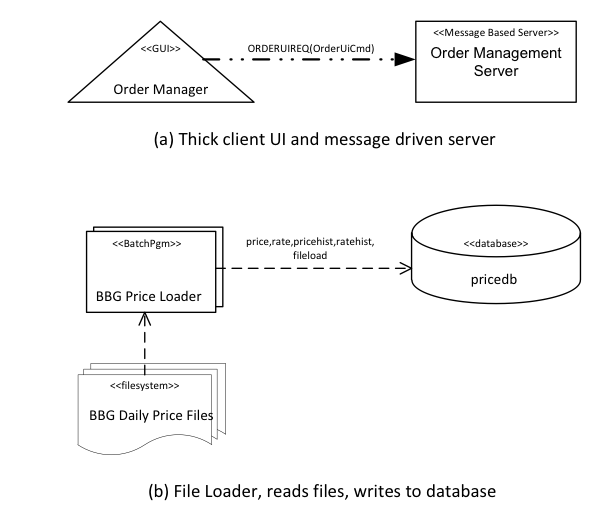
\includegraphics[width=10cm]{Figures/adls-figure1}
\caption{Examples of the ADL Notation Illustrating Preferred Configurations}
\label{figure:adlnotation1}
\end{figure}  

  The notation used to express the examples is explained more fully in the next section, but briefly triangular shapes represent user interfaces, rectangles represent server resident elements (servers, batch programs), files and databases are represented by the fairly conventional "record stack" and "drum" shapes, while connectors are represented by arrows using a variety of line types (the line type in example (a) being messaging, the line type in example (b) being stored data access).

\subsection{The Architecture Description Language}

  Once the universe of required element and connector types was understood, we needed a notation that would allow instances of the style (i.e. the subsystems) to be clearly represented.  As explained earlier, we decided to define a custom notation because the initial discussions with the teams had made it clear that getting people to use a specific tool or invest much effort in learning the notation was going to be very difficult. This was a key reason for creating a very simple notation and "just drawing pictures" rather than trying to apply a general-purpose notation or create machine readable models.

  Given people's general enthusiasm for diagrams over text, we chose to create a graphical notation rather than a more formal textual one. We could have created an equivalent textual notation to provide an alternative concrete syntax, but we didn't need one for this project and as we were not trying to create a reusable ADL we had no reason (or the time) to create alternative notations.

  When defining the graphical detail of the notation, the advice in [27] were particularly useful, in particular the exhortation to avoid construct overload, deficit, redundancy or excess, the suggestion to systematically consider the visual variables of each shape (shape, size, colour, orientation, brightness and texture) and the need for deliberate selection of shapes so that their appearance suggested their meaning, to help achieve semantic transparency.

  We created the graphical notation by selecting a base shape for each major type of element (server, user interface, data store, external entity) and designing a variation of the shape for each subtype of the element.  The diagrams were likely to be printed in black and white, so brightness and colour were used in a very limited way (just being used as an informal diagrammatic annotation, rather than having a predefined meaning).  Each element had to have a name, shown on its symbol and optionally a stereotype (discussed below).  Examples of the notation for some of the more important element types are shown in Figure \ref{figure:adlelementtypes}. 
  
\begin{figure}
\centering
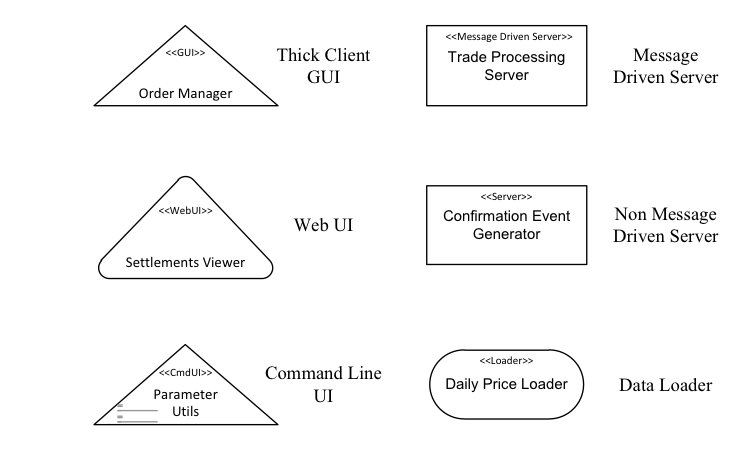
\includegraphics[width=10cm]{Figures/adls-figure2}
\caption{ADL Element Types}
\label{figure:adlelementtypes}
\end{figure}  


  A triangle was used as the base shape for user interfaces and a rectangle for server resident components.  The triangle was chosen as it hinted at the head and shoulders shape of a user and the triangles were then modified slightly for each type of user interface (the thick client having sharp corners, the web user interface having rounded corners as it blurs the distinction between "client" and "server" and the command line utility having a graphical representation of a command line interface added to it).  Similarly, a rectangle is the base shape for server elements (based on long accepted conventions) with a stereotype being used to indicate the type of server and a "lozenge" variant being used to indicate a data loader (hinting at pieces of data being transmitted through it).

  An arrow of some form was used to represent all of the connector types, with the arrowhead usually indicating the direction of data flow.  All connectors were defined to be one way connections, with the exception of data access connectors, which could indicate read and write activity with arrow heads at both ends of the connector if appropriate.  The convention for RPC connectors was defined to be a one-way arrow from the caller to the target.  No attempt was made to represent the various complicated possibilities of dependency and initiation of interaction using the connector symbols.  Each connector had to indicate what was carried over the connection, with message flows being annotated with a message data type, file and database connectors being annotated with table or record names, and RPC and direct invocation connectors being annotated with the name of the service or procedure they were calling.  Examples of the notation for the main connector types are shown in Figure \ref{figure:adlconnectortypes}. 

\begin{figure}
\centering
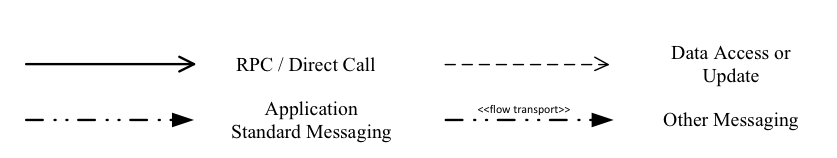
\includegraphics[width=10cm]{Figures/adls-figure3}
\caption{ADL Connector Types}
\label{figure:adlconnectortypes}
\end{figure}  


  The RPC or direct procedure call is shown using a solid arrow, messaging is shown using a line with embedded dots, suggesting messages flowing over it, while data access is shown using a regular chain line, suggesting records being read or written over the connector.

  A general mechanism used on elements and connectors was the stereotype, adopted from UML, where the type of an architectural element is made clear by annotating it with a type name using the 
convention "{\guillemotleft}type{\guillemotright}" on the symbol concerned.  This allowed the casual reader to understand the types of element on the diagram without having to understand the notation and allowed new element types to be easily introduced.

  The semantics of the elements and connectors were generally based on the semantics of the corresponding element and connector implementations in the system: broadcast messaging in the system worked in a particular way, a relational database has well understood behaviour, a web service call is widely understood and a message driven server was a concept that most people understood with little further explanation.  Undoubtedly there were cases where elements on diagrams had surprising behaviour because they did not behave entirely as expected given their type, but on the whole, the resulting documents were good enough to form a useful architecture description.

  In order to ensure that the process produced more than just pictures, we defined a set of required attributes for each type of element and connector.  Part of this task was defining enumerations of expected standard values for many of the attributes, again to standardise and simplify the process of recording the information (such as standard lists of data domains ["trading", "counterparties", "securities", ...], lists of programming languages in use [C++, Java, C\#, Perl] and so on).

  In order to simplify and standardise the subsystem descriptions, a set of wiki page templates and a comprehensive Microsoft Visio stencil were created, along with clear instructions, quick reference material and - most crucially - a fully worked example of the documentation for one subsystem.  This allowed a number of conventions, such as hyperlinking element names to allow navigation through the documents, to be illustrated and encouraged by example.  A hierarchy of empty wiki pages for the required subsystem descriptions was also created so that authors knew where to put their documents and so they could be unambiguously referenced.

  The result of this process was a relatively informal definition of a simple ADL with a graphical notation and set of well-defined conventions for storing the supporting text needed to explain and fully define the subsystem descriptions.  The ADL is tied very strongly to the particular architectural style of this system (its element and connector types) and we deliberately did not attempt to generalise the language, as this very tight link to the system to be described was one of its major strengths for our situation.  In this way, our ADL is rather like the ADLs defined to support specific implementation frameworks like DAOP-ADL [29] which was developed to describe DAOP applications [30] and CBabel [31] which was developed to allow the definition of CR-RIO applications [32].

\section{A Case Study of the Approach in Use}

  The system described in the case study is the Asset Management System (AMS) a financial asset management system used by a fund manager to support making and executing investment decisions for a large-scale investment portfolio.  The example is based on a real subsystem from the case study, modified slightly in order to retain anonymity.

  The primary aim of the system is to allow a fund manager (or fund management team) to manage a portfolio of holdings in financial instruments (primarily equities in this case).  The system must allow them to view the content of their portfolios and to use analytical tools and market data (such as prices, volatilities, projected interest and foreign exchange rates and projected bond yields) to make investment decisions.  The system provides the ability for suggested changes to portfolios to be automatically calculated on demand or from a temporal schedule and also allows direct entry of orders to buy or sell securities to allow for investment strategies that are outside the scope of the system.  Once lists of orders to buy or sell securities are generated, the system allows them to be dispatched to another system for execution and it receives the results of the execution of those orders in return, to allow the current holdings to be updated.

\subsection{Architectural Description}

  The functional structure of the AMS is described using our system-specific ADL 
notation in Figure \ref{figure:amsdiagram}. 

\begin{figure}
\centering
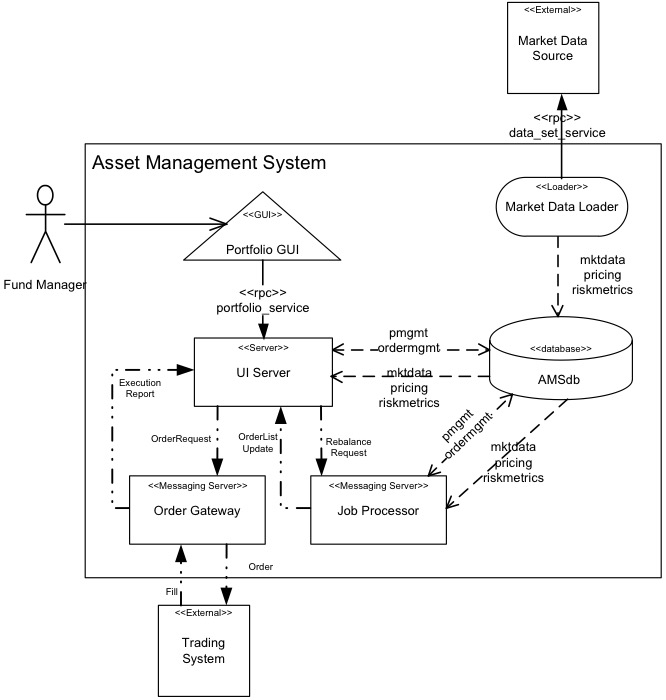
\includegraphics[width=10cm]{Figures/adls-figure4}
\caption{The Asset Management Systems}
\label{figure:amsdiagram}
\end{figure}  

The elements of this architectural structure are described in Table \ref{table:amselements}. 
  
\begin{table}
\caption{Elements of the Asset Management System}
\label{table:amselements}
\footnotesize
\begin{tabular}{l l p{7cm}}
Element Name & Type & Description \\
\hline

Portfolio GUI      & GUI              & The responsibilities of the Graphical User Interface (GUI) are to provide the asset managers using the system with the ability to view and analyse their portfolios, to request (and monitor progress of) long running system operations (such as order generation) and to check, enter, dispatch and monitor orders that go for execution to trading systems.  The GUI provides a human interface and requires an RPC interface to the UI Server to provide it with services and data. \\

UI Server          & Messaging Server & The responsibility of the UI Server is to provide the data access facilities that the UI requires (accessing data from the AMSdb internal database) and to dispatch requests for orders or for long running work (such as analysis processing) to be carried out by other parts of the system.  The UI Server provides an RPC interface to expose its provided services to the GUI and requires an SQL query interface to the system database and a messaging interface to allow it to request and monitor order dispatch and long running work. \\

AMSdb              & Database         & The system database's responsibility is to store the portfolio, analytical, market and (system) operational data that the system requires to operate.  It provides an SQL based DML interface to allow data to be inserted, manipulated or retrieved. \\

Job Processor      & Messaging Server & The responsibilities of the Job Processor are to execute long running processing items ("jobs") such as investment analytics and automated order list generation.  The processor can be configured to run particular jobs on temporal schedules and can also be requested to execute particular jobs on demand.  The processor provides a message based job control and status request interface and requires an SQL query based interface to the database. \\

Market Data Loader & Loader           & The responsibility of the Market Data Loader (MDL) is to retrieve various forms of market data from an internal Market Data Source system and load the data into the database, handling versioning and business date identification as part of the loading process.  The datasets required include securities prices, bond yields, interest rates, FX rates, volatilities, correlations and so on.  The loader requires a data retrieval interface to the MDL system, allowing data sets to be retrieved on demand. \\

Order Gateway      & Messaging Server & The responsibility of the Order Gateway is to accept incoming orders to buy and sell securities (including order parameters such as execution strategies and price limits), to forward these requests to a trading system for execution and then receive the execution reports ("fills") indicating order execution and broadcast these to other interested parts of the system.  The gateway provides a message based order request interface and a broadcast status interface and it requires a message based interface to allow order submission to a trading system.
\end{tabular}
\end{table}

\subsection{Example Scenario - Generate Order List}

  The key functional scenario for this system is to allow a fund manager to generate an order list to "rebalance" a fund based on an analysis that identifies the theoretically optimal holdings for the portfolio and execute that set of buy and sell orders, reflecting the results in the portfolio.  The interactions required to implement this scenario are illustrated in Figure \ref{figure:rebalanceinteractions}. 

\begin{figure}
\centering
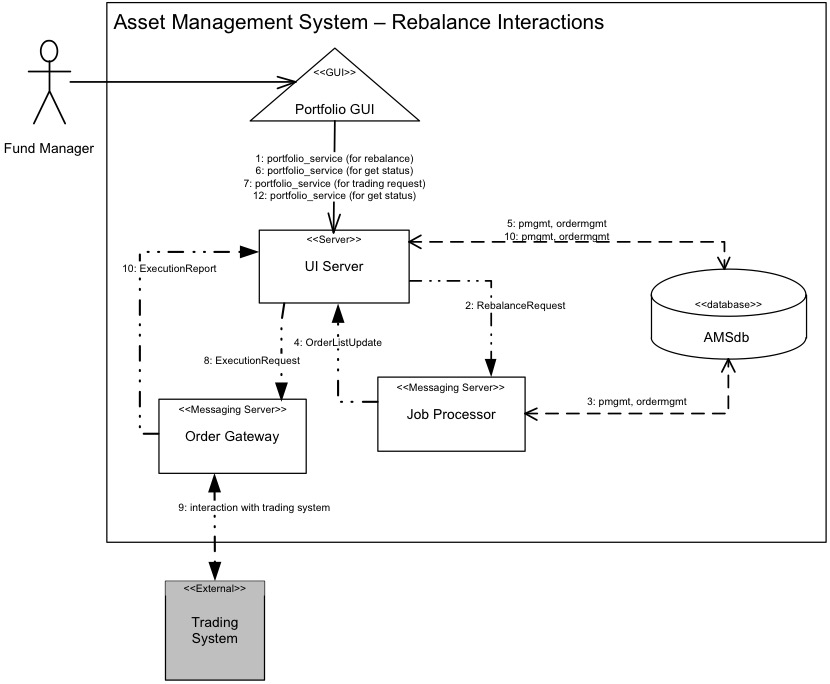
\includegraphics[width=10cm]{Figures/adls-figure5}
\caption{Portfolio Rebalance Scenario Interactions}
\label{figure:rebalanceinteractions}
\end{figure}

The interactions between system elements necessary to implement this scenario are described in Table \ref{table:amsinteractions}. 
  
\begin{table}
\caption{Interactions for the Portfolio Rebalance Scenario}
\label{table:amsinteractions}
\footnotesize
\begin{tabular}{l l l l p{2cm} p{5cm}}
Step & From & To & Type & Connector & Description \\
\hline

1 & GUI & UI Server & RPC & portfolio service & Fund manager selects a portfolio and instructs the system to create an order list for it.  The GUI invokes an RPC indicating that the indicated portfolio should be rebalanced. \\

2 & UI Server & Job Processor & Msg & Rebalance Request & The UI Server sends a request message to indicate that the portfolio should be "rebalanced".  This is routed to the Job Processor. \\

3 & Job Processor & AMSdb & DB & pmgmt and ordermgmt schemas & The Job Processor receives the message and in response initiates a portfolio analysis job to identify the theoretical optimal holdings in the portfolio and generate buy and sell orders to move the portfolio to that state.  Portfolio state read from "pmgmt" and order lists written to "ordermgmt" \\

4 & Job Processor & UI Server & Msg & OrderList Update & The Job Processor sends a status message indicating that new order lists exist, which is routed to the UI Server \\

5 & UI Server & AMSdb & DB & ordermgmt and pmgmt schemas & The UI Server accesses the database to get the new portfolio state and associated order list state \\

6 & GUI & UI Server & RPC & portfolio service & The GUI calls the UI Server for a status update and gets details of the new order list in return \\

7 & GUI & UI Server & RPC & portfolio service & The GUI makes an RPC call to the UI Server to indicate that the order list should be traded \\

8 & UI Server & Order Gateway & Msg & Execution Request & The UI Server creates a message to request the order list to be traded (including the list of orders) which is routed to the Order Gateway \\

9 & Order Gateway & Trading System & - & - & The Order Gateway sends the orders to an external trading system and receives status updates in return as the orders are executed \\

10 & Order Gateway & UI Server & Msg & Execution Report & As the Order Gateway gets execution updates, it creates execution report messages which are routed to the UI Server \\

11 & UI Server & AMSdb & DB & pmgmt and ordermgmt schemas & The UI Server updates the database with the status of the orders and the effect on the portfolio \\

12 & GUI & UI Server & RPC & portfolioservice & The GUI makes RPC calls to the UI Server and gets the updated status of the orders and the changes to the portfolio in its response \\

\end{tabular}
\end{table}

  A full architectural description for a subsystem would also include a lot of operational and implementation oriented information such as links to operational instructions, links to source code control systems and automated build systems and links to test specifications and results.  We do not attempt to reproduce any of that here as the majority of such information was in the form of links to other internal systems and nearly all of the information is context dependent and so not particularly meaningful outside the organisation operating the system.

\section{Experience Gained}

\subsection{Creating the Architecture Description}

  As mentioned earlier, two experienced architects led the project to create the architecture description, which included identifying the underlying architectural style, defining a clear approach, defining the ADL and leading the work to capture the architectural descriptions.  There were approximately 20 development teams who owned significant subsystems that needed to be included in the scope of the project.

  In order to organise the work, the development teams were ranked in order of the criticality of their subsystems in terms of how central they were to key organisational workflows and this acted as an ordered backlog of work for the architects.

  The general approach taken to the task was simple and involved approaching each team and asking for a single person to be nominated as the owner of their documentation.  A conference call was then held with this person and the group manager to explain the project and the approach.  The team was asked to commit time and effort to completing their documents and to commit to a timeline for completing the agreed deliverables (a team often had a number of subsystems that needed to be documented and for planning purposes the creation of a subsystem description was decomposed into some standard subtasks).  In return, the architects leading the effort offered training, practical assistance (such as drawing diagrams) and to review the descriptions produced.

  The interactions with different teams varied greatly, with some teams producing their documentation largely unaided, needing only some review and minor correction, while others were simply incapable or unwilling to produce what was needed and the architects ended up writing most of the documentation for these teams. 

  The reasons for the problems encountered with development teams varied.  In some cases it was simply a lack of interest, often from the development manager who perhaps didn�t see the value of the deliverables.  However in other cases there seemed to be a genuine difficulty in understanding how to represent their subsystem.  In general this seemed to stem from an inability to abstract away from the implementation, resulting in a confusing mix of concrete and totally abstract concepts, which they then struggled to relate to each other.  None of these subsystems were very difficult to represent and in order to make progress the architects often stepped in and simply created the models.

  Another interesting problem was tooling.  Everyone in the organisation had access to the wiki and knew how to use it, so document authors could fill in the tables and text without any difficulty.  However, not everyone had access to Microsoft Visio and even of those that did, some obviously didn't know how to use it.  Again, the solution to this was simply for the architects overseeing the process to create diagrams for some subsystems.  This was a useful lesson and provided further evidence that avoiding UML and more specialised modelling tools had been a good decision.  In this organisation, requiring the use of UML and modelling tools would have been a significant barrier to getting architectural descriptions created.

  Over time, a significant and useful body of subsystem descriptions emerged and this allowed the architects to create a summary level architecture description that showed how the subsystems related to each other.  Some use of scripting to process the wiki subsystem descriptions and drawing tool macros to generate parts of the summary level diagrams allowed some degree of automation, although it was still a fairly manual process.

   The process of capturing the architecture description took about six months, with the architects working on it approximately 60\% of their time and the development teams working on it as their project schedules allowed.

\subsection{The Results of the Project}

  The outputs of the project were as follows.

\begin{itemize}
\item A fairly consistent architecture description for most of the system that provided an accurate and largely complete view of its subsystems, their components and their dependencies.  Each subsystem was described using a standardised approach, which captured the same information for each one and presented it in a consistent manner through the use of the templates provided.  This made the information provided easy to navigate and check for completeness.

\item An informal definition of the architectural style used across most of the system and the typical patterns used when implementing it.

\item A degree of visibility and understanding of the structure, scale and interconnectedness of the system which hadn't been achieved before.  The consistent presentation of system design information in a single location allowed the overall system structure to be more easily understood compared to the previous inconsistent descriptions on scattered wikis and web sites.  This appeared to allow a number of senior technical managers to achieve new insights into the system.

\item An insight into the degree of implementation uniformity between the different subsystems of the application.  While many subsystems were implemented in a very similar way, like any large system (particularly one which has had other applications integrated into it), parts of this application were implemented in ways that didn't follow the normal set of conventions.  While there was already a general awareness that these less standard subsystems existed, the models made it easier for senior technical staff to gain visibility of this and decide whether they wished to direct any changes to the application as a result.

\end{itemize}

  As mentioned earlier, the project did not have particularly clear goals for the architecture description once developed.  A number of people did find it insightful and there seemed to be a general consensus that it was a useful description to have.  However organisational changes then meant that the architects involved moved on to other work, so the project effectively came to an end.  Since then however another group within the firm has adopted the architectural description and continued its use and maintenance (primarily to support production operation of the system, a use which was not foreseen at the outset of the project).

  

\subsection{Evaluating the Usefulness of the ADL}

  Early practical experience led to some rapid refinement of the notation to remove ambiguities that had not been apparent to its creators, and to introduce some missing concepts.  However, after three or four teams had used the approach over a period of about 6 weeks, the ADL itself remained stable for the rest of the project.

  As the project neared completion we started to validate what was being produced with some of the important stakeholders, particularly the senior technical managers in the organisation.  To do this we met with them and demonstrated what was being produced and what the completed architectural description would contain, discussing possible uses of it (such as impact analysis, pre-implementation reviews, incident post-mortems and regulatory enquiries).  We were pleased to find that this stakeholder group reacted positively to what they were shown, with responses ranging from fairly neutral (where the possible usefulness was acknowledged but no specific use of it particularly interested them) to very positive (where they wanted to start using it immediately).  Given this informal but consistently positive sentiment, we felt that our notation and approach had been validated (an outcome which was anything but certain at the start of the project, when the use of a specific notation and a highly prescriptive form for the documentation had been viewed as very risky). 

  A factor that was constant throughout the project was that teams who had the ability to identify clear abstractions for their subsystems also appeared to find the ADL helpful and straightforward to use, as the ADL gave them a clearly defined way to represent their models and they didn't have any difficulty in representing their models using it.  These teams tended to create their models with little or no assistance once they'd asked a few clarifying questions about the purpose of the models and the semantics of the notation.

  In contrast, teams who struggled to identify good abstractions never really grasped how to use the ADL and needed constant assistance, to the point of needing to have parts of their architectural descriptions completely rewritten for them.   What was interesting about this stark contrast in modelling ability was that we could find no obvious factor to explain it in terms of educational background, age, team size, technology preferences, type of subsystem, geographical location or any other relevant factor.  We did observe that even in teams that produced good models, the ability and enthusiasm to do this varied and even for large subsystems we found that it tended to be one or two people in a team who did all of the modelling on behalf of the rest of the team.  We don't know whether there were many other people in those teams who would have done an equally good job, but based on hallway conversations, we suspect not.  Our conclusion was that relatively few people in the general population of software engineers we worked with find modelling straightforward, but we were not sure why this was the case.

  We interpreted this experience as validation of the approach that had been used.  People who could create models and knew what they wanted to represent were able to use the ADL effectively with minimal training, so it was obviously usable by mainstream practitioners.  On the other hand, the approach did not help those people who found it difficult to create a model.  It had been hoped that the straightforward and prescriptive nature of the approach would guide people to create useful models, even if they did not find modelling easy, and it was a disappointment that the approach failed to achieve this.

  Looking back to the success criteria we had set ourselves at the start of the project, we considered whether the architectural description we had created was useful for our three goals to create a catalogue of what was there, to allow impact analysis and to facilitate communication (see Section 4).
  
\begin{itemize}

\item Create a Catalogue of the Current State - the project created the first comprehensive description of the system and so provided a very useful descriptive catalogue of the current state of the architecture.  The weakness of the architectural description as a catalogue was that it was only as comprehensive as the authors of each piece decided to make it.  However, it was possible to cross check it against a number of systems that were known to contain complete lists of the elements in the production system (as they were used for automated tasks relating to deployment).  Sampling about 30 percent of the architectural description and cross checking this against the lists of deployment elements revealed a high degree of completeness, so confidence in its use as a catalogue was high.

\item Allow Impact Analysis - the architectural description quickly proved its worth for impact analysis and helped considerably with the process of understanding the impact of proposed changes.  This was primarily due to the fact that it allowed the interconnectedness of system elements to be quickly assessed, information that hadn't been easy to find before.  An example of this was a small project to migrate the interface to an important internal service from a legacy RPC technology to the currently strategic message based interface.  The service interfaces were designed so that they could be used in parallel and the plan was to offer both and then slowly migrate users of the service to the new version.  The problem with this was the time it was going to take to find all of the users of the service and so the length of time that the parallel interfaces would be needed.  The model was in a late state of development when this project started to think about migration and they were able to use it to discover nearly all of the clients of their service.  So rather than relying on a service provider keeping track of the users of the service, the model provided a structure to allow the users of the service to declare their interest in the services they used, which was a much more effective approach.

\item Communicate - the architectural description was quickly recognised to be a comprehensive knowledge base of the system's design information and so helped inter-team communication (when people in one team could use it to understand another team's subsystem).  An example of the model being used for this sort of collaboration was when a new application, which had been acquired as part of the acquisition of another firm, was being integrated into the existing application as a new subsystem.  The existing models helped the new team see how existing subsystems were integrated with each other and the model that the new team created of their subsystem helped the existing teams to understand what was being added to the system and how it might be used.  The architectural description also acted as a single place where further information could be gathered.  As mentioned earlier, the architects involved in creating the architectural description moved onto other work soon after its initial creation, however it does appear to have continued to be used, to grow and to evolve, suggesting that it did fulfil this role.  Eventually it was adopted by the Production Services team in the firm, due to the value that they got from having up to date descriptions of the structure and dependencies of each application, for support tasks.

\end{itemize}

  Based on this fairly informal assessment, we judged the project to have met the goals we set for ourselves and the architectural description became a useful resource within the organisation, as a centralised and standardised source of design information for the system.

\section{Lessons Learned From The Project}

  At the start of the project, no one involved in it had much experience in using ADLs in an industrial context.  The experience the architects had between them was limited to some simple use of ADLs in an academic context and some significant experience of using UML for architectural modelling in large industrial projects.  Therefore, we had relatively few preconceptions as to how successful the project would be and on the whole we were pleased with its results.

  The main lessons that were learned during the course of the project were:
  
\begin{itemize}

\item A specialised ADL can have benefits over a general modelling language like UML and even a simple ADL can be used to create useful results.

\item The more specialised an ADL is, and so the closer it matches the implementation style of the system being modelled, the easier people seem to find it to use.  While at first glance this sounds like an obvious point, it is contrary to the conventional industrial approach of using a general modelling language like UML or SysML and also contrasts with the domain independent nature of most academically developed ADLs.

\item Carefully designing the detail of the graphical notation pays off.  Using shapes that hint at their meaning and using a range of graphical dimensions to differentiate shapes helps people to remember them, even if they don't guess the link between the shape and the concept themselves.  Again, this is not reflected in mainstream notations like UML or most existing ADLs, where little effort is made to identify meaningful symbols for concepts.

\item Consistency in the notation is very important and having a base shape for a general concept with refinements to it for different sub-concepts appears to help people considerably when interpreting the diagrams.

\item Providing high quality support materials including an example-based description of the approach and notation, a number of realistic completed examples and a set of templates for new documents is very important.  We found repeatedly that people are much better at "filling in the gaps" rather than following a set of instructions and creating something from scratch.

\item Utilising familiar tools helps with the acceptance of the approach.  In this particular organisation, there were no complaints or difficulties with the use of a wiki for the text and tables information, whereas a very widely used commercial drawing tool (Visio) caused problems, even with a carefully tailored template, because it was not widely used in the organisation already.

\end{itemize}

  These lessons aren't all that surprising but the importance of what seemed to be quite minor things (such as worked examples and quick reference cards) is important and is useful to bear in mind for the future.  The importance of matching the ADL to the specific domain being modelled is also a lesson that is not reflected in most modelling languages today, which tend towards the general rather than the specific.  

  Given the relative success of this project, it is natural to ask how generally applicable its results are and how repeatable it is likely to be.  Given what we learned during the project, particularly the fact that the specialised nature of the notation was a key factor in its success, we feel that these lessons may well have general applicability, but only in the broad sense.  People like to be guided and they like familiar tools and techniques.  However the specific tools or techniques that work will be specific to each environment and people in different environments will have different levels of enthusiasm for learning new approaches.  However, when trying to get a significant amount of work done by people who are agnostic to the approach, familiarity and accessibility appear to help greatly with acceptance.

  Based on our experience, the specific suggestions that we would make for future modelling languages are as follows:

\begin{itemize}
\item Create a language that is specific to a domain (e.g. real-time control systems or enterprise information systems) and ensure that it contains the type of modelling elements needed in that domain.  Modelling languages also need to be easily extensible by their users, rather than modelling language experts, to allow missing element types to be added.  Of course specialising a language limits its possible user community, but conversely that user community is more likely to find a language that matches their problems useful and so are more likely to use it.

\item Spend time creating a rich visual notation that communicates as much as possible using the shape, line, fill and other visual aspects of the notation.  This makes diagrams much easier for people to understand.

\item Keep modelling languages as simple as possible so that people can start using them quickly without a great deal of training.  We have observed that modelling language constructs with complex or obscure semantics are rarely used correctly, if they are used at all.

\item Consider how people will use the language and what they will need in terms of tools and facilities for structuring and managing large models.  Again simple tools (and ideally extensions to tools that people are already likely to be familiar with) are much more likely to be successful than tools that require a lot of training and experience to use.

\item As well as the language and tools, develop the materials that people will need in order to successfully adopt the language for practical use.  This includes task oriented training material, quick reference guides and plenty of samples which show the value of the language in use and provide people will examples of how to use it well (which they will almost certainly copy).
\end{itemize}

  It is worth noting that our experiences from this work and our resulting suggestions are similar to the conclusions of a major academic survey of practitioner requirements for ADLs [33], which suggests that these lessons and requirements reflect the needs of a significant number of industrial software architects.

  Beyond the experience we have gained in applying architectural description techniques to a large scale problem, the particular notation and approach used in this paper may be of use to others, but as explained earlier in the paper, this wasn't a goal of the project. While some of the aspects of the notation invented will be generally familiar (e.g. servers that are driven by messaging) the overall set of element types is specific to one environment and may well not be directly useful elsewhere.  Certainly we did not set out to contribute yet another general purpose ADL to the world and so reuse of the notation was not considered during its development.  We report this project in order to describe a successful application of the concepts of architectural description notations, to record the factors that we believe made the project successful and to capture the lessons learned and conclusions drawn from the experience.

\section{Summary And Conclusions}

  An organisation in the financial services industry wanted to create an architecture description for a large existing enterprise system.  In order to achieve this within acceptable cultural and time constraints a simple, custom architecture description language was defined in order to make the process of capturing the architecture description as simple and prescriptive as possible.

  While it was not clear at the outset whether this approach would be successful, the ADL actually proved to be a helpful and effective tool for capturing this specific architecture description in an entirely industrial context.  A large architecture description was created, something that the organisation had not achieved before, and this allowed new perspectives on the system to be gained.

  What the approach did not achieve was helping those who found modelling difficult to create effective models.  People who found abstraction difficult seemed to find it just as difficult when using this very specific approach as when using a general-purpose notation, which was a surprise and a disappointment.

  Having said that, the factor that appeared to make the approach generally successful was focusing on describing the specific structures in the system of interest, rather than trying to create a general-purpose approach, which would be effective for other uses too.  Other factors which contributed to the success of the approach were its simplicity (which traded sophistication for accessibility), a carefully designed, consistent graphical notation, the availability of a large amount of tutorial and reference material to guide document authors, and the use of very familiar tools, which users of the notation were already familiar with.

\section{References}

[1]	D. Di Ruscio, I. Malavolta, H. Muccini, P. Pelliccione, and A. Pierantonio, "ByADL: an MDE framework for building extensible architecture description languages," in Proceedings of the 4th European Conference on Software Architecture, Copenhagen, Denmark, 2010, pp. 527-531.

[2]	P. Cuenot, P. Frey, R. Johansson, H. Lonn, Y. Papadopoulos, M.-O. Reiser, et al., "The EAST-ADL architecture description language for automotive embedded software," in Proceedings of the 2007 International Dagstuhl conference on Model-based engineering of embedded real-time systems, Dagstuhl Castle, Germany, 2010, pp. 297-307.

[3]	F. Oquendo, "�-ADL: an Architecture Description Language based on the higher-order typed �-calculus for specifying dynamic and mobile software architectures," ACM SIGSOFT Software Engineering Notes, vol. 29, pp. 1-14, 2004.

[4]	R. Bashroush, I. Spence, P. Kilpatrick, and T. Brown, "Towards More Flexible Architecture Description Languages for Industrial Applications," in EWSA 2006. vol. 4344, V. Gruhn and F. Oquendo, Eds., ed Nantes, France: Springer-Verlag, 2006, pp. 212-219.

[5]	E. Woods and R. Hilliard, "Architecture Description Languages in Practice," in the 5th Working IEEE/IFIP Conference on Software Architecture (WICSA 2005), Pittsburgh, PA, 2005, pp. 243 - 246.

[6]	R. van Ommering, F. van der Linden, J. Kramer, and J. Magee, "The Koala component model for consumer electronics software," IEEE Computer, vol. 33, pp. 78-85, 2000.

[7]	R. Allen, S. Vestal, D. Cornhill, and B. Lewis, "Using an architecture description language for quantitative analysis of real-time systems," in Proceedings of the 3rd international workshop on Software and performance, Rome, Italy, 2002, pp. 203-210.

[8]	P. Feiler, B. Lewis, and S. Vestal, "Improving Predictability in Embedded Real-Time Systems," Software Engineering Institute, Carnegie Mellon University, Pittsburgh, Pennsylvania2000.

[9]	H. Lonn, T. Saxena, M. Torngren, and M. Nolin, "Far east: Modeling an automotive software architecture using the east adl," 2004.

[10]	N. Medvidovic and R. N. Taylor, "A classification and comparison framework for software architecture description languages," IEEE Transactions on Software Engineering, vol. 26, pp. 70-93, 2000.

[11]	P. C. Clements, "A Survey of Architecture Description Languages," in Proceedings of the 8th International Workshop on Software Specification and Design, 1996, p. 16.

[12]	"Standard AS5506/1: SAE Architecture Analysis and Design Language (AADL)," ed: SAE International, 2006.

[13]	D. Garlan, R. T. Monroe, and D. Wile, "Acme: architectural description of component-based systems," in Foundations of component-based systems, T. L. Gary and S. Murali, Eds., ed: Cambridge University Press, 2000, pp. 47-67.

[14]	K. Dunsire, T. O'Neill, M. Denford, and J. Leaney, "The ABACUS Architectural Approach to Computer-Based System and Enterprise Evolution," in Proceedings of the 12th IEEE International Conference and Workshops on Engineering of Computer-Based Systems, 2005, pp. 62-69.

[15]	R. Allen, "A Formal Approach to Software Architecture," PhD thesis, Computer Science, CMU, Pittsburgh, 1997.

[16]	M. Shaw, R. DeLine, and G. Zelesnik, "Abstractions and implementations for architectural connections," in Proceedings of the 3rd International Conference on Configurable Distributed Systems, Annapolis, Maryland, 1996, pp. 2-10.

[17]	R. Allen and D. Garlan, "The Wright Architectural Specification Language," Carnegie Mellon University, Software Engineering Institute, Pittsburgh, PA1996.

[18]	D. Batory and B. J. Geraci, "Composition Validation and Subjectivity in GenVoca Generators," IEEE Transactions on Software Engineering, vol. 23, pp. 67-82, 1997.

[19]	D. C. Luckham, J. J. Kenney, L. M. Augustin, J. Vera, D. Bryan, and W. Mann, "Specification and analysis of system architecture using Rapide," IEEE Transactions on Software Engineering, vol. 21, pp. 336-354, 1995.

[20]	M. Moriconi and R. A. Riemenschneider, "Introduction to SADL 1.0: A Language for Specifying Software Architecture Hierarchies," SRI International,1997.

[21]	R. Khare, M. Guntersdorfer, P. Oreizy, N. Medvidovic, and R. N. Taylor, "xADL: enabling architecture-centric tool integration with XML," in Proceedings of the 34th Annual Hawaii International Conference on System Sciences, 2001, p. 9 pp.

[22]	R. Bashroush, T. J. Brown, I. Spence, and P. Kilpatrick, "ADLARS: An Architecture Description Language for Software Product Lines," in Proceedings of the 29th NASA/IEEE Software Engineering Workshop (SEW'29), Greenbelt, MD, 2005, pp. 163-173.

[23]	R. Bashroush, I. Spence, P. Kilpatrick, T. Brown, W. Gilani, and M. Fritzsche, "ALI: An Extensible Architecture Description Language for Industrial Applications," in Proceedings of the 15th IEEE International Conference on Engineering of Computer-Based Systems (ECBS), Belfast, UK, 2008, pp. 297-304.

[24]	R. Bashroush and I. Spence, "An Extensible ADL for Service-Oriented Architectures," in Information Systems Development - Towards a Service-Provision Society, G. A. Papadopoulos, W. Wojtkowski, W. G. Wojtkowski, S. Wrycza, and J. Zupancic, Eds., ed New York: Springer, 2009, pp. 227-237.

[25]	M. M. Lankhorst, H. A. Proper, and H. Jonkers, "The Architecture of the ArchiMate Language," in Proceedings of the 10th International Workshop on Enterprise, Business-Process and Information Systems Modeling (BPMDS 2009) held at CAiSE, Amsterdam, Netherlands, 2009, pp. 367-380.

[26]	K. Smolander, K. Lyytinen, V.-P. Tahvanainen, and P. Marttiin, "MetaEdit: a flexible graphical environment for methodology modelling," in Proceedings of the 3rd International Conference on Advanced Information Systems Engineering, Trondheim, Norway, 1991, pp. 168-193.

[27]	D. Moody, "The "Physics" of Notations: Toward a Scientific Basis for Constructing Visual Notations in Software Engineering," IEEE Transactions on Software Engineering, vol. 35, pp. 756-779, 2009.

[28]	M. Shaw and D. Garlan, Software architecture: perspectives on an emerging discipline vol. 1: Prentice Hall Englewood Cliffs, 1996.

[29]	M. Pinto, L. Fuentes, and J.-M. Troya, "DAOP-ADL : An Architecture Description Language for Dynamic Component and Aspect-Based Development," in 2nd international conference on Generative programming and component engineering (GPCE '03), Erfurt, Germany, 2003, pp. 118-137.

[30]	M. Pinto, L. Fuentes, and J. M. Troya, "Towards an aspect-oriented framework in the design of collaborative virtual environments," in Distributed Computing Systems, 2001. FTDCS 2001. Proceedings. The Eighth IEEE Workshop on Future Trends of, 2001, pp. 9-15.

[31]	C. Braga and A. Sztajnberg, "Towards a Rewriting Semantics for a Software Architecture Description Language," Electronic Notes in Theoretical Computer Science, vol. 95, pp. 149-168, 2004.

[32]	O. Loques and A. Sztajnberg, "Customizing component-based architectures by contract," in Component Deployment, ed: Springer, 2004, pp. 18-34.

[33]	I. Malavolta, P. Lago, H. Muccini, P. Pelliccione, and A. Tang, "What industry needs from architectural languages: A survey," Software Engineering, IEEE Transactions on, vol. 39, pp. 869-891, 2013.

  % Ch3 - ADLs & Case Study

\chapter{Prioritising Architectural Effort}

\section{Introduction}

In our practice in the field of software architecture, we have noticed and experienced how complex it is for software architects to prioritise their work.  The software architect's responsibilities are broad and in principle they can be involved in almost any technical aspect of a project from requirements to operational concerns.  In practice, this makes it difficult for an architecture practitioner to prioritise effort to achieve quality properties like energy consumption, which acquiring stakeholders and end-users rarely prioritise explicitly due their lack of immediate visibility.  Other important quality properties that suffer from similar prioritisation problems include security \cite{cisco2016-uksecprioritisation}, performance and availability \cite{ozkaya2008-qualityproperties}. 

However, we also observe that successful experienced software architects appear to be good at focusing their effort effectively, and do manage to create systems which are performant, secure, highly available and, in the future, no doubt energy efficient too. However not all architects are good at this and, anecdotally, we observe that inexperienced architects often find prioritisation of their focus very difficult.  This situation led us to wonder how the experienced architects achieve this balance.  They may use generic time management techniques (like \cite{allen2015-gettingthingsdone}) but we were interested in whether there are common role-specific heuristics which could be taught to new architects.

We decided to investigate this via a questionnaire-based study of a group of experienced architects.  We discovered that there are common heuristics which experienced architects use to prioritise their work and we created a model to capture them.  We then validated the model via an online questionnaire with a much wider group of practitioners and refined the model based on their input.

In this chapter we explain the approach we took and present both the initial model that we created from the results of the interview process and the final, refined, model that we created after the validation process.  The contribution of the work is not specifically the heuristics in the model, indeed most of them are quite familiar to experienced practitioners, but rather the organisation of the heuristics and the validation that they are used by experienced practitioners to guide their work.  We believe that this makes the model a useful reminder for experienced practitioners and an effective teaching aid for new architects who are learning how to perform the role.

\section{Related Work}

When we started investigating this topic, we were primarily interested in how practitioners really worked; However, we also performed a literature search to find related work from the research community.
We did not find any studies investigating the specific topic we were interested in, but an entire architectural method which is directly relevant to helping architects focus their attention is Risk and Cost-Driven Architecture (RCDA) \cite{poort2012-rcda}.  This method transforms the architect's approach from defining finished architectural structures at the start of a project, to working throughout the project to provide a stream of decisions, using the risk and cost of open decisions to prioritise the architect's work.  We were also interested in finding some very specific advice from a very experienced architect and researcher \cite{kruchten2008-architectsdo} that architects should spend 50\% of their time on architecting, 25\% on inbound communication and 25\% on outbound communication.  However, this is anecdotal advice based on personal experience, rather than the sort of survey-based study that we wished to run.

In the research domain, we found a research community interested in prioritisation of requirements \cite{berander2005-reqpriorization, hermann2008-reqprioritization} and a literature review summarising the research in this area in 2014 \cite{Achimugu2014-reqprio-litreview}.  Prioritising requirements is clearly related to how an architect should focus their attention, but it is only one of a range of possible factors that they could use, so this area of research did not appear to be very relevant to our investigation.

Finally, there is a large amount of mainstream business and self-help literature on time management (such as the well-known \cite{allen2015-gettingthingsdone} and \cite{koch1998-8020principle}); However, we were interested in providing more tailored and prescriptive advice to software architects specifically rather than this sort of more general advice.

\section{Research Method}

When planning this research, we selected a qualitative research approach because we needed to explore the "lived-experiences" of expert practitioners by asking them questions to encourage reflection and insight \cite{lapan2012-qualitativeresearch} rather than assessing performance or alignment with specific practices via quantitative means.

The process was organised into four distinct stages.

\begin{description}
	\item [Stage 1] gathering primary data using semi-structured interviews with practitioners.
	\item [Stage 2] analysis of the primary data and creation of a preliminary model.
	\item [Stage 3] validation of the preliminary model via a structured online questionnaire, completed by practitioners in relevant architecture roles (primarily software, solution and enterprise architects).
	\item [Stage 4] analysis of the validation data and refinement of the preliminary model into a final, validated model.
\end{description}

We chose to gather our primary data using semi-structured interviews, where we provided the interviewees with a written introduction to the question we wanted to answer and then some specific questions to start their thought processes. 

The analysis of the primary data was performed using a simple application of Grounded Theory as it is a suitable method for theory building, to understand the relationships between abstract concepts \cite{charmaz2006-groundedtheory}, which described our situation and needs very closely.  We performed initial coding on the primary data and then refined this with a focused coding exercise.  As suggested in \cite{lapan2012-qualitativeresearch}, the process of collection and analysis was a parallel, iterative process, rather than a linear one with fixed phases.  

This exercise produced a set of themes that classify the heuristics that the architects use, as well as the heuristics themselves.  A heuristic had to be mentioned by at least three of the participants (which represented a third of them) for us to consider it significant enough to be included in the model.  We combined the themes and heuristics to form a simple model (the "preliminary model") of how experienced architects go about prioritising their effort. 

Once we had the preliminary model available, we published it at a research conference \cite{woods2017-archpriorisation} and via a LinkedIn post (https://www.linkedin.com/pulse/focusing-software-architects-attention-eoin-woods) and created an online questionnaire aimed at architecture practitioners to allow them to evaluate and comment on the usefulness of the model.  We publicised the survey via LinkedIn, Twitter and via direct email to our network of architecture practitioners.

We received 84 responses to the survey, containing answers to our closed-ended questions to evaluate the usefulness of the model and also received answers to open-ended questions in 50 of the responses.  We used the closed-ended questions to evaluate the usefulness of the model and analysed the open-ended responses to identify themes which needed to be addressed by the model.

The model was validated strongly across respondents from different locations, with different amounts of experience and from different architectural specialisations. Additionally, a small number of themes emerged from the answers to the open-ended questions.  These themes for improving the model were used to revise and extend it slightly, creating an improved final version that reflected the input from the respondents.

A description of the four stages of the research method is presented below, along with the final version of the architectural effort prioritisation model.

\section{Stage 1 - The Initial Study}

Our primary data gathering was performed using a semi-structured, face-to-face survey of 8 experienced software architecture practitioners working across 4 countries.

We found the participants by approaching suitable individuals from our professional networks.  We were looking for practitioners who had a minimum of 10 years' professional experience and who worked as architects in the information systems domain (rather than architects from \textendash for example \textendash embedded systems).  

We focused on the information systems domain because we know from experience that working practices differ between professional domains like information systems and embedded systems.  Hence, we thought it was more likely that we could create a useful model if we limited ourselves to one broad domain, at least initially. 

We deliberately selected candidates that we knew differed from each other in organisation, specialisation and geography to get a reasonably diverse population and avoid obvious sample bias (we discuss the threat of sample bias further in Section \ref{sec:threats}).

Some characteristics of the participants in the study are summarised in the graphs in Figure \ref{figure:participants}.  As can be seen, they represent a range of experience, role type and country.

%%
%% See this page for the magic:
%% https://tex.stackexchange.com/questions/64858/how-to-create-subfloat-figures-two-in-first-row-and-one-below
%%
\begin{figure}
   \begin{subfigure}{.5\linewidth}
      \centering
      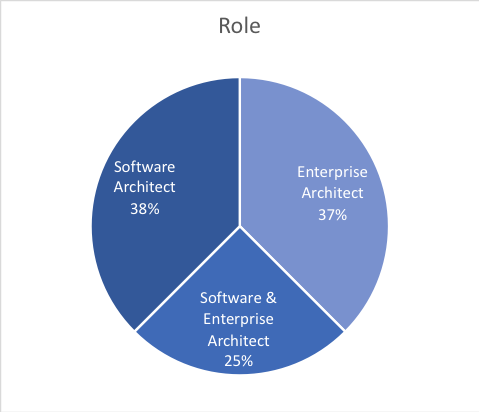
\includegraphics[scale=0.75, trim=5 5 5 5,clip]{Figures/prioritisation-roles}
   \end{subfigure}
   \begin{subfigure}{.5\linewidth}
      \centering
      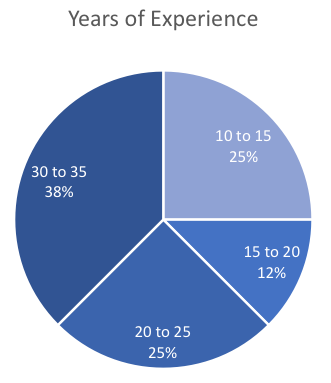
\includegraphics[scale=0.75, trim=5 5 5 5,clip]{Figures/prioritisation-yearsexp}
   \end{subfigure}
   \begin{subfigure}{\linewidth}
      \centering
      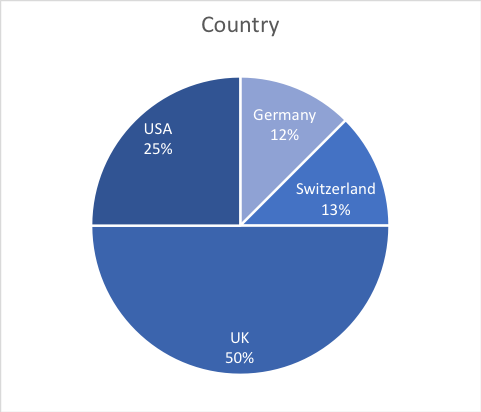
\includegraphics[scale=0.75, trim=5 5 5 5,clip]{Figures/prioritisation-countries}
   \end{subfigure}

   \caption{Study Participants (8 in total)}
   \label{figure:participants}
\end{figure}  

All of our initial practitioner set had over 10 years of post-graduate experience and some had over 30 years of experience, so ensuring that they all had a significant amount of professional practice upon which to base their answers.

We deliberately selected software and enterprise architects because this is who the model was primarily aimed at serving.

We approached individuals in a number of countries to try to minimise the risk that we would reflect practice only in one country, although we did not manage to gain representation from beyond North America and Europe.

We used a semi-structured interview format with a written introduction to the question which each interviewee read before being asked a standard set of open-ended questions which explored how they went about prioritisation of architecture work and any specific factors that they used to guide them.  

The question we asked was "how can the architect concentrate their attention so that they are most effective?" The more specific questions used to stimulate the thought process were: 

\begin{itemize}
	\item How do you go about this in your work? 
	\item What factors do you consider when prioritising your attention? 
	\item Do you consider what to focus on?   Or what not to focus on? 
	\item For example, how do you prioritise architectural governance compared to other aspects of the project?
\end{itemize}

The interviewer asked additional questions to understand the answers fully or to encourage the interviewee to add more detail or fill in ambiguous aspects of the answer.

The process of initial coding of the primary data resulted in 25 items, which could be associated with at least one of the interviews.  A further focused coding process revealed that there were 9 underlying heuristics which appeared to be significant to the participants in the study. Then, a further analysis iteration lead to the identification of three categories of prioritisation heuristic which we use to structure our model.

\section{Stage 2 - Preliminary Model for Prioritising \\Architectural Effort}
\subsection{The Preliminary Model}

Our preliminary heuristic model for focusing architectural effort is shown in Figure \ref{figure:prelmodel}.
 
The three categories of heuristic that the study revealed were firstly, the need to focus on stakeholder needs, secondly, the importance of considering risks when deciding on where to focus effort, and finally the importance of spending time to achieve effective delegation of responsibilities.  These categories form the structure of our model and remind the architect of the general ways in which they should prioritise their efforts. The categories and heuristics are explained in more detail in section \ref{sec:prelim-model-content}.

\begin{figure}
\centering

\includegraphics[width=\textwidth]{Figures/prioritisation-prelim-model}
\caption{Preliminary Model for Focusing Architectural Attention}
\label{figure:prelmodel}
\end{figure}  

It is important to understand the nature of this model and how it should be used.  It is not a prescriptive process for architects to follow or a process for developing an architecture.  This model is an aide memoir to organise and present a set of heuristics that experienced architecture practitioners appear to find useful when prioritising their work.  While we believe this to be a useful model to teach trainee architects, and a useful reminder for experienced architects, it is necessary to apply the model in a context-sensitive manner, within whatever method that the architect is using to develop software architectures.

\subsection{Content of the Preliminary Model}
\label{sec:prelim-model-content}

\subsubsection{Understand the Stakeholder Needs and Priorities}

The first theme which emerged strongly in our study was focusing on the needs and priorities of the stakeholders involved in the situation.  The principle that architecture work involves working closely with stakeholders is widely agreed \cite{rozanski2011-ssa2e, bass2012-sainp} and this theme reinforces that. Architects need to focus significant effort to make sure that stakeholder needs and priorities are understood to maximise focus on the critical success factors for a project and maximise the chances of its timely completion.  Based on the study, three specific heuristics to achieve this were identified:

\begin{itemize}
	\item \emph{Consider the whole stakeholder community}. Spend time understanding the different groups in the stakeholder community and avoid the mistake of just considering obvious stakeholder groups like end-users, acquirers and the development team.  As the architecture methods referenced above note, ignoring important stakeholders (like operational staff or auditors) can prevent the project meeting its goals and cause significant problems on the path to production operation.
	\item \emph{Ensure that the needs of the delivery team are understood and met}.  Spend sufficient time to ensure that the delivery team can be effective.  What is the team good at?  What does it know?  What does it not know?  What skill and knowledge gaps does it have?  These areas need attention early in the project so that architecture work avoids risks caused by the capabilities of the team and that time is taken to support and develop the team to address significant weaknesses.
	\item \emph{Understand the perspective and perceptions of the acquirers of the system}.  Acquirers are a key stakeholder group who judge its success and usually have strategic and budgetary control, so can halt the project before delivery if they are unhappy.  Specifically addressing this group's needs, perceptions and concerns emerged as an important factor for some of the experienced architects in our study.  Acquirers are often distant from the day-to-day reality of a project and need clear communication to understand their concerns and ensure that they have a realistic view of the project.
\end{itemize}

\subsubsection{Prioritise Effort According to Risks}

During a project, an effective approach to prioritising architectural attention is to use a risk-driven approach to identify the most important tasks.  If the significant risks are understood and mitigated, then enough architecture work has probably been completed.  If significant risks are open, then more architecture work is needed. The specific heuristics to consider for risk assessment are:

\begin{itemize}
	\item \emph{Consider external dependencies}.  Understand your external dependencies because you have little control over them and they need architectural attention early in the project and whenever things change.
	\item \emph{Look for novel aspects of domain, problem and solution}.  Another useful heuristic, from the experience of our study participants, is to focus on novelty in your project.  What is unfamiliar?  What problems have you not solved before?  Which technology is unproven?  The answers to these questions highlight risks and the participants in our study used them to direct their effort to the most important risks to address.
	\item \emph{Identify the high impact decisions}.  Prioritise architecture work that will help to mitigate risks where many people would be affected by a problem (e.g. problems with the development environment or problems that will prevent effective operation) or where the risk could endanger the programme (e.g. missing regulatory constraints).
	\item \emph{Analyse your local situation for risks}.  Consider the local factors unique to your situation, which you will be aware of due to the knowledge you have of the domain, problem and solution.  It is impossible to give more specific guidance on this heuristic as every situation is different, but the participants in our study noted the importance of "situational awareness" \cite{wikipedia-sitawareness} that allows the architect to find and address the risks specific to the local environment (perhaps due to organisational factors, specific technical challenges, domain complexities or business constraints).
\end{itemize}

\subsubsection{Delegate as Much as Possible}

Delegation was an unexpected theme that emerged from our study. The architects who mentioned this theme viewed themselves as a potential bottleneck in a project and delegation and empowerment of others was a way to minimise this.  Delegation was also seen as a way of freeing the architect to focus on the aspects of the project that they had to focus on rather than all the other aspects that they could possibly get involved in.

The general message of this theme is to delegate as much architecture work as possible to the person or group best suited to perform it, to prevent individuals becoming project bottlenecks, allow architects to spend more time on risk identification and mitigation, and to spread architectural knowledge through the organisation.  The heuristics that were identified to help achieve this are:

\begin{itemize}
	\item \emph{Empower the development teams}. To allow delegation and work sharing, architects need to empower (and trust) the teams they work with.  This allows governance to become a shared responsibility and architecture to be viewed as an activity rather than something that is only performed by one person or a small group.  This causes architectural knowledge, effort and accountability to be spread across the organisation, creates shared ownership, reduces the load on any one individual and prevents reliance on a single individual from delaying progress.
	\item \emph{Create groups to take architectural responsibilities}.  A related heuristic is to formalise delegation somewhat and create groups of people to be accountable for specific aspects of architectural work.  For example, in a large development programme, an architecture review board can be created to review and approve significant architectural decisions.  Such a group can involve a wide range of expertise from across the programme and beyond, so freeing a lead architect from much of the effort involved in gathering and understanding the details of key decisions, while maintaining effective oversight to allow risks to be controlled and technical coherence maintained.  Similarly, a specific group of individuals could be responsible for resilience and disaster recovery for a large programme, allowing them to specialise and focus on this complex area, and allowing a lead architect to confidently delegate to them, knowing that they will have the focus and expertise to address this aspect of the architecture.
\end{itemize}

\section{Stage 3 - Validating the Preliminary Model}

\subsection{The Questionnaire}

Once we had a preliminary model, we wanted to validate its usefulness with a much larger group of experienced practitioners.  This was conducted using a structured online questionnaire.  The questionnaire asked the respondents to read the model and then comment on its credibility and usefulness.  We asked both closed questions, that asked respondents to rate the model on 5 point scales, and open-ended questions that allowed the respondents to consider whether there were aspects of focusing attention that we had missed and also to collect general comments on the model.  Finally, we asked some closed classification questions to allow us to understand who had completed the survey, while preserving their anonymity if desired.

We asked three closed-ended questions to find out whether the respondent thought that the model was credible and useful.  These questions and the possible responses were:

\begin{description}
	\item [Q1] "Is this model similar to how you focus architectural attention in your work already?" (Not at all similar / Not Very Similar / Somewhat Similar / Quite Similar / Very Similar)
	\item [Q2] "Would you find this model helpful in guiding architectural attention for maximum benefit?" (Definitely Not / Probably Not / Possibly / Probably Yes / Definitely Yes)
	\item [Q3] "Are the areas of risk mentioned in the "Prioritise time according to risks" activity valuable?" (Definitely Not / Probably Not / Somewhat / Probably Yes / Definitely Yes)
\end{description}

The open-ended questions that we asked were:

\begin{description}
	\item [Q4] "Are there other general areas of risk that should be added to "Prioritise time according to risks" that would be applicable to most (information) systems and environments? If so please list and briefly explain them."
	\item [Q5] "Are there any significant factors missing from the model which you use to focus your architectural work?"
	\item [Q6] "Do you have any other comments on the  model or the survey"
\end{description}

The closed-ended questions we asked to allow us to classify the respondents and their possible answers were:

\begin{description}
	\item [Q7] "What environment do you work in?"
	\begin{itemize}
		\item Industry (developing systems, consultancy and related work)
		\item Industrial Research (working in a research environment for an industrial employer) 
		\item Academic (teaching or researching in university or similar environments)
		\item Other (please specify)
	\end{itemize}
	\item [Q8] How many years of post-graduation experience do you have?
	\begin{itemize}
		\item 1-5 years
		\item 5-10 years
		\item 10-15 years
		\item 15-20 years
		\item More than 20 years
    \end{itemize}
	\item [Q9] What is your main job role?
	\begin{itemize}
		\item Software Architect
		\item Enterprise Architect
		\item Software Designer
		\item Researcher
		\item Other (please specify)
    \end{itemize}
	\item [Q10] Where in the world are you based?
	\begin{itemize}
		\item North America
		\item South America 
		\item Europe (including UK) 
		\item Middle-East and Africa 
		\item Asia-Pacific
		\item Other (please specify)
	\end{itemize}
\end{description}

We also invited them to leave an email address if they wanted to be informed of the outcome of the study and provided a free text box for any final comments or questions.  We did not view the email address and the final text box as survey data for the purposes of analysis.

Having trialled the questionnaire ourselves and with two other individuals, we expected most respondents to take 10 – 15 minutes to complete it.

\subsection{The Respondents}

To use the questionnaire to validate the model, we needed to find a suitable set of architects who could read it and complete the survey for us.  We found our respondents via two main activities.  
Firstly, we wrote a LinkedIn post (https://www.linkedin.com/pulse/focusing-software-architects-attention-eoin-woods/) which provided an outline of the model, explained that we wanted to validate it and who we wanted to participate, and provided a link to the survey.  This was posted from my account and so tended to appear in the LinkedIn news feed of practitioners, as my LinkedIn network contains many more practitioners than researchers.  The post was further publicised via Twitter and Facebook to reach a larger audience.  This step was moderately successful, with the post being viewed about 700 times and about 25 people completing the survey successfully.

To gain more responses to the survey, the second activity was a targeted email sent to individuals that we knew personally and who we knew were practicing software related architects (including software, solution and enterprise architects).  This second activity resulted in about 60 more responses to the survey.

In total, we received 84 completed surveys.

The job roles of the respondents are summarized in Figure \ref{figure:resproles}.  About a third of the respondents identified themselves as software architects, about a quarter as enterprise architects, about 12\% as software designers, 10\% as solution architects, and 5\% as technical architects.  Four respondents did not complete this answer and four had other job titles (a risk assessor, a technical manager and systems engineer, a project manager and a strategy consultant).

\begin{figure}
\centering
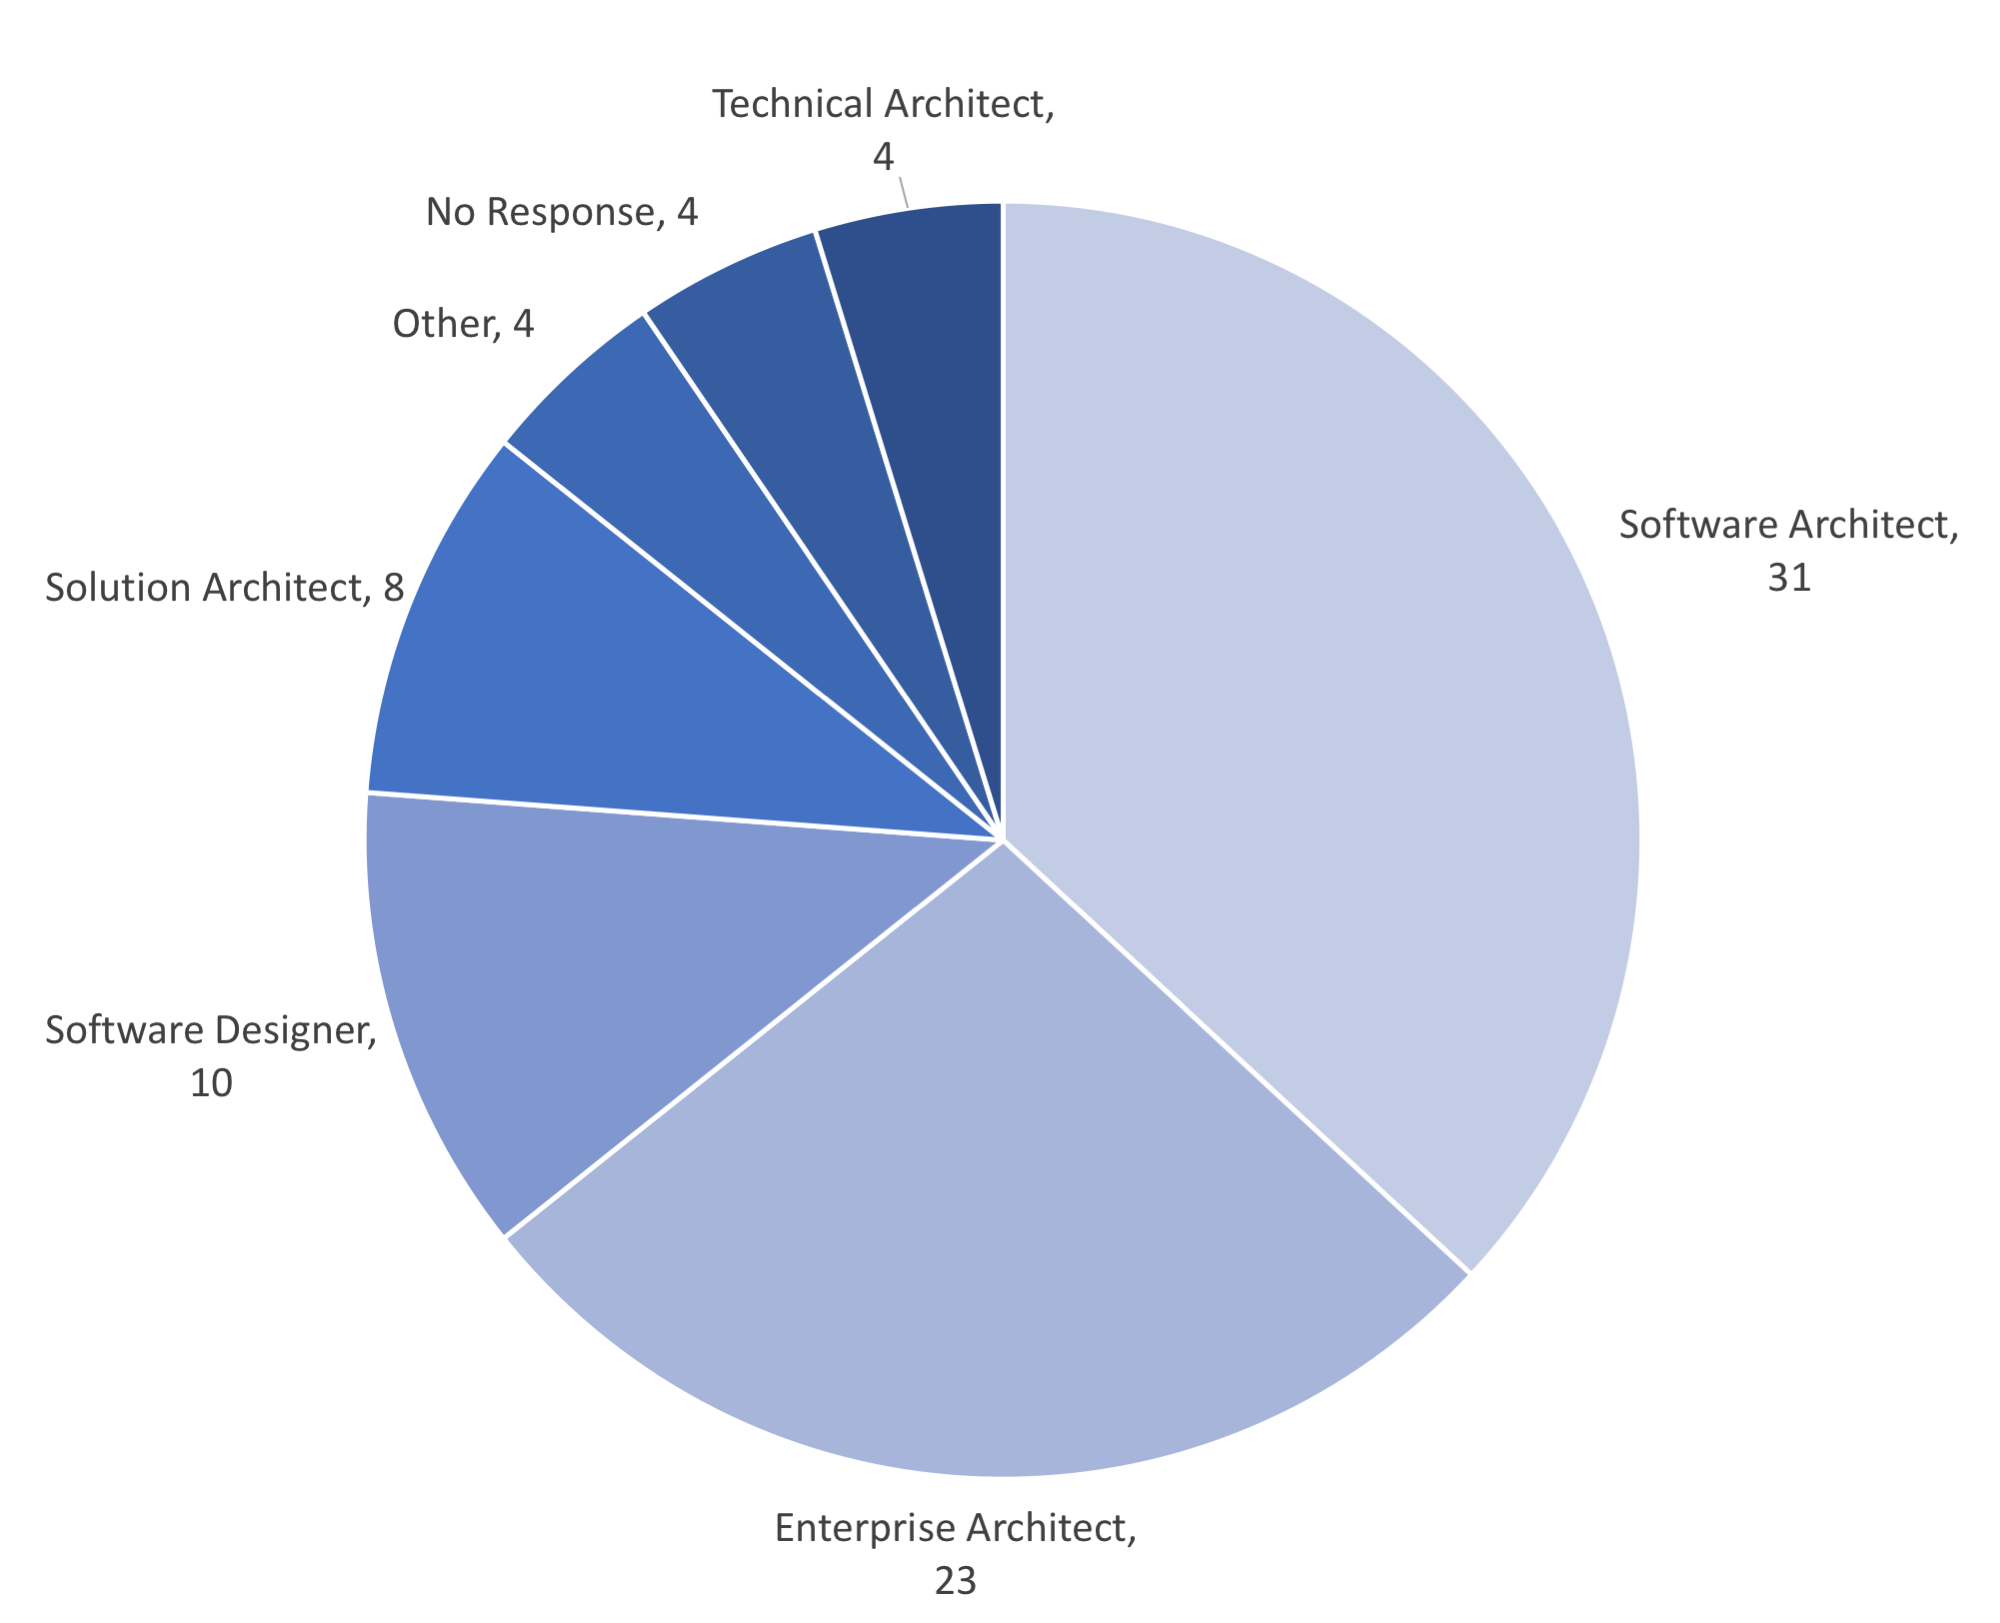
\includegraphics[width=12cm]{Figures/prioritisation-detailed-roles}
\caption{Respondent Roles}
\label{figure:resproles}
\end{figure}


The work environments of the respondents were overwhelmingly industrial (we viewed those building systems in the public sector as part of "industry"), with only one respondent having a purely academic work environment.  Five respondents did not provide an answer to this question.  Of these five, two were from German IP addresses, one Swiss and two UK addresses.  Four were from private ISP connections and one was from a UK public sector body, which, with another respondent who identified themselves as working in the public sector, suggested there were at least two public sector respondents.
 
\begin{figure}
\centering
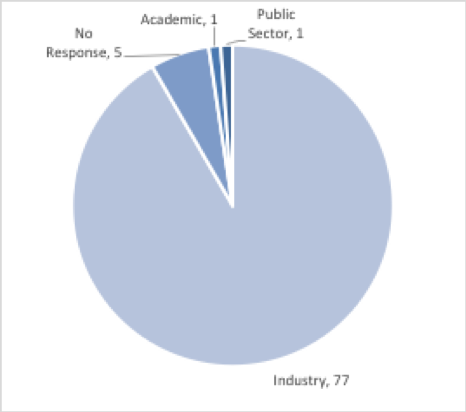
\includegraphics[width=12cm]{Figures/prioritisation-workenv}
\caption{Respondent Work Environments}
\label{figure:workenvs}
\end{figure}

We had some geographical distribution of respondents, as shown in Figure \ref{figure:geographies}, although there is a clear bias towards Europe, almost certainly caused by our professional networks being centred in Europe.  55\% of respondents identified themselves as coming from Europe, 30\% from the Americas and only 7\% from Asia-Pacific and a single correspondent from the Middle-East and Africa.

\begin{figure}
\centering
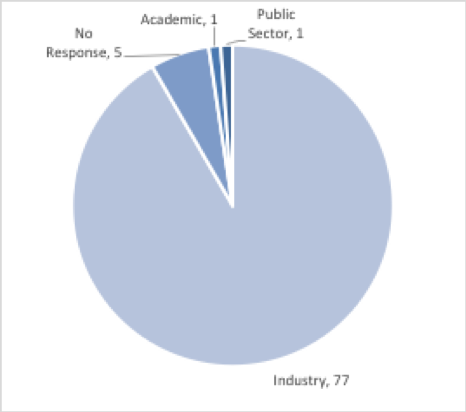
\includegraphics[width=12cm]{Figures/prioritisation-workenv}
\caption{Respondent Geographies}
\label{figure:geographies}
\end{figure}

To delve a little deeper, we checked the geographical location of the respondents' IP addresses using the well-known "geoiplookup" command line tool (http://geoiplookup.net/).  Of the four respondents who did not answer the question, the IP addresses they were using were in the UK (two), Germany (one) and Switzerland (one).  While this does not prove that the respondents work in those countries (they could have been travelling away from home) it does make it likely that they are from Europe, taking the European percentage to about 60\%.
 
\begin{figure}
\centering
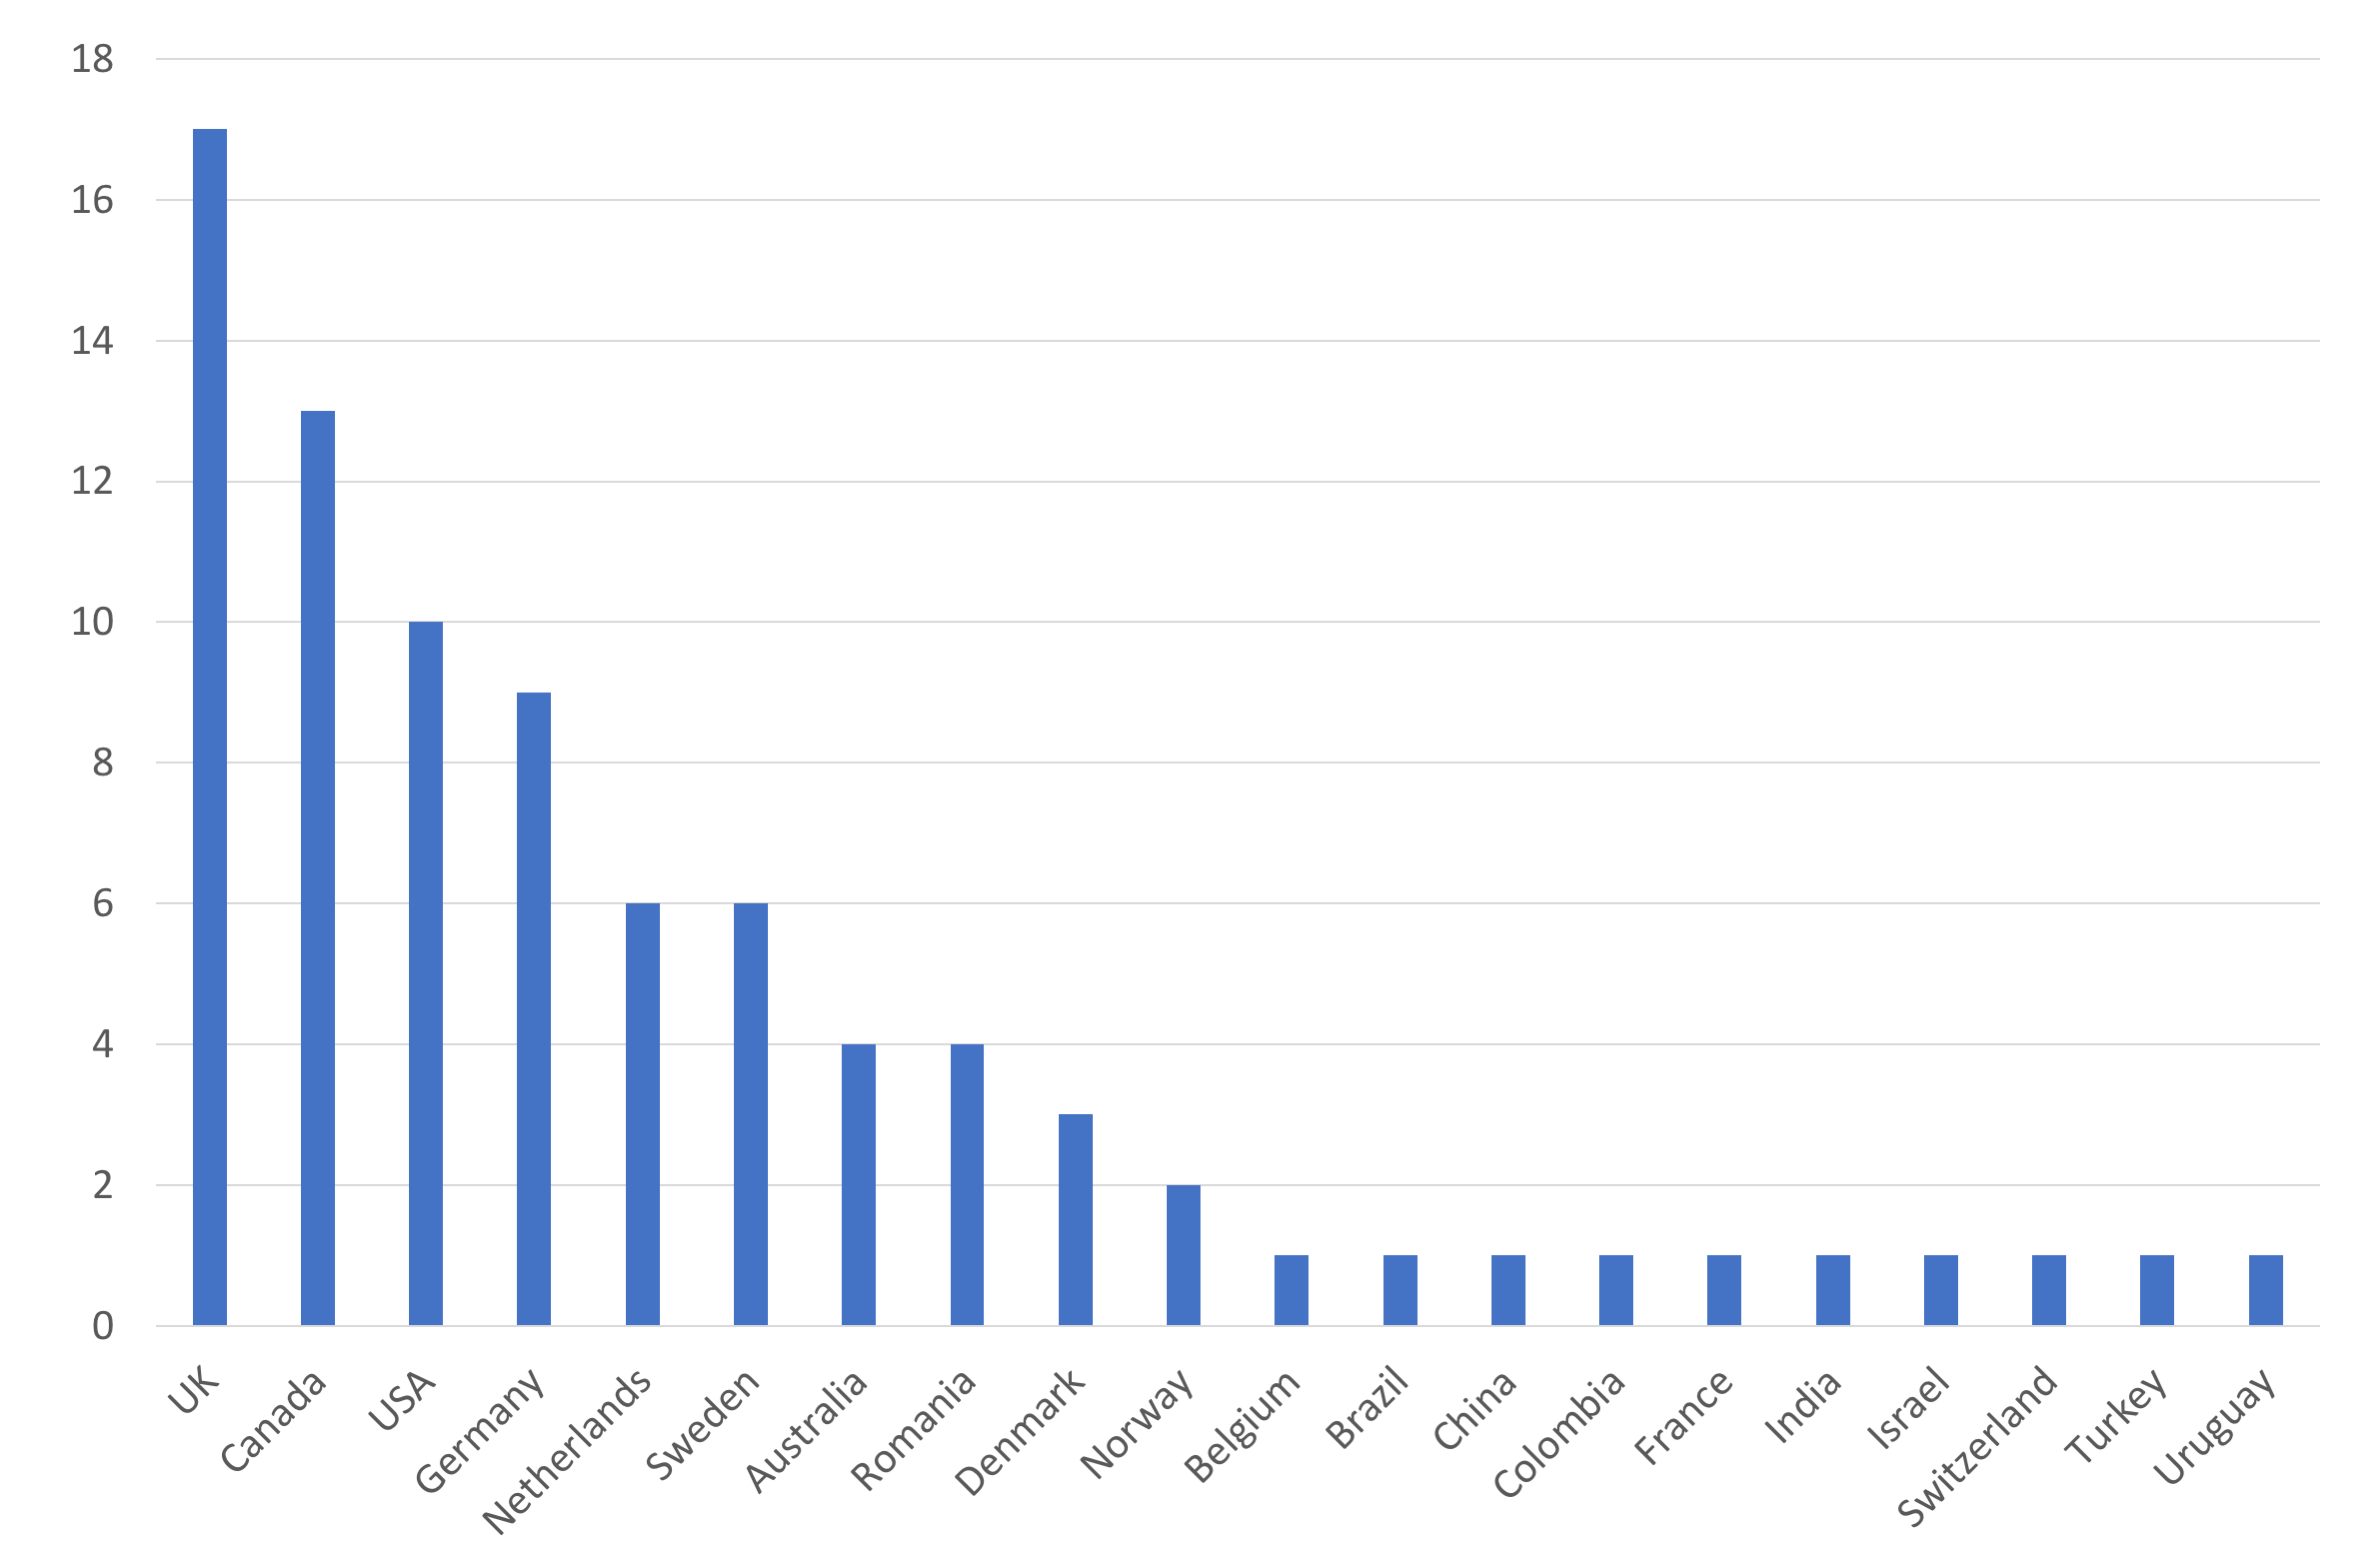
\includegraphics[width=12cm]{Figures/prioritisation-iplocation}
\caption{Respondent IP Address Locations}
\label{figure:iplocations}
\end{figure}

The result of using the respondents' IP address geographical locations to find which countries the questionnaire was completed form is shown in Figure \ref{figure:iplocations}.  While we must be cautious in assuming that these geographical locations are necessarily the locations of the respondents' homes and workplaces, it is a useful cross-check on the data.  We can see that 20 countries are represented, with 6 countries having 4 correspondents or more (which is roughly 5\% of the survey size).  These larger 6 countries are the UK, Canada, the USA, Germany, the Netherlands, Sweden, Australia and Romania.  Ten of the countries (Brasil, China, Columbia, France, India, Israel, Switzerland, Turkey and Uruguay) only had one survey completed from one of their IP addresses.  Just over 55\% of the responses were from IP addresses located in four countries, the UK (20\%), Canada (15\%), the USA (12\%) and Germany (11\%).

We discuss the possible impact of geographical location more when we consider threats to validity in section \ref{sec:threats}, but we think it is fair to say that we achieved good cross-geographic participation, but still ended up with a strong bias to Western Europe and North America.

The final classification we asked our respondents for was the number of years of experience that they had.  We asked this to ensure that participants had a significant amount of professional practice upon which to base their evaluation of the model and to allow us to understand if there are differences in the value of the model to architects with different amounts of experience.  The degree of experiences for our respondents is summarised in Figure \ref{figure:yearsexp}.
 
\begin{figure}
\centering
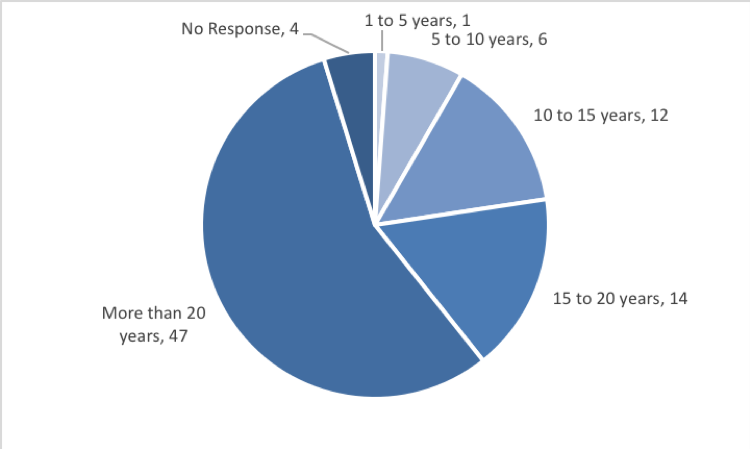
\includegraphics[width=12cm]{Figures/prioritisation-yearsexp-detailed}
\caption{Years of Experience of Respondents}
\label{figure:yearsexp}
\end{figure}

The obvious first impression is that our respondents were overwhelmingly experienced people, with over half of them (55\%) having at least 20 years of post-graduation experience.  At the other extreme only one respondent had less than 5 years of experience.  About 7\% had 5 to 10 years of experience, 15\% had 10 to 15 years and about 17\% had 15 to 20 years.  Four of our correspondents did not answer this question.

\subsection{The Results}

As mentioned earlier, we structured the questionnaire into two distinct parts, the closed-ended questions that asked people to rate the usefulness of the model and the open-ended questions that asked whether we had missed important risk areas to use with the prioritisation heuristic or whether there were any significant aspects of prioritisation that were completely missing from the model.

In this section, we review and analyse the responses for the closed-ended questions in the survey.
The first question we asked was to find out if the model was similar to how experienced architects already focused their attention, which would suggest that the model was credible and, if we assume that experienced architects are probably effective, a useful guide for less experienced architects, early in their career.  The responses we received from all of the respondents are summarised in Figure \ref{figure:similarity}.
 
\begin{figure}
\centering
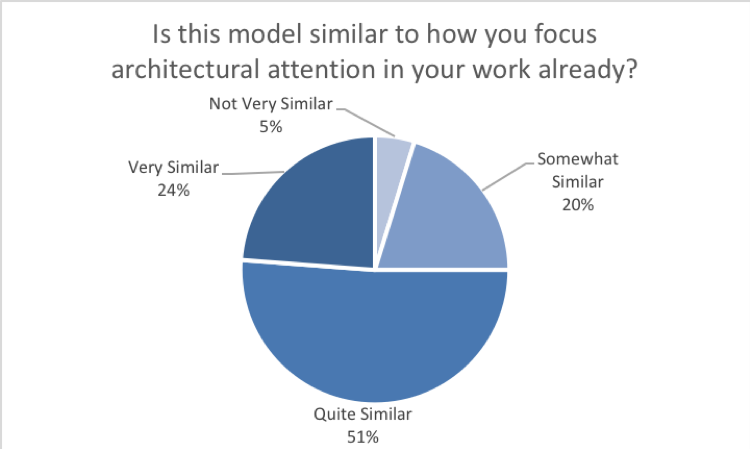
\includegraphics[width=12cm]{Figures/prioritisation-similarity}
\caption{How Similar the Model is to Existing Practice}
\label{figure:similarity}
\end{figure}

Considering all of the responses, the model validates quite strongly against the participants' existing practice, with 75\% of respondents stating that it was "very similar" or "quite similar" to their existing approach for focusing attention in their architecture work.  20\% said it was "somewhat similar", 5\% said it was not very similar to how they worked, and no respondents replied "not at all similar".

Given that we were interested in attracting experienced architects to validate the model, we were also interested in finding out whether the number of years of experience altered their view of how similar the model was to how they worked.  The summary of this information is shown in Table \ref{table:similaritybyexp}.


\begin{table}
\caption{Similarity of the Model to Practice by Experience Level}
\label{table:similaritybyexp}
\footnotesize
\begin{tabular}{l p{1.5cm} p{1.5cm} p{1.5cm} p{1.5cm} p{1.5cm}}
                & Not at All Similar & Not Very Similar & Somewhat Similar & Quite Similar & Very Similar \\
1 to 5 Years       & &          &           & 1 (100\%) &	        \\
5 to 10 Years      & & 1 (17\%) & 2 (33\%)  & 1 (17\%)  & 2 (33\%)  \\
10 to 15 Years     & & 1 (8\%)  & 3 (25\%)  & 7 (58\%)  & 1 (8\%)   \\
15 to 20 Years     & &          & 1 (7\%)   & 11 (79\%) & 2 (14\%)  \\
More than 20 Years & & 2 (4\%)  & 10 (21\%) & 22 (47\%) & 13 (28\%) \\
\end{tabular}
\end{table}

The table shows how many respondents, grouped by years of experience, rated the model at each similarity level, compared to their own approach to prioritising their work.  The 4 participants who did not indicate their experience level are excluded from this table.  The percentage values are the percentage of the participants in the current row that the value represents.

We are primarily interested in the top three groups, which is architects with at least 10 years of experience.  What we can see from this data is that the degree of similarity between the model and the architect's current practice does vary between these three groups, with 66\% of the 10 - 15 year group rating it as "quite similar" or "very similar", 93\% of the 15 - 20 years group rating it at this level and 75\% of the 20+ year group rating it in this way.  So, all three groups validate quite strongly, but it seems to reflect most strongly how the 15+ year groups work.

The second question moved on to try to establish, whether the respondents thought that model would be useful in practice.  A summary of the answers to this question across all responses is shown in Figure \ref{figure:helpfulness}.
 
\begin{figure}
\centering
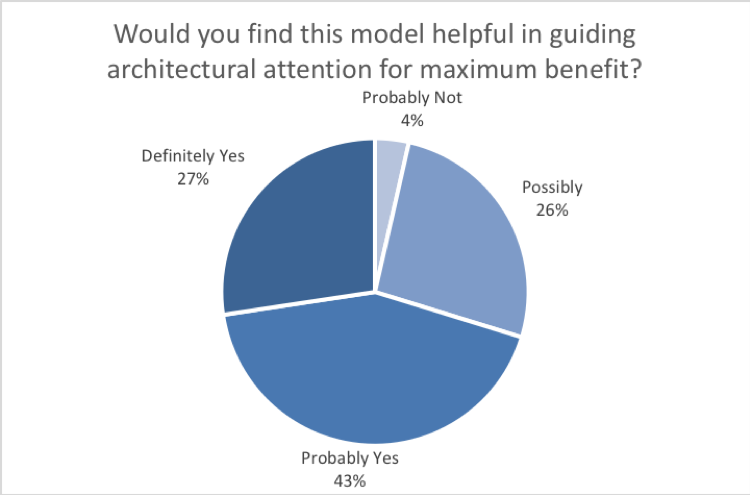
\includegraphics[width=12cm]{Figures/prioritisation-helpfulness}
\caption{Helpfulness of the Model}
\label{figure:helpfulness}
\end{figure}

Across all of the respondents, 70\% said that it was definitely or probably useful, which we interpret as a strong overall validation of the model.  The remaining respondents mainly stated that they might "possibly" find it useful.  Only 3 respondents said "probably not" and none said "definitely not".
We were interested in how the utility of the model might vary by the experience of the respondent, so we performed similar analysis by experience group to that performed for the previous question.  The results are shown in Table \ref{table:helpfulness}.

\begin{table}
\caption{Helpfulness of the Model by Experience Level}
\label{table:helpfulness}
\footnotesize
\begin{tabular}{l p{1.5cm} p{1.5cm} p{1.5cm} p{1.5cm} p{1.5cm}}
 & Definitely Not & Probably Not & Possibly & Probably Yes & Definitely Yes \\
1 to 5 Years       & &          &           &           & 1 (100\%) \\
5 to 10 Years      & & 1 (17\%) & 3 (50\%)  & 2 (33\%)  & \\
10 to 15 Years	   & &          & 4 (33\%)  & 5 (42\%)  & 3 (25\%) \\
15 to 20 Years     & &          & 4 (29\%)  & 5 (36\%)  & 5 (36\%) \\
More than 20 Years & & 2 (4\%)  & 10 (26\%) & 23 (43\%) & 12 (26\%) \\
\end{tabular}
\end{table}

Again, focusing on the architects with at least 10 years of experience, 67\% of the 10 to 15 year experience group believe the model is "probably" or "definitely" useful, 72\% of the 15 to 20 year group also rate it at this level, while 69\% of the most experienced, 20+ years of experience group, believe it is "probably" or "definitely" useful.  A strong majority of respondents in all three groups appear to find the model useful, with the strongest validation coming from the 15 - 20 years of experience group.

Finally, we wanted to check that the areas of risk we had identified as important within the "prioritise time according to risks" heuristic were valuable to a practicing architect.  The results of the corresponding question in the survey across all respondents are shown in Figure \ref{figure:validationofareas}.

\begin{figure}
\centering
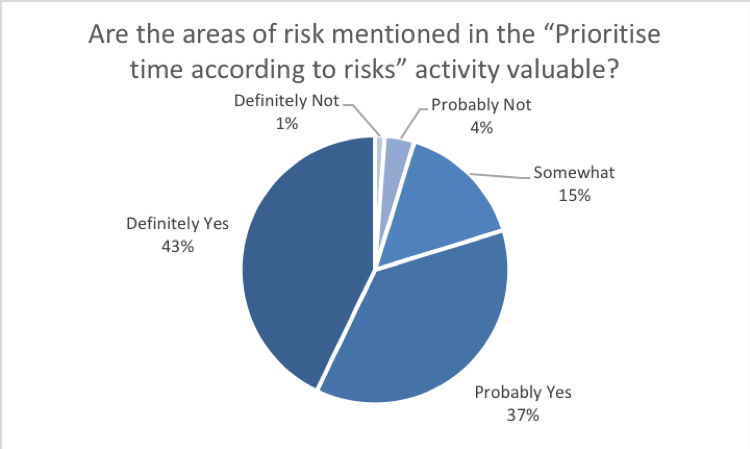
\includegraphics[width=12cm]{Figures/prioritisation-riskareas}
\caption{Validation of Risk Prioritisation Areas}
\label{figure:validationofareas}
\end{figure}

In this case we did have one very strong negative opinion ("definitely not") but this was a single individual (an enterprise architect in the 10 - 15 years of experience group, who commented in the open-ended questions that he did not believe that it was possible to define general software development risks in a useful way).

Beyond this response, 80\% of respondents believe that the areas of risk were "definitely" or "probably" valuable, suggesting that this aspect of the model should be of value to many practitioners.

Again, we analysed the responses by experience level of the respondent, which is shown in Table \ref{table:valueofriskfactors}.

\begin{table}
\caption{Value of Risk Factors by Experience Level}
\label{table:valueofriskfactors}
\footnotesize
\begin{tabular}{l p{1.5cm} p{1.5cm} p{1.5cm} p{1.5cm} p{1.5cm}}
 & Definitely Not & Probably Not & Somewhat & Probably Yes & Definitely Yes \\
1 to 5 Years       &         &          &          &           & 1 (100\%) \\
5 to 10 Years      &         & 1 (17\%) & 1 (17\%) & 2 (33\%)  & 2 (33\%) \\
10 to 15 Years     & 1 (8\%) &          &          & 5 (42\%)  & 6 (50\%) \\
15 to 20 Years     &         &          & 3 (21\%) & 6 (43\%)  & 5 (36\%) \\
More than 20 Years &         & 2 (4\%)  & 9 (19\%) & 17 (36\%) & 19 (40\%) \\
\end{tabular}
\end{table}


Looking at the architects with more than 10 years experience, we still see a high degree of validation (92\% of 10 to 15 year experience respondents, 79\% of 15 to 20 year respondents and 76\% of respondents with more than 20 years of experience saying "probably yes" or "definitely yes") but there is a larger range of opinion than before.

We had the single individual who strongly disagreed with the risk factors being valuable in the 10 - 15 year group, 3 respondents in the 15 to 20 years of experience group only feeling that they were "somewhat" valuable and 11 respondents with more than 20 years of experience stating that the factors were "somewhat" or "probably not" valuable.

This said, we still feel that the degree of validation that the model received across all of the experience levels indicates that the model has a high possibility of being useful to at least a majority of practitioners.

We were also interested to investigate if the key question of how useful the model was would vary significantly between our different respondent groups, particularly by job family and geography, which might suggest that the model aligned better with certain types of architecture work or practice in certain parts of the world.

We have analysed the responses to the question "Would you find this model helpful in guiding architectural attention for maximum benefit?" by role type and the results are shown in Table \ref{table:usefulnessbyrole} and Figure \ref{figure:usefulnessbyrole}.

\begin{table}
\caption{Usefulness of the Model by Role Type}
\label{table:usefulnessbyrole}
\footnotesize
\begin{tabular}{l p{1.5cm} p{1.5cm} p{1.5cm} p{1.5cm} p{1.5cm}}
 & Definitely Not & Probably Not & Possibly & Probably Yes & Definitely Yes \\
Software Architect	 &  &  1 (3\%)  & 11 (35\%) & 13 (42\%) & 6 (19\%) \\
Software Designer    &  &  1 (10\%) & 2 (20\%)  & 5 (50\%)	& 2 (20\%) \\
Solution Architect   &  &           & 2 (25\%)  & 5 (63\%)  & 1 (12\%) \\
Technical Architect	 &  &           &           & 2 (50\%)  & 2 (50\%) \\
Enterprise Architect &  & 1 (4\%)   & 4 (17\%)  & 9 (39\%)  & 9 (39\%) \\
\end{tabular}
\end{table}

\begin{figure}
\centering
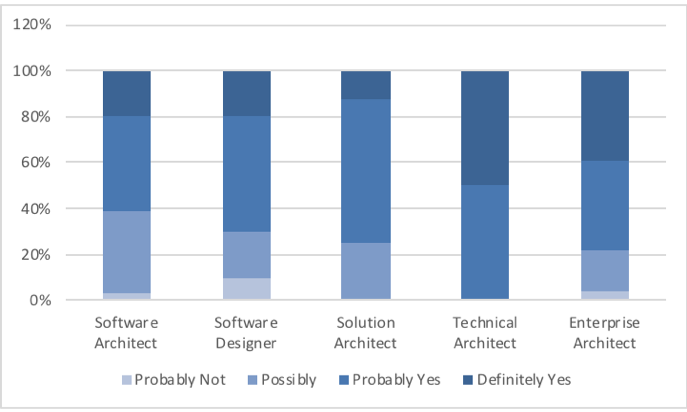
\includegraphics[width=12cm]{Figures/prioritisation-usefulness-by-role}
\caption{Usefulness of the Model by Role Type}
\label{figure:usefulnessbyrole}
\end{figure}

As can be seen, all of the respondent role groups validated the model as "probably" or "definitely" useful, with the lowest validation (interestingly) coming from the Software Architect group, where 61\% of the respondents indicated this level of agreement (although nearly all of the remaining respondents were neutral - "possibly" - rather than negative).  In the Software Designer group 70\% of respondents, in the Solution Architect group 75\%, in the Technical Architect group 100\% and in the Enterprise Architect group 78\% of respondents considered the model to be "definitely" or "probably" useful.

Turning to the possible influence of geographical location, we analysed the same question as to the usefulness of the model by the respondents, by the geographical location that the respondents told us they were from.  The results are summarized in Table \ref{table:usefulnessbygeo} and Figure \ref{figure:usefulnessbygeo}.

\begin{table}
\caption{Usefulness of the Model by Geography}
\label{table:usefulnessbygeo}
\footnotesize
\begin{tabular}{l p{1.5cm} p{1.5cm} p{1.5cm} p{1.5cm} p{1.5cm}}
% slightly experimental bit here - aligns headers centrally and leaves the
% others with default alignment from the definition above
% https://tex.stackexchange.com/questions/2924/how-to-align-table-headers-differently-than-all-other-table-cells
 & \centering Definitely Not & 
   \centering Probably Not & 
   \centering Possibly & 
   \centering Probably Yes & 
   \centering Definitely Yes \tabularnewline
Americas              & &         & 6 (23\%)  & 10 (38\%) & 10 (38\%) \\
Asia-Pacific          & &         & 3 (50\%)  & 3 (50\%)  & \\
Europe (inc. UK)      & & 3 (6\%) & 11 (23\%) & 22 (45\%) & 11 (23\%) \\
Middle-East \& Africa & &         & 1 (100\%) &           & \\
\end{tabular}
\end{table}
 
\begin{figure}
\centering
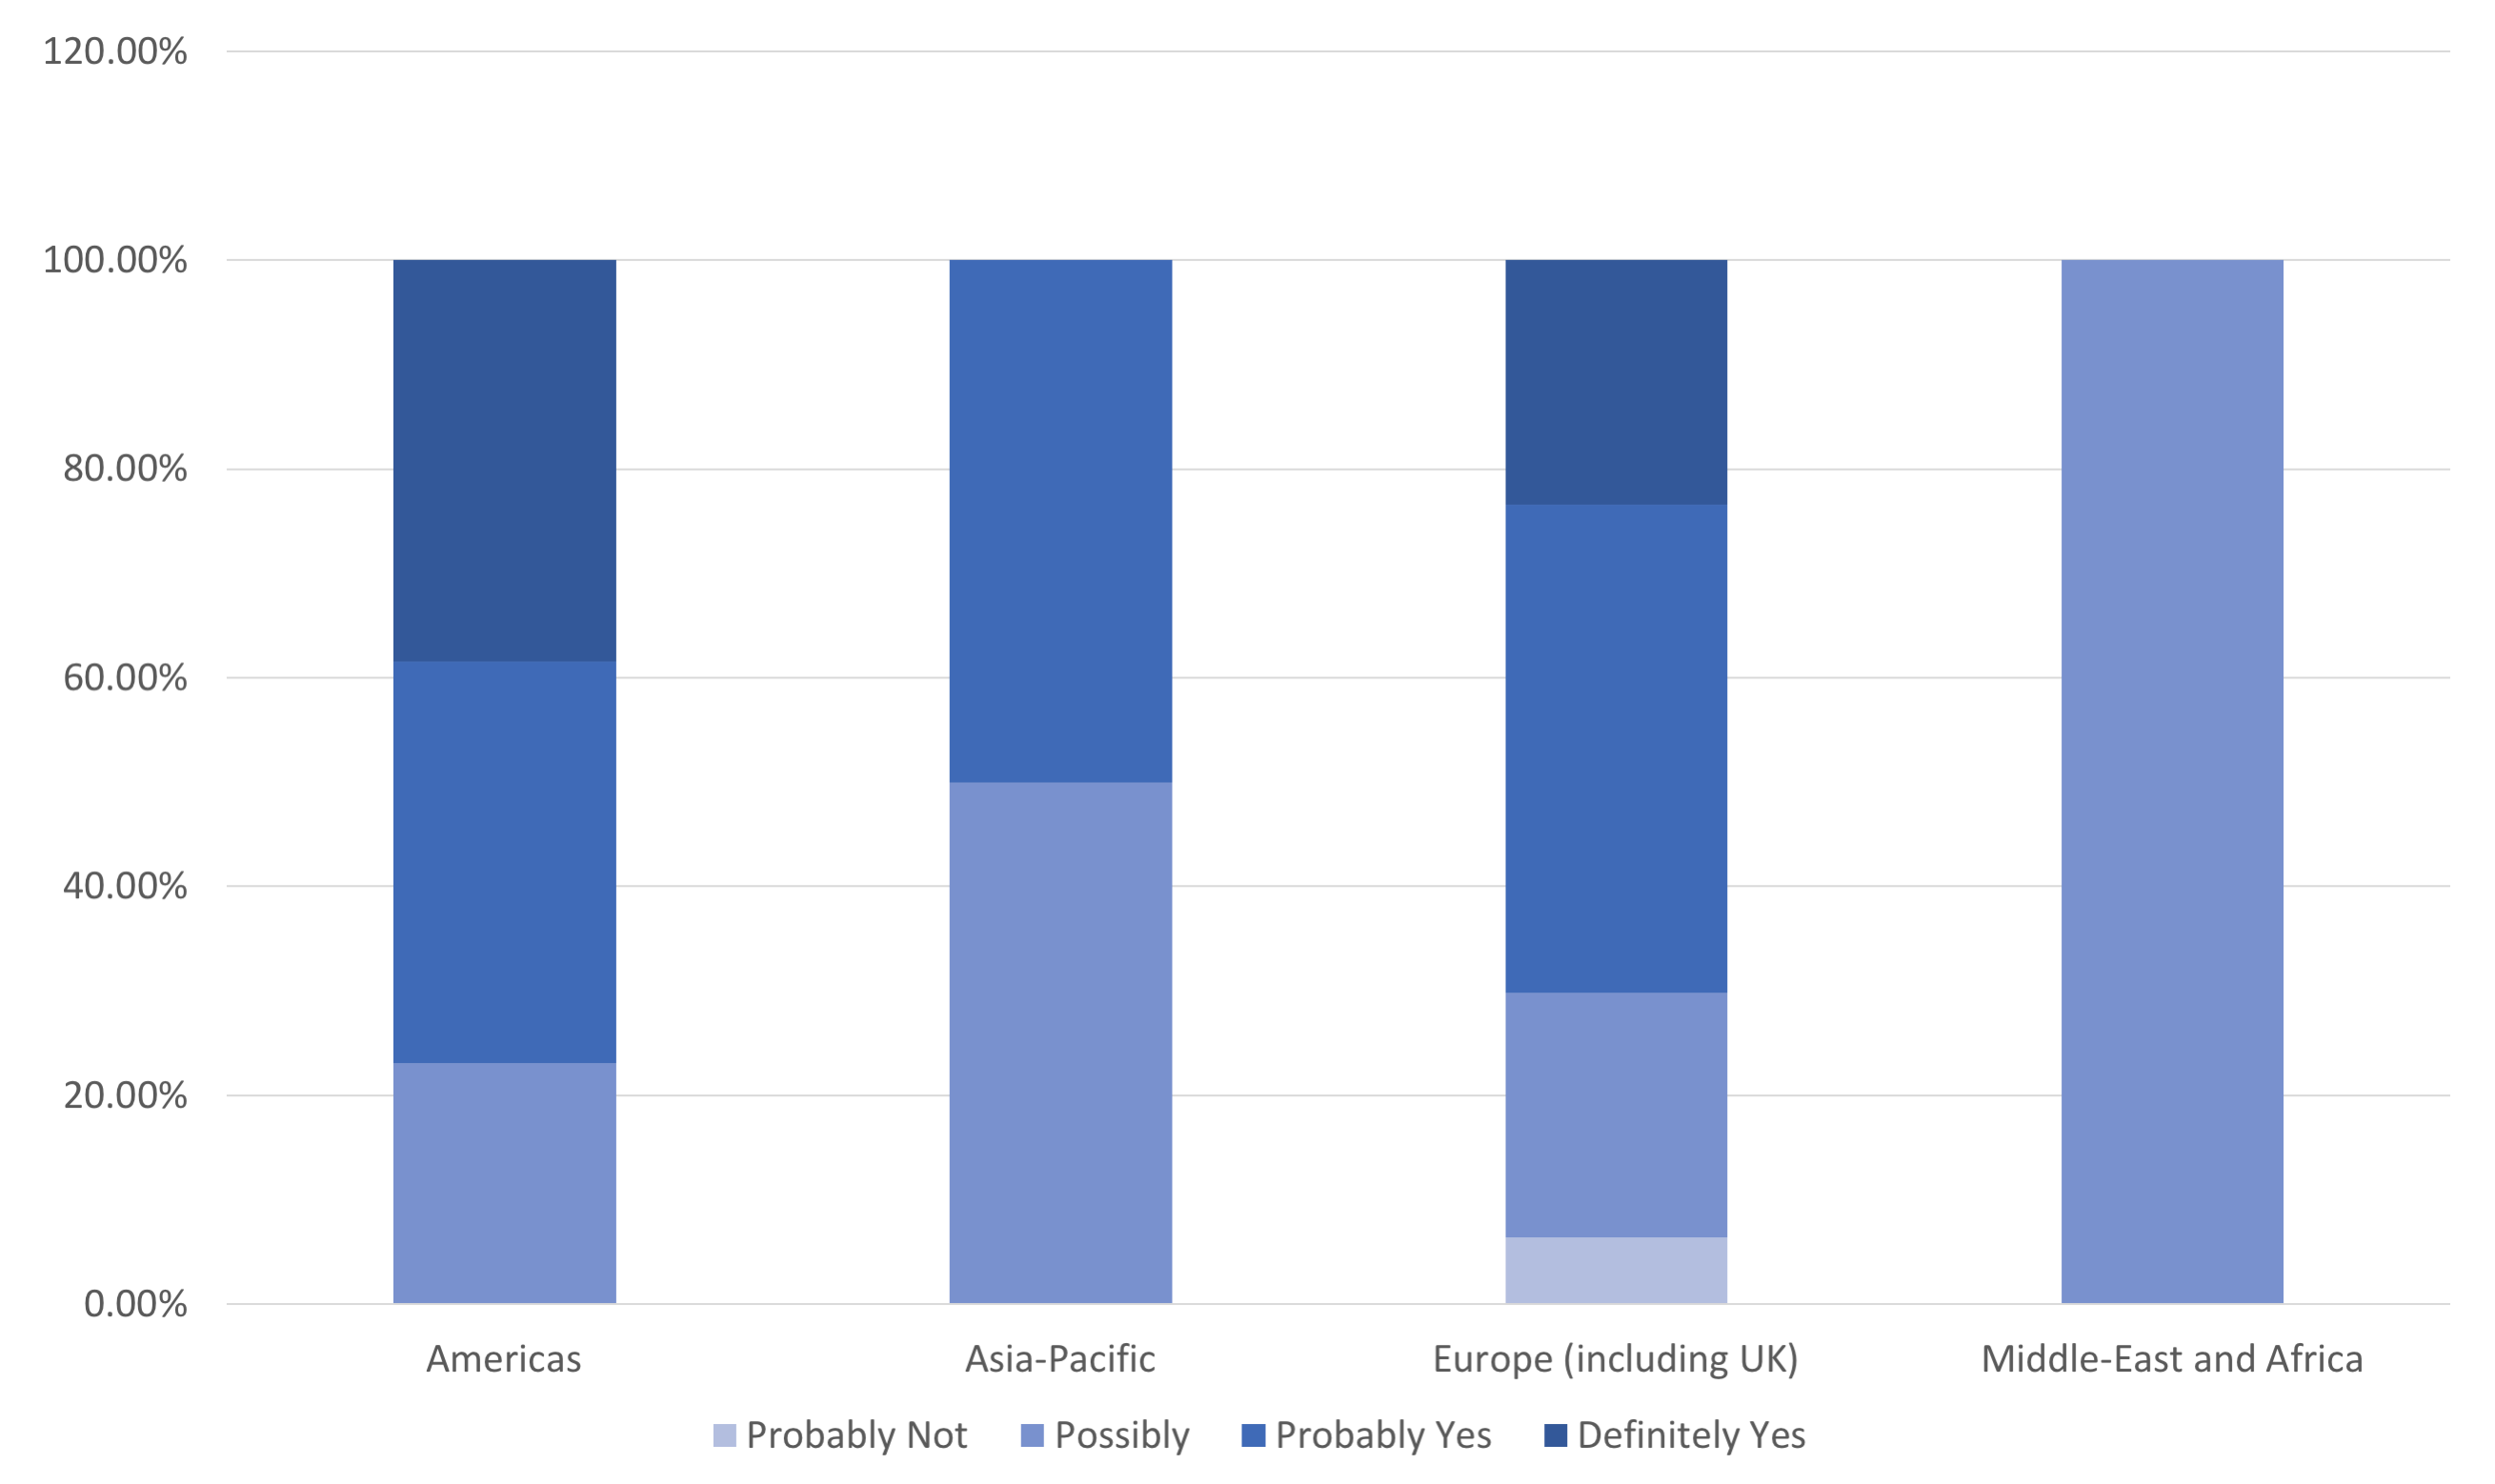
\includegraphics[width=12cm]{Figures/prioritisation-usefulness-by-geo}
\caption{Usefulness of the Model by Geography}
\label{figure:usefulnessbygeo}
\end{figure}

In this analysis we have included all of the regions, but in reality the data for the Middle-East and Africa and Asia-Pacific is difficult to use with confidence as there were very few respondents from these regions (1 from ME\&A and 6 from APAC).  Therefore, while recognising the importance of these regions and their contribution to contemporary software engineering, we focus on Europe and the Americas for the purposes of this specific analysis.

We had 26 respondents from the Americas and 69 from Europe (including the UK).  Both of these contributions are large enough to be significant, being 31\% and 82\% of the total responses, respectively.

Of these significant geographical groups, the group from the Americas validated the usefulness of the model more strongly, with 76\% of respondents indicating that the model was "definitely" or "probably" useful.  For the European group, 68\% of the respondents indicated that the model was "definitely" or "probably" useful.

We interpret this data as suggesting that the model validates well in both the Americas and in Europe and should be useful in both regions.  The data we have suggests that it should also be useful in Asia-Pacific as 50\% of respondents indicated it would be useful, while in contrast it may not be useful in ME\&A as our single respondent from that region indicated it was "probably not" useful; However, we do not have enough respondents from these regions to draw meaningful conclusions.  To investigate the usefulness of the model in APAC and the Middle-East and Africa would require a further study.

In summary, having analysed the answers to the closed-ended answers in our survey, we conclude that our model is likely to be credible and useful in Europe and the Americas and broadly aligns with the prioritisation approach used by many experienced architects in those regions.
We view this as a successful validation of the model; However, we were also interested in how the model could be improved and so we used the responses to the open-ended questions in the survey to find themes which we could include in a refined model.

\subsection{Analysing the Open-Ended Responses}
\label{sec:openended}

As explained earlier, we asked two important open-ended, questions, Q4, to identify missing risk factors from the "prioritise time according to risks" heuristic ("are there other general areas of risk that should be added to "prioritise time according to risks" that would be applicable to most (information) systems and environments?") and Q5, to ask whether we had missed any important aspect of the model entirely ("are there any significant factors missing from the model which you use to focus your architectural work?").

We had 44 responses to Q4, about missing aspects of the model, and 51 responses to Q5, about missing areas of risk.

Given the nature of these responses, we again used grounded theory style analysis to analyse them, coding each one initially using straightforward, descriptive labels, directly reflecting the language used in the response, then refining this with further coding steps, to identify higher-level categories to allow the responses to be collected into meaningful groups.

For the first question, Q4, we initially coded the responses to 37 distinct categories, plus two null categories for the initial coding of "None" and "General Comment" for those responses which were present but did not specify a new risk area or just made a general comment.  The responses suggested a diverse range of possible risk areas, and when we refined the coding to find common concepts, this resulted in 24 higher level categories.  We attempted to refine this further but did not find further meaningful refinements as we tried further rounds of coding (we judged that we had reached "theoretical saturation" with the data).   In addition, we had a very long "tail" of concepts with only a single mention in the responses, leaving us with 5 categories that had 4 responses or more: Organisational Environment (11 occurrences), Stakeholders (6 occurrences), Cost (6 occurrences), Time (4 occurrences), External Environment (4 occurrences).  We chose to focus on categories with at least 4 occurrences as this represents approximately 5\% of the total respondents to the survey and we judged this to be high enough to warrant consideration.

In the context of a survey with over 80 responses, none of the categories of response for missing risk factors was universally viewed as important, but we felt that it was important to reflect the fact that these four factors had been independently identified by a number of people.  Therefore, we decided to integrate these new factors into the refined version of the model.

For the second open-ended question, Q5, on missing aspects of the model, we initially coded the responses into 43 distinct categories, again plus "None" and "General Comment".  As we continued with the process of refining the coding further, we ended up with 26 higher level categories.  As with the responses to Q4, many of the categories were only mentioned once and only four were mentioned 4 times or more: Team Effectiveness (10), Benefits (7), Stakeholders (6) and Time (5).  Of these factors, "Stakeholders" are already a significant factor in the model and the comments provided in these cases were suggesting a particular emphasis on certain stakeholders or method of dealing with stakeholders.  The specific suggestions were all different and stakeholder needs and priorities are already a significant part of the model, so we did not feel that a new model element was needed, but we simply need to review the detailed comments and ensure that they are reflected in the existing elements of the model.

In this context, we felt that adding a completely new aspect to the model was a significant step and so we only wanted to consider this for aspects which had been identified as important by a significant number of respondents to the survey.  On this basis, we decided to add a new element to the model to reflect the "Team Effectiveness" theme as it was the only additional candidate aspect that at least 10\% of the respondents had identified as important.

Finally, we also received 37 general comments in the open-ended question at the end of the survey along with another 14 responses to the other open-ended questions which we judged to be general comments rather than specific answers to those earlier questions, making a total of 51 general comments.  We do not view these responses as part of the validation of the model, but some of them did provide useful commentary on the work.  Again, we used a grounded theory style coding approach to analyse the data and this resulted in 23 categories of comment.  Like the other open-ended questions, most of these categories were not judged as significant because less than four respondents mentioned them.

The categories which had four or more respondents were general Positive Comments such as "nice and simple model" (14), comments on the How the Architect Should Work, such as "an architect must help implement what he/she helped to decide" (6) and comments on the Presentation of the Model, such as "this model […] does appear to be a rather linear, and distinct,  in reality it [the process] is quiet (sic) iterative and overlapping" (5).

We found all of the general comments interesting and potentially useful, but most of them did not lead us to conclude that further changes were needed to the model.  The exception was the group of comments categorised as Presentation of the Model.  These 5 comments suggested that the respondents interpreted our graphical presentation of the model as indicating a linear "upfront" process.  In fact, we had meant to communicate exactly the opposite through our diagram, and indicate that the process is iterative and continuous, happening right through the project's lifecycle.  We took this as an important indicator that we needed to change the graphical representation of the model and also describe its intended iterative and continuous nature more clearly in the supporting text.

\section{Stage 4 - The Refined Model for Prioritising Architectural Effort}

We took the outputs of the open-ended question analysis described in section \ref{sec:openended} and used them to add missing features of the model, improve the list of risks to suggest for time prioritisation and improve the model using the advice provided in the general comment responses to the survey.
The result of these additions is a refined model for prioritising architectural effort, with an additional feature of the model, "Team Effectiveness" and a refined list of risks for time prioritisation.  As mentioned earlier, we also decided to alter the graphical presentation of the model to try to emphasise that it is not a linear "process" but rather a set of activities to be performed throughout the project lifecycle.  The refined model is shown in Figure \ref{figure:refinedmodel}.

\begin{figure}
\centering
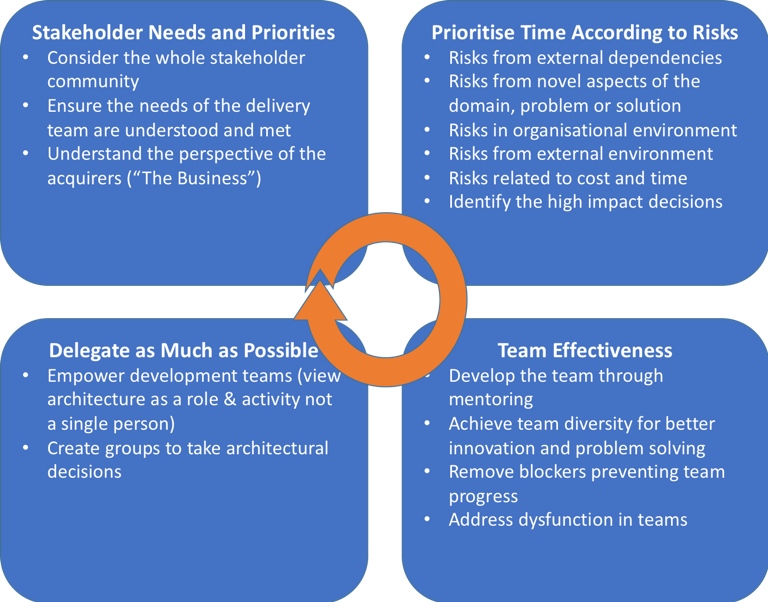
\includegraphics[width=12cm]{Figures/prioritisation-refined-model}
\caption{Refined Model for Prioritising Architectural Attention}
\label{figure:refinedmodel}
\end{figure}

The model is comprised of 4 aspects, Stakeholder Needs and Priorities, Prioritise Time According to Risks, Delegate as Much as Possible and Team Effectiveness.  Each aspect is a theme which our initial interviewees and the later survey respondents find useful when considering how to prioritise their architectural work.  The details of each theme are described in the subsections below. 

The idea of the model is to provide a guide for new architects, or an aide-memoir for experienced architects, on how to prioritise their architectural work in order to maximise its effectiveness.  It is not a process or a step to be followed in an architectural "method" but rather these are themes for effective effort prioritisation that should be repeatedly considered during the lifecycle of a project.
As with any set of heuristics, they can only be a generalised starting point and need to be considered, interpreted and applied in a context specific way by the architects and teams who use them.  However, they have validated well against a reasonably broad survey of experienced, practicing architects and so we believe that they are a useful starting point upon which to build a personal approach for prioritisation.

\subsection{Stakeholder Needs and Priorities}

The first theme which emerged strongly in our study was focusing on the needs and priorities of the stakeholders involved in the situation.  The principle that architecture work involves working closely with stakeholders is widely agreed \cite{rozanski2011-ssa2e, bass2012-sainp} and this theme reinforces that. Architects need to focus significant effort to make sure that stakeholder needs and priorities are understood to maximise focus on the critical success factors for a project and maximise the chances of its success.  Three specific heuristics to achieve this which emerged from the study are:

\begin{itemize}
	\item \emph{Consider the whole stakeholder community}. Spend time understanding the different groups in the stakeholder community and avoid the mistake of just considering obvious stakeholder groups like end-users, acquirers and the development team.  As the architecture methods referenced above note, ignoring important stakeholders (like operational staff or auditors) can prevent the project meeting its goals and cause significant problems on the path to production operation.
	\item \emph{Ensure that the needs of the delivery team are understood and met}.  Spend sufficient time to ensure that the delivery team can be effective.  What is the team good at?  What does it know?  What does it not know?  What skill and knowledge gaps does it have?  These areas need attention early in the project so that architecture work avoids risks caused by the capabilities of the team and that time is taken to support and develop the team to address significant weaknesses.
	\item \emph{Understand the perspective and perceptions of the acquirers of the system}.  Acquirers are a key stakeholder group who judge its success and usually have strategic and budgetary control, so can halt the project before delivery if they are unhappy.  Specifically addressing this group's needs, perceptions and concerns emerged as an important factor for some of the experienced architects in our study.  Acquirers are often senior managers and so may be distant from the day-to-day reality of a project and need regular, targeted, clear communication to understand their concerns and ensure that they have a realistic view of the project. 
\end{itemize}

\subsection{Prioritise Effort According to Risks}

During a project, an effective approach to prioritising architectural attention is to use a risk-driven approach to identify the most important tasks.  If the significant risks are understood and mitigated, then enough architecture work has probably been completed.  If significant risks are open, then more architecture work is needed. The specific heuristics to consider for risk assessment are:

\begin{description}
	\item \emph{Risks from external dependencies}.  Understand your external dependencies because you have little control over them and they need architectural attention early in the project and whenever things change.
	\item \emph{Risks from novel aspects of the domain, problem or solution}.  Another useful heuristic, from the experience of our study participants, is to focus on novelty in your project.  What is unfamiliar?  What problems have you not solved before?  Which technology is unproven? The answers to these questions highlight risks and the participants in our study used them to direct their effort to the most important risks to address.
	\item \emph{Risks in organisational environment}.  Each organisation is different and there are nearly always risks specific to an environment such as the internal political situation, what is possible in the organisational culture, and the maturity of the organisation with respect to architecture, change and risk.  Different organisations also have different cultures and capabilities for funding change, which can create risks.  The speed which different sorts of risk and difficulties can be addressed can also be affected by organisational factors and so may cause you to change where you focus attention.  Participants in our study noted the importance of "situational awareness" \cite{wikipedia-sitawareness} that allows the architect to find and address the risks specific to their organisational environment.
	Risks from external environment.  Nearly all organisations exist in a complex ecosystem of interacting partners, customers regulators, competitors and other actors and they can be a source of risk for many systems, as can general trends and changes in the industry that the organisation exists within (such as changing regulatory environment or industry-wide pressures such as reducing margins on products or services). 
	\item \emph{Risks related to cost and time}.  Most architects will report that they are often expected to achieve challenging goals in unrealistic timescales or with unrealistic cost estimations.  Many of our study participants reported that they needed to focus significant attention on risks resulting from cost and time.
	\item \emph{Identify the high impact decisions}.  Prioritise architecture work that will help to mitigate risks where many people would be affected by a problem (e.g. problems with the development environment or problems that will prevent effective operation) or where the risk could endanger the programme (e.g. missing regulatory constraints).
\end{description}

\subsection{Delegate as Much as Possible}

Delegation was an unexpected theme that emerged from our study. The architects who mentioned this theme viewed themselves as a potential bottleneck in a project and delegation and empowerment of others was a way to minimise this.  Delegation was also seen as a way of freeing the architect to focus on the aspects of the project that they had to focus on rather than all the other aspects that they could possibly get involved in.

The general message of this theme is to delegate as much architecture work as possible to the person or group best suited to perform it, to prevent individuals becoming project bottlenecks, allow architects to spend more time on risk identification and mitigation, and to spread architectural knowledge through the organisation.  The heuristics that were identified to help achieve this are:

\begin{description}
	\item \emph{Empower the development teams}. To allow delegation and work sharing, architects need to empower (and trust) the teams that they work with.  This allows governance to become a shared responsibility and architecture to be viewed as an activity rather than something that is only performed by one person or a small group.  This causes architectural knowledge, effort and accountability to be spread across the organisation, creates shared ownership, reduces the load on any one individual and prevents reliance on a single individual from delaying progress.
	\item \emph{Create groups to take architectural responsibilities}.  A related heuristic is to formalise delegation somewhat and create groups of people to be accountable for specific aspects of architectural work.  For example, in a large development programme, an architecture review board can be created to review and approve significant architectural decisions.  Such a group can involve a wide range of expertise from across the programme and beyond, so freeing a lead architect from much of the effort involved in gathering and understanding the details of key decisions, while maintaining effective oversight to allow risks to be controlled and technical coherence maintained.  Similarly, a specific group of individuals could be responsible for resilience and disaster recovery for a large programme, allowing them to specialise and focus on this complex area, and allowing a lead architect to confidently delegate to them, knowing that they will have the focus and expertise to address this aspect of the architecture.
\end{description}

\subsection{Team Effectiveness}

A theme that emerged when we validated our initial model with a wider group was the need to focus attention on making sure that the overall development team was as effective as possible.  The participants who indicated the importance of this factor were concerned with the need to develop the individuals in the team and to ensure that the team was as diverse as possible, to allow it to use a range of skills and perspectives when innovating and solving problems.

Other aspects of this theme that participants were concerned with were the importance of architecture work being used to quickly unblock the team when it hit difficulties and the importance of technical leaders, like the architect, to step in when needed to make sure that the team was functioning well and to address any dysfunctional behaviour observed.

The heuristics that the participants identified as being important for focusing architectural attention to achieve team effectiveness were:
\begin{description}
	\item \emph{Develop the team through mentoring}.  Every team should be on a collective journey towards improvement and hopefully every individual in a team is on a similar personal journey to be the best that they can be.  People doing architecture work tend to be some of the most experienced people in a team and so a valuable and important area to focus attention, in order to achieve a highly effective team, is to spend time developing the individuals in the team, and the team as a whole, through thoughtful, intentional mentoring.
	\item \emph{Achieve team diversity for better innovation and problem-solving}.  In order to innovate and identify good solutions to problems, it is valuable to have a range of experience, perspectives and skills in the team.  Our study participants indicated that a valuable use of architectural time is to spend time building diverse teams that can achieve this.
	\item \emph{Remove blockers preventing team progress}.  Development and support teams often tend up blocked by technical or organisational factors, so spending time resolving these problems is a valuable focus for many architects.
	\item \emph{Address dysfunction in teams}.  Sometimes teams do not work well and it requires someone who is close to the team, and respected by them, but outside the team structure, to identify the problem and suggest solutions.  Some architects work directly in individual teams and are not well placed to do this, but people doing architecture work are often close to the teams but outside their structure, and have the respect, soft-skills and experience to resolve team problems.  This use of architectural time can have huge benefits when dysfunctional behaviour is observed in teams.
\end{description}

\section{Threats to Validity}
\label{sec:threats}

We designed and conducted this study carefully to provide us with a useful model and a reliable evaluation of it, avoiding bias as much as possible.  Specific steps we took to produce a reliable evaluation of the model included focusing on the practitioner community (as they are the intended users of the model), focusing on experienced respondents who have the experience to evaluate the model, finding a reasonably large, geographically distributed group to validate it for us, structuring the questionnaire to allow disagreement as well as confirmation, and analysing the results in a careful, structured manner to allow the data to lead us to the conclusions, to avoid the danger of us subconsciously using it to validate an opinion we already held.  However, we acknowledge that there are potential limitations to any qualitative study, including ours, which can result in threats to our study's validity.

There are four main types of threat to the validity of a study like this, namely construct, internal, 
external and conclusion validity as defined in \cite{matt1994-threatstovalidity}. 

Construct validity is concerned with the relationship between theory and observation.  A commonly recurring threat when using questionnaires is the phrasing of the text, the questions and the responses for the closed-ended questions.  A second threat is where too many closed-ended questions are used and respondents cannot find suitable responses in the set that are available.  We addressed potential problems with wording by keeping the amount of text in the questionnaire as small as possible and using simple language that directly referenced the model.  The model itself was derived from the language and concepts that emerged from the semi-structured interviews.  We also tested the questionnaire ourselves and on a small number of other architects that we knew, to ensure that their interpretation of the questionnaire was as we expected and we refined the language slightly as a result.  We mitigated the possible problem of participants being unable to express their opinions through the closed-ended questions by limiting the closed-ended questions to being simple ratings and then providing open-ended questions for the participants to explain, expand or clarify their answers.

Internal validity is concerned with the validity of the causality relationship between the observations and the outcomes of the study.  We addressed this by using very straightforward analysis approaches, both for the statistical data analysis and for the analysis of open-ended answers, so the threats to the correctness of the analysis we performed are minor.  We also reviewed all of the answers from each respondent to ensure that they formed a credible and consistent set (which all did), so validating that the respondents understood the process and were expressing a coherent opinion.  To avoid possible misunderstanding we provided a clear definition of the model, links to additional information, trialled the questionnaire with people we knew, and included open-ended questions to allow respondents to express opinions that could not be easily captured using the closed-ended questions.

External validity is concerned with the generalisability of the results of the study.  The key risk we identified relating to external validity is an unrepresentative respondent population or a respondent population who lack competence in software architecture and so cannot validate the model effectively.  We mitigated these risks by finding a relatively large respondent population, who are distributed geographically, although as noted earlier, nearly all of the respondents came from Europe and the Americas.  So a residual risk we continue to have is the lack of representation from Asia, in particular countries like India, China and Singapore, with significant software engineering populations and the potential for significant cultural differences from Europe and the Americas.  We mitigated the concerns around experience and competence by targeting experienced architects and architects in our extended professional network, who we knew to be experienced and highly competent.  We know a significant percentage of the respondents at least slightly and through some informal sampling of employing organisations and job titles, have a high degree of confidence in the ability of our study participants to validate or critique the model correctly.  This leaves us with a residual risk that our extended network may be more likely to think similarly than a truly random sample, but anecdotally we do not believe that they are significantly different to most practitioners we have met over the years and we believe this trade-off to ensure credible study participants is the correct one.

Conclusion validity is concerned with the validity of the relationship between the data obtained in the study and the conclusions that have been drawn from it.  The threats that we identified in this area are whether we asked the right questions at each stage of the study, whether we made mistakes in analysing the data, and whether we introduced unconscious bias into the study which could invalidate our conclusions.  We mitigated the possibility of asking the wrong questions by using a semi-structured interview in the first stage and providing extensive opportunity for open-ended responses in the third stage.  We acknowledge that we could have made mistakes in our analysis and processing of the data, but we mitigated this by reviewing and cross checking our work and using a simple, repeatable process which was straightforward to follow.  The largest risk to conclusion validity is probably the chance of introducing unconscious bias, as much of the study involved interpreting open-ended responses from the interviews and the questionnaire.  We attempted to mitigate this risk through the use of the grounded theory process, which helped us to be led by the data rather than trying to fit the data into a pre-existing theory.  We also reviewed our conclusions several times and repeated parts of the analysis if we felt that there was any danger of an alternative outcome being more representative.  We also did not have any preconceived ideas about the likely outcome of this study at the beginning, so did not have an underlying theory we were trying to validate.  Overall, we do not feel that we have been likely to introduce unconscious bias in the study, but we accept that it is hard to be certain that this did not occur at all.

In summary, we have designed and executed the study carefully, but do acknowledge that there are a number of threats to its validity which could threaten the generalisability of our results.  Probably the most severe threat to global applicability of the model is the lack of study participants from Asia.  However, this threat does not suggest that the model will not be useful in Europe and North America, which would still be a very valuable outcome.

\section{Conclusion}

Our experience and informal discussion with architects over many years suggested that they find it difficult to decide how to focus their effort to maximise their effectiveness.  We were interested in how experienced practitioners solved this problem and whether there were commonly used heuristics.  To investigate this, we used a four-step process of investigation.

We started with a semi-structured interview process with eight experienced practitioners.  The conclusion of the initial study was that there are some shared heuristics which practitioners use, but that the community of practicing architects is not aware that the heuristics are common and shared.  We found that the heuristics clustered into three groups: focus the architects attention on stakeholders, use their time to address specific risks and delegate as much as possible, in order to give them as much time for architecture work as possible.

We then created a simple structured model to capture and explain the heuristics that emerged from the initial study and we published this via Internet social media channels.  In the next step, we asked practitioners to complete a survey to comment on the usefulness of the model and whether anything had been missed.  84 responses were received to the survey, mainly from European and North American software, solution and enterprise architects with over 10 years of professional experience.

When we analysed the survey responses we found that the model validated well, as 70\% of the practitioners who responded to the survey think it would probably or definitely be useful, but we found that we had missed several important risk factors which are commonly used for prioritisation and we had missed an entire element of prioritising effort, which is the need to spend time to ensure overall team effectiveness.  We added these missing elements to the model.

These findings are not completely unexpected and many of the heuristics in the model are familiar.  However, neither the participants or ourselves knew that these were the important, shared heuristics before we undertook the study, so we believe that the model we have created will have value as a teaching aid and as an aide memoir for experienced practitioners.  

 % Ch4  - Focusing Architectural Attention

\chapter{Design Principles for Energy--Efficient Applications}

%Use IEEE Software article plus some from "What Got Us Here" and expand both, then answer RQ.
%[RQ3] What design guidelines can we create to guide architects to improve energy efficiency of their systems?

\section{Introduction}

Digital-transformation initiatives have led to major efficiencies and cost savings, including the transition from paper-based processing to electronic documents and the use of traffic-routing algorithms for vehicle navigation. However, the software performing this new computerised work consumes nearly 10 percent of the world's electricity \cite{mills2013-digital-energyusage}. Today's cloud-based applications span multiple continents, consuming energy in servers, networks, cooling and power facilities, storage, and user devices.

As discussed in \sref{sec:litreviewenergy}, over the past decade researchers have been studying IT infrastructure energy consumption, working to increase datacenter, network, and hardware efficiency. A number of significant research projects (such as DC4Cities \cite{dc4cities2014_dcmetrics} and the European Commission's work on data centre efficiency \cite{eu2018-datacentreenergy}) have brought promising research together with interested practitioners in order to find practical solutions to the problem of ever-increasing energy consumption for the world's ongoing digital transformation.  As a result, datacenter energy efficiency has improved considerably. For example, in the US, public-sector datacenters are now expected to operate at a power usage effectiveness (PUE) of less than 1.5, whereas a PUE of 2 was considered normal only a few years ago. \footnote{PUE is a datacenter's total energy consumption divided by its IT energy consumption, usually measured over one year. A PUE of 1.5 indicates that for every 1 KWh of IT load, a datacenter requires an additional 0.5 KWh.}

Individual hardware devices have experienced a similar trend and computations per joule of energy have doubled every 1.57 years over the past two decades \cite{koomey2011-trends-energy-efficiency}. 

However an aspect of energy efficiency that has been largely neglected is the importance of providing software architecture practitioners with practical guidance on how to take energy properties into account as they design their systems.  In this chapter we start to address this situation and present three simple design principles that software architects can use to address system-level energy efficiency. We also present a case study that inspired the creation of the principles and illustrates the energy savings possible with a holistic architecture-led approach.

\section{The Challenge for Software Architects}

We suspected that software architects might find it difficult to prioritize energy efficiency for three main reasons. 

First, we have little understanding of how design decisions affect energy efficiency or other system qualities such as user experience, reliability, and performance. Without this knowledge, analyzing tradeoffs to elucidate the benefits or costs of improving energy efficiency is difficult. Minor system design changes could yield substantial benefits, such as avoiding unnecessary polling or eliminating redundant housekeeping tasks that prevent equipment from entering lower power states. However, a lack of relevant design tools and frameworks makes it difficult for architects to achieve more sophisticated optimizations that consider contextual information about the runtime environment.

Second, to achieve the next order of magnitude in energy efficiency, architects must think beyond traditional design boundaries. This will require that people from different specializations and departments work together. Such collaboration is challenging given current organizational software governance structures, wherein teams might have competing objectives, and human dynamics and political barriers. Moreover, existing technologies provide few mechanisms to allow communication across different technology layers (the application software, middleware, hardware, network, cooling, power infrastructure, and so on), which would enable cross-layer optimization.

Finally, end users rarely require or worry about energy efficiency. This is partly because of split incentives. System operators such as administrators or datacenter managers don't pay for the energy bill directly - the budget for energy tends to be included in a separate facilities budget owned by a different manager. This means that they would see little or no direct personal benefit from any energy savings that they achieve. However another important factor is that, given current energy prices, information and communications technology energy costs constitute less than 3 percent of a typical organization's budget. So, an organisation may not view pursuing savings in this area a priority, if there are larger costs to target. Exacerbating this problem is the lack of benchmarks, metrics, and reliable data that would allow realistic comparisons of different energy efficiency opportunities and their returns.

A previous survey attempted to understand architects' perspectives on energy efficiency \cite{bashroush2016-datacentreenergy} and surveyed 12 representative, experienced architects from various organization types. They were asked whether they had encountered energy efficiency as an architectural concern in the previous five years and whether they believed that they had the right tools to address energy related challenges. The survey also asked whether the participants believed that energy would be an important architectural concern over the next five years.

The survey, while small, did include participants from a number of relevant sectors including 7 from technology consultancies, 1 from an Internet company, 2 from banking and finance and 2 from other instrustries.  Of these respondents, most of them (83\%) hadn't had to deal explicitly with energy concerns during the previous 5 years although interestingly 66\% of them thought that energy was an important concern that they would need do deal with over the next 5 years.  Given the state of the art, predictably, only 25\% of the respondents thought that they had the right tools to deal with energy as an architectural concern.  These findings are consistent with our industrial experience, where energy is rarely discussed as an architectural concern, when it is discussed it is usually seen as a hardware and data centre concern, and when application architects are concerned with it, they lack the methods and tools to allow them to understand and compare the energy implications of their architectural decisions.

\section{State of the Art}

To increase efficiency, we must be able to measure it. That is, we must be able to measure the useful work our software applications produce and the amount of energy this takes and then optimize the ratio between the two. However, although the datacenter world has metrics such as PUE, no comparable metrics exist for software.

A further complication is that modern applications run across multiple platforms (user devices, networks, computers, storage, and so on). Optimizing energy consumption across all these platforms will require a range of specialists to collaborate across traditional design boundaries.

Optimization must also consider key quality properties such as resilience (because redundancy in system designs is usually a major contributor to energy consumption), usability, and performance. In reality, however, we have no design tradeoff tools that let us conduct such analyses \cite{bashroush2016-datacentreenergy}.

Despite these challenges, energy efficiency has been gaining traction in software engineering. Much of the early research focused on measuring applications' energy consumption \cite{islam2016-energysoftwarefeatures} and tried to define useful work so as to allow the creation of useful metrics (for example, the DC4Cities project we mentioned earlier \cite{dc4cities2014_dcmetrics}). In parallel, other researchers have explored compiler optimization to decrease energy consumption or have evaluated design patterns' energy efficiency.

All these efforts have helped us begin to understand and optimize software applications. However, improving today's Internet-scale systems will require a more radical approach that considers the whole system. Such an approach is inherent to software architecture work.

\section{The Three Principles}

On the basis of early experiences and research in the field, we propose three simple architecture principles for achieving energy-efficient systems:

\begin{itemize}
\item \emph{Principle 1}. Energy efficiency metrics must relate business transactions to energy consumption in a meaningful way to key system stakeholders.
\item \emph{Principle 2}. Identifying sources of energy waste at the system level produces the biggest savings.
\item \emph{Principle 3}. Addressing the energy optimization problem requires a \\ cross-disciplinary team.
\end{itemize}

These principles are discussed in more detail in the following subsections. 

\subsection{Relating Business Transactions to Energy Consumption}

Architectural priorities are set by the system's stakeholders, who the architects interact with to understand their needs and goals, trading these off to reach an acceptable set of architectural properties for the combined stakeholder group \cite{rozanski2011-ssa2e}.  In order for energy to be viewed as an important system quality, it must be explained, measured and its impact assessed in a way that significant system stakeholders can understand and relate to their own goals.  Ultimately, identifying suitable metrics and relating them to stakeholder goals can help to achieve a holistic approach to system quality property tradeoffs and hence drive revenue and cost optimization.

Like other quality properties, we have observed that energy properties tend to be viewed as a purely technical concern, only of interest to stakeholders involved in system operation.  This means that today energy properties rarely become a concern of senior business stakeholders and so often do not have sufficient executive sponsorship to gain significant attention, when in competition with core concerns like functional coverage, performance or scalability.  Until recently we have also seen this effect in regards to security, which only recently has started to be a concern of key decision makers.

The key to achieving alignment with the goals of senior decision makers is to relate energy characteristics of the system to the operational cost of the system and hence to characterise energy usage as part of the cost of executing business transactions.  The cost of a business transaction is quite simply the reduction in margin (profit) on that transaction and for many businesses, operating on slim single digit percentage margins, small improvements in per-transaction costs are attractive targets for engineering effort, as they return more and more benefit as the volume of business increases.

Of course, executive decision makers are only one type of stakeholder and an important part of the architect's job is to make the right tradeoff between the needs of different types of stakeholder.  The executive decision makers are normally the \emph{acquirers} of systems, being the budget holder and so operational cost and development cost are significant concerns for them.  Most systems have one or more type of \emph{assessor} in the compliance, audit, security or quality management groups.  The assessors are often interested in energy consumption from an environmental management compliance perspective.  While not directly a financial concern, compliance or audit assessors may well have environmental impact or direct energy efficiency goals that they are interested in achieving.  The \emph{systems administration} stakeholders encompass all those involved in operating system system (from data centre managers to individual administrators) and this group are often goaled with reducing their overall site (data centre) energy consumption and so will be motivated to work with application architects who are energy aware and can help to achieve application level reductions to contribute towards this goal.  The \emph{developers} of the software often aren't aware of their contribution towards a system's energy characteritics and can be difficult to motivate to priortise energy concerns unless there is a direct impact on user experience (such as IoT device software or mobile application developers who often have to be very aware of energy consumption to avoid exhausting battery based power sources).  This means that we are quite dependent on the \emph{architects} (who are themselves stakeholders in the application) to understand the widers context for application energy concerns and translate these into comprehensible goals for developers to incorporate into their work.

While different stakeholders have different perspectives on the energy properties of an application, in reality energy can have a number of organisational impacts including ethical (how to minimise the resources required to run the organisation), environmental (how to reduce or "green" energy consumption to reduce the organsiation's environmental impact), reputational (to avoid negative associations with careless use of natural resources or creation of pollution), cost (where reducing energy consumption will make a business more efficient) and agility (where energy efficiency can reduce the need to increase an organisation's physical data centre footprint in order to change or expand the organisation's business).  As more and more enterprises move to public cloud environments \cite{idc2016-cloudreport} these organisations need to focus on the direct ethical and reputational impacts of application energy consumption, and work with their cloud providers to address environmental and cost impact of their energy consumption (the cloud providers largely hide the possible impact on agility due to their huge scale). 

In summary, if the energy characteristics of an application are considered simply as an organisational level cost concern (as, for example, environmental emissions were a few years ago) then it is unlikely that they will ever get the attention required for architects to prioritise them as an architectural concern.  The role of application architects is to make the broad organisational impact clear and this involves transparency of usage, impact and cost for the different parts of the organisation that can have an effect on energy consumption.  Hence the architect needs to translate the technical energy metrics for different stakeholder groups to relate them to their goals in order to illustrate their impact on these goals and motivate different stakeholder groups to address energy concerns in a cross-organisational way. 

\subsection{Energy as a System Level Concern}

The second principle we have identified is that energy needs to be seen as a system level concern, and so be addressed at the application architecture level.  However our experience and review of the research literature suggests that most existing approaches to dealing with energy efficiency and usage are at a micro level, measuring the energy usage of individual code procedures, or at the large scale macro level, analysing the energy usage of an entire data centre.  

While valuable in different situations, the problem is that neither the micro or macro view is useful when trying to understand and improve the energy efficiency of mainstream software applications.  If we measure energy efficiency at the level of individual code blocks, this is too fine-grained a level of detail for an application architect to use at any scale.  Improving measurements taken at this level can rarely have a big impact on system energy consumption as dozens or hundreds of such micro-level components combine to process a particular system usage scenario and it is very difficult to see which of the micro-level improvements have the biggest impact at system level.  On the other hand, the data-centre level level measurements, while useful for understanding the energy characteristics of the entire IT estate, also don't help the application architect, as the only metrics available are maximums, minimums and averages on sections of the infrastructure estate and these measurements do not allow an application architect to understand the energy implications of their architectural decisions.

It seems clear then that the most effective level of abstraction at which to consider application energy efficiency is at the architectural level of the application itself.  This allows us to consider the application as a complete system and to analyse usage patterns (scenarios) rather than individual components.  Scenarios describe how systems are used and so understanding their energy characteristics reveals the real runtime energy characteristics of an application.  Once a system's key usage scenarios are understood, then their energy characteristics can be analysed and the architect can use this information to allow the architect to see where to focus their effort for the most impact and the effect of their architectural descisions.

An example of how considering energy at an application level can help to focus effort where it will be the most effective is to consider how redundancy is used within an application.  Many applications use redundancy of system elements in order to achieve qualities like scalabilty and resilience.  However redundancy is a commonly overlooked source of energy consumption as it is often applied at all levels, including facilities, hardware, and software, due to the application not being considered as a wholistic system.   A system-level evaluation of resilience requirements allows the architect to identify where redundancy unnecessary, which is a huge opportunity to achieve energy savings that would be difficult with local optimizations.

\subsection{Employing Cross-Disciplinary Teams}

Energy optimization requires design work across traditional design boundaries. For example, optimizing the design of resilience requires collaboration among infrastructure engineering, application development, and business teams. Without a collaborative approach, improvements will be restricted to local optimizations, which often miss the bigger opportunities for savings.

This problem is related to the problem of most energy efficiency work being performed at the micro (code block) or macro (data centre) level, as we described above.  These may be considered to be vertically separated areas of focus.  For this principle however we are concerned with the tendency for organisations to partition work between "horizontal" organisational groups, from the business organisation, through the application delivery teams, through the operational teams, to the data centre infrastructure organisation at the end.  This organisational separation of people and work encourages a tendency to believe that energy consumption is "someone else's problem".  For example, production operations groups view it as a problem with inefficient applications, whereas application development groups view it as a problem both with the lack of focus on energy by their business stakeholders and the "arbitary overheads" they believe are imposed by the production environment that their application runs within.

This organisational fragmentation can have many negative effects, but it is particularly serious when we are trying to address energy consumption concerns, as it results in the informatio needed to address energy concerns being scattered across organisational boundaries.  It is common to find hardware energy consumption metrics in one place, operating system counters in another, application tracing and monitoring somewhere else again, and data centre efficiency and overheads being yet another group.

The knowledge and skills needed to understand and address energy concerns also tend to be found in different teams, separated by organisational boundaries, as does the authority needed to make meaningful change and effectively evaluate the impact of a change, as this will be at multiple levels of abstraction and ranges of authority.

All of these factors mean that for us to address energy concerns effectively, we need organisations to form cross-functional teams to take shared accountability for driving down energy usage by finding the most effective places to focus their attention, identify solutions to those problems, and then to gain the consensus and commitment to addressing them.

\section{Case Study: Online Auction Site}

The energy management principles we identified above were inspired by the work performed by architects at eBay, the Internet auction site, who identified a number of significant architectural design decisions to improve energy efficiency and from which we identified these principles.

In order to reduce its environmental impact, while also reducing cost, eBay introduced a programme known as the Digital Service Efficiency (DSE) initiative \cite{ebay2013-digitalefficiency} which aimed to greatly increase the efficiency of the eBay platform. DSE relates business metrics such as volumes and value of customer transactions to their energy consumption and environmental impact.   The approach they defined designed a set of metrics that were meaningful to key stakeholders across the business, which helped the organisation to understand, analyse and reduce its energy consumption, while understanding the architectural tradeoffs that this involved (which is the basis of Principle 1). Some of the metrics that the DSE programme defined were the number of buy transactions per kWh of energy consumed, the number of sell transactions per kWh of energy consumed, the revenue generated per MW of power consumed, and the volume of CO2 emissions per million active eBay users.

The organisation identified that reducing infrastructure redundancy was as one of its key opportunities to save energy at an acceptable level of cost and effort. In order to achieve this, eBay considered energy consumption at a system architecture level and made significant architectural changes that would result in large improvements in energy efficiency, by reconsidering its assmptions and tradeoffs between its business requirements for resilience and the cost of introducing redundancy in the architecture (this was the basis of Principle 2).  The key architectural insight that allowed them to make this step was the realisation that no matter how resilient its data-centre application services were, if the client application (a mobile app or web browser application) failed then the whole session failed and the client applications failed a lot more frequently than the data-centre services.  Through their analysis they came to realise that in many cases, making the data-centre application services more resilient would not increase resilience as experienced by their end users and so a high degree of redundancy in the data-centre services was unnecessary in many cases. This meant that responsibility for system resilience could be moved to the weakest link: the client application (i.e. the eBay web user interface and the eBay mobile applications).

To capitalise on this opportunity, they defined a new achitectural pattern for client access to application services and introduced a service request proxy component in the client applications. The client applications call the proxy, rather than the services, and the role of the proxy is to implement a timeout feature so that when a service request has exceeded a reasonable period of time, the proxy will automatically reissue the request, which will be routed to another service instance.  Hence if a service fails during a client's service request then the client is unaware of this provided that the proxy's duplicate request can be routed to another surviving service instance.  While not necessarily suitable for transactional services (like payments) due to complications with idempotency, this approach works very well for non-transactional or less-critical services like search requests or user profile updates.  This allows the non-critical or non-transactional services to be significantly simplified and data-centre side redundancy and retry to be eliminated because the proxy's operation can mask their failures.

Using their existing business analytics, eBay estimated that only about 10 percent of service requests needed to be considered as critical transactions, such as payments (which has specific regulatory needs and is normally expected to be executed on a highly available infrastructure). This insight allowed eBay to process critical transactions at a separate, smaller, highly resilient datacenter that has a fraction of the capacity of the main datacenters \cite{nelson2013-ebaycasestudy} while processing most of the service invocation workload using a cheaper, less resilient infrastructure. This provided a significant improvement in energy efficiency and required collaborative work across eBay's engineering, operational, and business teams (which led to Principle 3).

Figure \ref{figure:styles} depicts eBay's original and new more energy-efficient architectures. The new architecture allows for reduced datacenter redundancy while maintaining overall system performance and resilience.

\begin{figure}
\centering
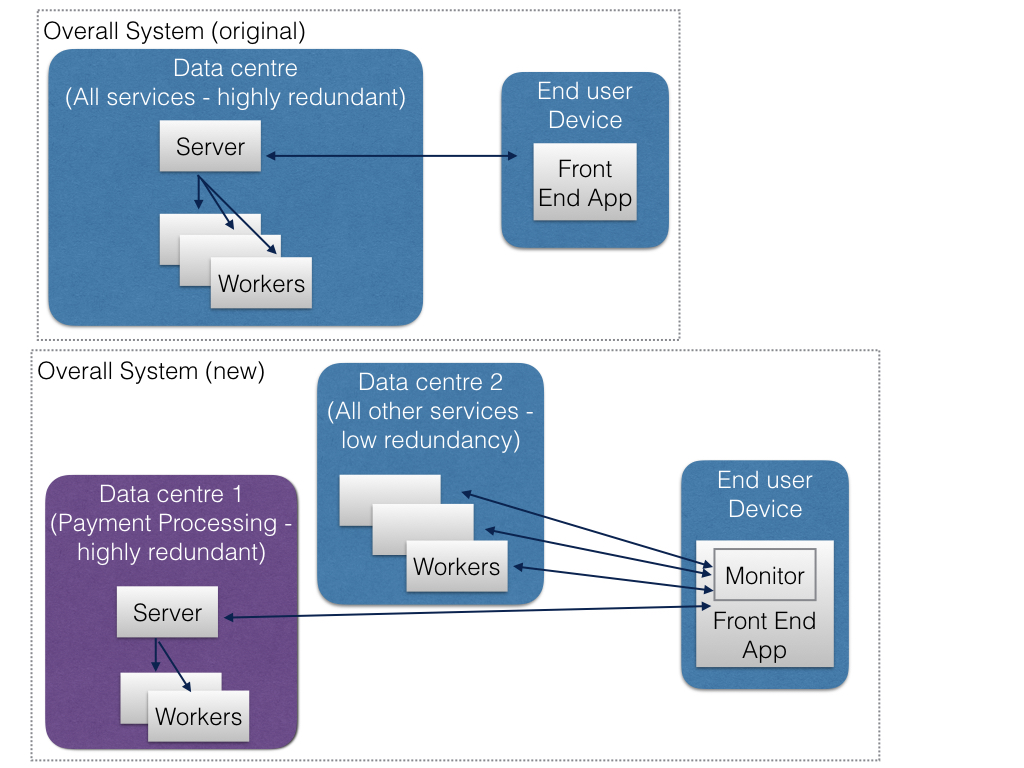
\includegraphics[width=\textwidth]{Figures/principles-styles}
\caption{eBay's Architectural Evolution for Energy Efficiency}
\label{figure:styles}
\end{figure}

This new architecture allowed eBay to achieve major capital and operational expenditure savings and well as reducing their energy consumption (and so "carbon footprint") significantly. This was due to the simpler design of the low-redundancy services, which have substantially decreased the amount and complexity of infrastructure needed.  As a consequence, they have achieved a significant reduction in datacenter build-out and fit-out costs and time scales. The underlying factor that allowed this improvement was that redundancy costs are significant. For example, according to Steven Shapiro, the cost of building a Tier III datacenter is double that of a Tier II datacenter \cite{shapiro2015-datacentre-mythsrealities}. (The Tier Classification System is a widely used rating system for datacenter availability, with Tier I being the least available or redundant facility and Tier IV the highest \cite{uptime2015-tierclassification}.)

Even more important (from our perspective), eBay has reduced energy consumption by approximately 50 percent because the low-redundancy site requires fewer infrastructure components (for example, N + 1 rather than 2N + 1 redundancy). This has resulted in  significant energy cost savings and also a reduction in maintenance and hardware refresh requirements, further lowering environmental costs.

\section{Conclusion}

There has been increased interest in reducing the significant energy costs of running large IT systems. However, little attention has been given to addresing energy efficiency at an application level, which limits its potential impact and prevents software architects from considering energy as a first class architectural concern.  When software architects do attempt to understand the energy property implications of their decisions, they find that they lack suitable tools and methods to address energy concerns when designing systems. With this challenge in mind, we've investigated how a large organisation solved this challenge and from that experience suggested three practical principles to guide architectural decision making, which architects can use to guide energy-related tradeoffs during system design even with today's limited knowledge and technology.

Despite these principles' simplicity, the eBay experience shows that they can yield significant cost and energy savings when applied to large-scale production systems. Savings of this scale are difficult to achieve through local optimizations, so we must address the problem at a system level, and ensure we allow software architects to work across stakeholder groups and organisational boundaries in order to achieve meaningful results.
 %Ch5 - Design Principles for Energy Efficient Applications

\chapter{Monitoring Application Energy Usage During Operation}

% Explain the problem we're trying to solve and the model for allocating it.


\section{Introduction}

The energy usage of information and communications technology (ICT) systems is starting to receive much more attention that it has historically.  This is due to the sharply increasing demand for electricity to run the digital economy, with US datacenters alone consuming an estimated 91 billion kWh in 2013 and are expected to consume 140 billion kWh by 2020 \cite{delforge2014-datacentreenergy}.

Researchers have been working for some years to understand the energy demand of ICT systems and significant progress has been made in a number of areas.  At the macro level, understanding how data centres use power and reducing the amount of power required in the data centre environment [REF].  At the micro-level, there have been some promising steps in understanding how individual programs consume power, to the point where it is possible to quite accurately predict and compare the power consumption of different options for program implementation [REF].

The problem for the software engineering practitioner is that their interest sits between these two extremes as they need to understand the energy consumption at the overall application level rather than at the individual component level or at the data centre level where many applications are consolidated.

The modern trend towards microservice-based systems [REF] makes things more complicated for the practitioner.  While it was possible to see ways of using program energy estimation approaches with monolithic applications, this quickly becomes overwhelming with a microservice-based system, due to the number of possible pieces of the system that could be involved in processing a workload or request.

In this chapter, we present the design for a piece of technology that we have designed to address this problem by fairly allocating the energy usage of a host machine to the application elements running on it.  Using modern microservice and operating system technology including containers, tracing and resource monitoring, combined with energy statistics for a machine, we can provide the host operator and the software architect with reliable estimates of the energy allocation of a machine's total consumption required to process requests for an application running on it.  This allows cost estimation and the evaluation of architectural alternatives to minimise energy consumption.

\section{Motivation}

There are several reasons to seek a method of estimating energy usage by software applications, but two immediate motivating examples in our case are cost estimation and architectural evaluation.

Today, the energy consumption of an application is not taken into account when considering its cost to operate and so there is little motivation for the software architect to understand and minimize their application's energy footprint.  This prevents large possible reductions in energy usage and its associated resources of environmental impact and cost.

Even where the architect is interested in the energy usage of their application, no mainstream and practical approach for estimating the energy usage of software at the application level is available.  This means that for applications where a significant number of system elements are used to process a request, as in a microservices-based system, it theoretically possible to use program-level approaches to estimate the energy usage, but is complex enough that we do not believe that it is done in practice.  This means that architects cannot evaluate the energy usage qualities of different architectural options.

The specific advanced achieved by this piece of work is the design an approach to measuring resource usage for request processing in a distributed application in such a way that an energy model can be used to estimate the energy usage of specific requests made to the application.

The goal of this is to provide a practical approach for software architects to estimate the energy costs of their applications and to evaluate different architectural options in terms of their likely energy usage.

\section{Microservice-Based Systems}

The microservice architectural style [REF] is rapidly becoming a mainstream approach for building industrial software systems and it is systems build using this style that we are specifically interested in for this work.
A microservice-based system is made up of many small, encapsulated, network-connected services, rather than the more traditional approach of having a small number of large servers that aggregated many services (a so-called "monolith" [REF]).

For our purposes, the important characteristics of a microservice-based system are:

\begin{itemize}
\item The business logic in the system is implemented as a group of small, focused services, each performing one task, typically implementing a "bounded context" in Domain Driven Design terms [REF].
\item The services are as independent as possible and have well defined service interfaces and only interact through these interfaces.  Resources such as databases are owned by a specific service and are not accessed by other services (hence a microservice-based system will have many independent data stores rather than a single consolidated database used by many services).
\item Handling an incoming request for a system is likely to involve a set of cooperating services, with one handling the initial request and then calling other services in order to fulfil the request and provide a response.  Microservice-based systems often separate request-handling and domain services but we do not assume that this is necessarily the case.
\end{itemize}

Well designed microservice-based systems typically share other important characteristics [REF], such as independent build, test and deploy for each service, and interfaces defined using machine readable formats such as Swagger [REF] and RAML [REF] but these other characteristics are not significant in the context of this work, and so we do not assume that they are present.

\section{Estimating Energy Usage}

As we investigated the problem of how to provide software architects, and other interested parties like data centre operators, with estimates of application level energy usage we identified a number of possible approaches.  

\begin{itemize}
\item Other researchers have tried to create entirely \emph{model based approaches} (such as [REF]) which can allow relative energy usage between different architectural structures to be estimated, but sidestep the problem of calculating actual energy values and require significant amounts of effort to create the models for non-trivial applications.

\item Other research projects have attempted to estimate architectural characteristics through \emph{event based simulation} but creating event based simulation models is an unfamiliar process to many practitioners and again is significant amounts of effort for non-trivial systems.  It is also the case that existing research in this area has not yet investigated how to estimate energy consumption, but rather has focused on other architectural qualities such as performance.

\item At the \emph{micro-measurement level}, sophisticated approaches have been designed to estimate energy consumption for individual algorithms or programs [REF-JOLINAR] with a high degree of success.  However these approaches rely on a highly controlled execution environment for the code being measured and access to low-level hardware state metrics, such as processor frequency statistics, in order to deal with the complex power characteristics of modern computing hardware.  While these models and tools are undoubtedly useful in the right situation, they are not practical tools for measuring the energy usage of a large-scale modern distributed application.

\item We explored whether we could combine the \emph{micro-measurement} approaches with \emph{application-level resource usage estimation} and produce meaningful energy estimates for the application-level workload.  However we found that approaches like Jolinar are not effective unless the low-level hardware state metrics can be provided and this wasn't practical in large distributed execution environments such as those used by microservice-based systems.

\end{itemize}

Having considered these options and realised that each of them had severe practical limitations, we shifted our focus slightly and reconsidered the goal of the work.  The problem we aimed to solve was to provide software architects and other interested parties with information on how to improve the energy efficiency of their applications.  The solution we identified to this problem was to shift our  goal from precisely estimating the \emph{actual} energy usage of a distributed application to estimating the \emph{fair allocation} of energy consumption to the application.  This is a useful goal because it allows service providers (such as cloud or hosting operators or data centre operators) to fairly allocate the cost of energy consumed by their infrastructure and it allows software architects to understand the energy consumption implications of their design decisions in relative terms, even if not in absolute energy consumption terms.

Our approach assumes that the energy consumption of the execution platform that the application is executing on is available to the energy calculation process and uses this, along with the total resource usage consumption of the execution platform and the resource usage of the application components to allocate the platform energy consumption to the different application elements running on it.  By tracing the execution of inbound requests across application elements, this allows us to allocate energy usage to specific requests and so compare the energy efficiency of different parts of a system and different design options for a system.

Estimating energy usage at the application level is a complex process and so it is important to be clear how the calculation will be performed before trying to design an implementation of it.

There are five quite distinct parts to the problem:

\begin{itemize}

\item \emph{Identification of service elements involved in processing a request}.  Processing a request in a modern distributed system will often involve a chain of service calls between the services that comprise the system logic.  We assume that the implementation of the services is under the control of those wishing to estimate energy consumption.

\item \emph{Identification of the processing periods attributable to a request}.  Once we know the system elements involved in processing a particular request, we need to identify when the element was performing work on behalf of the request.

\item \emph{Resource usage of the request}.  Given the system elements involved in processing a request and the periods when they were active, on behalf of the request, we need to estimate the runtime resources consumed by the system elements during these periods.  The resource consumption we need to estimate is the amount of CPU consumed, the amount of active memory in use, the number of network i/o bytes sent and received, and the number of disk i/o bytes read and written.

\item \emph{Estimation of resource and energy usage of the underlying host machine}.  Our aim is to fairly allocate the energy used by a machine during a time window across the requests that were active during that period.  Hence we need to estimate the overall resource usage of the machine and the energy that it consumed as a result.

\item \emph{Energy estimate of the request}.  Once we have the resource consumption metrics for a particular request, we then need to translate these into an estimate of the energy consumption that they imply.  We do this by establishing the percentage of overall machine resource utilisation that can be attributed to the request and then allocating the same percentage of energy usage of the underlying host to the request.

\end{itemize}

Each of these aspects of the problem has their own complexities, but they can largely be solved independently, and once resolved, it will be possible to achieve a reliable and fair energy allocation for each inbound request for a microservice-based system.  In the following sections of this chapter we discuss how each of these aspects of the problem can be implemented.

\section{Logical Design of an Energy Estimation System}

The functional design of a system to estimate energy usage for application requests (which we have dubbed "Apollo" - the Greek God of Prophesy, amongst other things [REF]) is shown in the informal block diagram in \ref{figure:logicaldesign}.

\begin{figure}
\centering
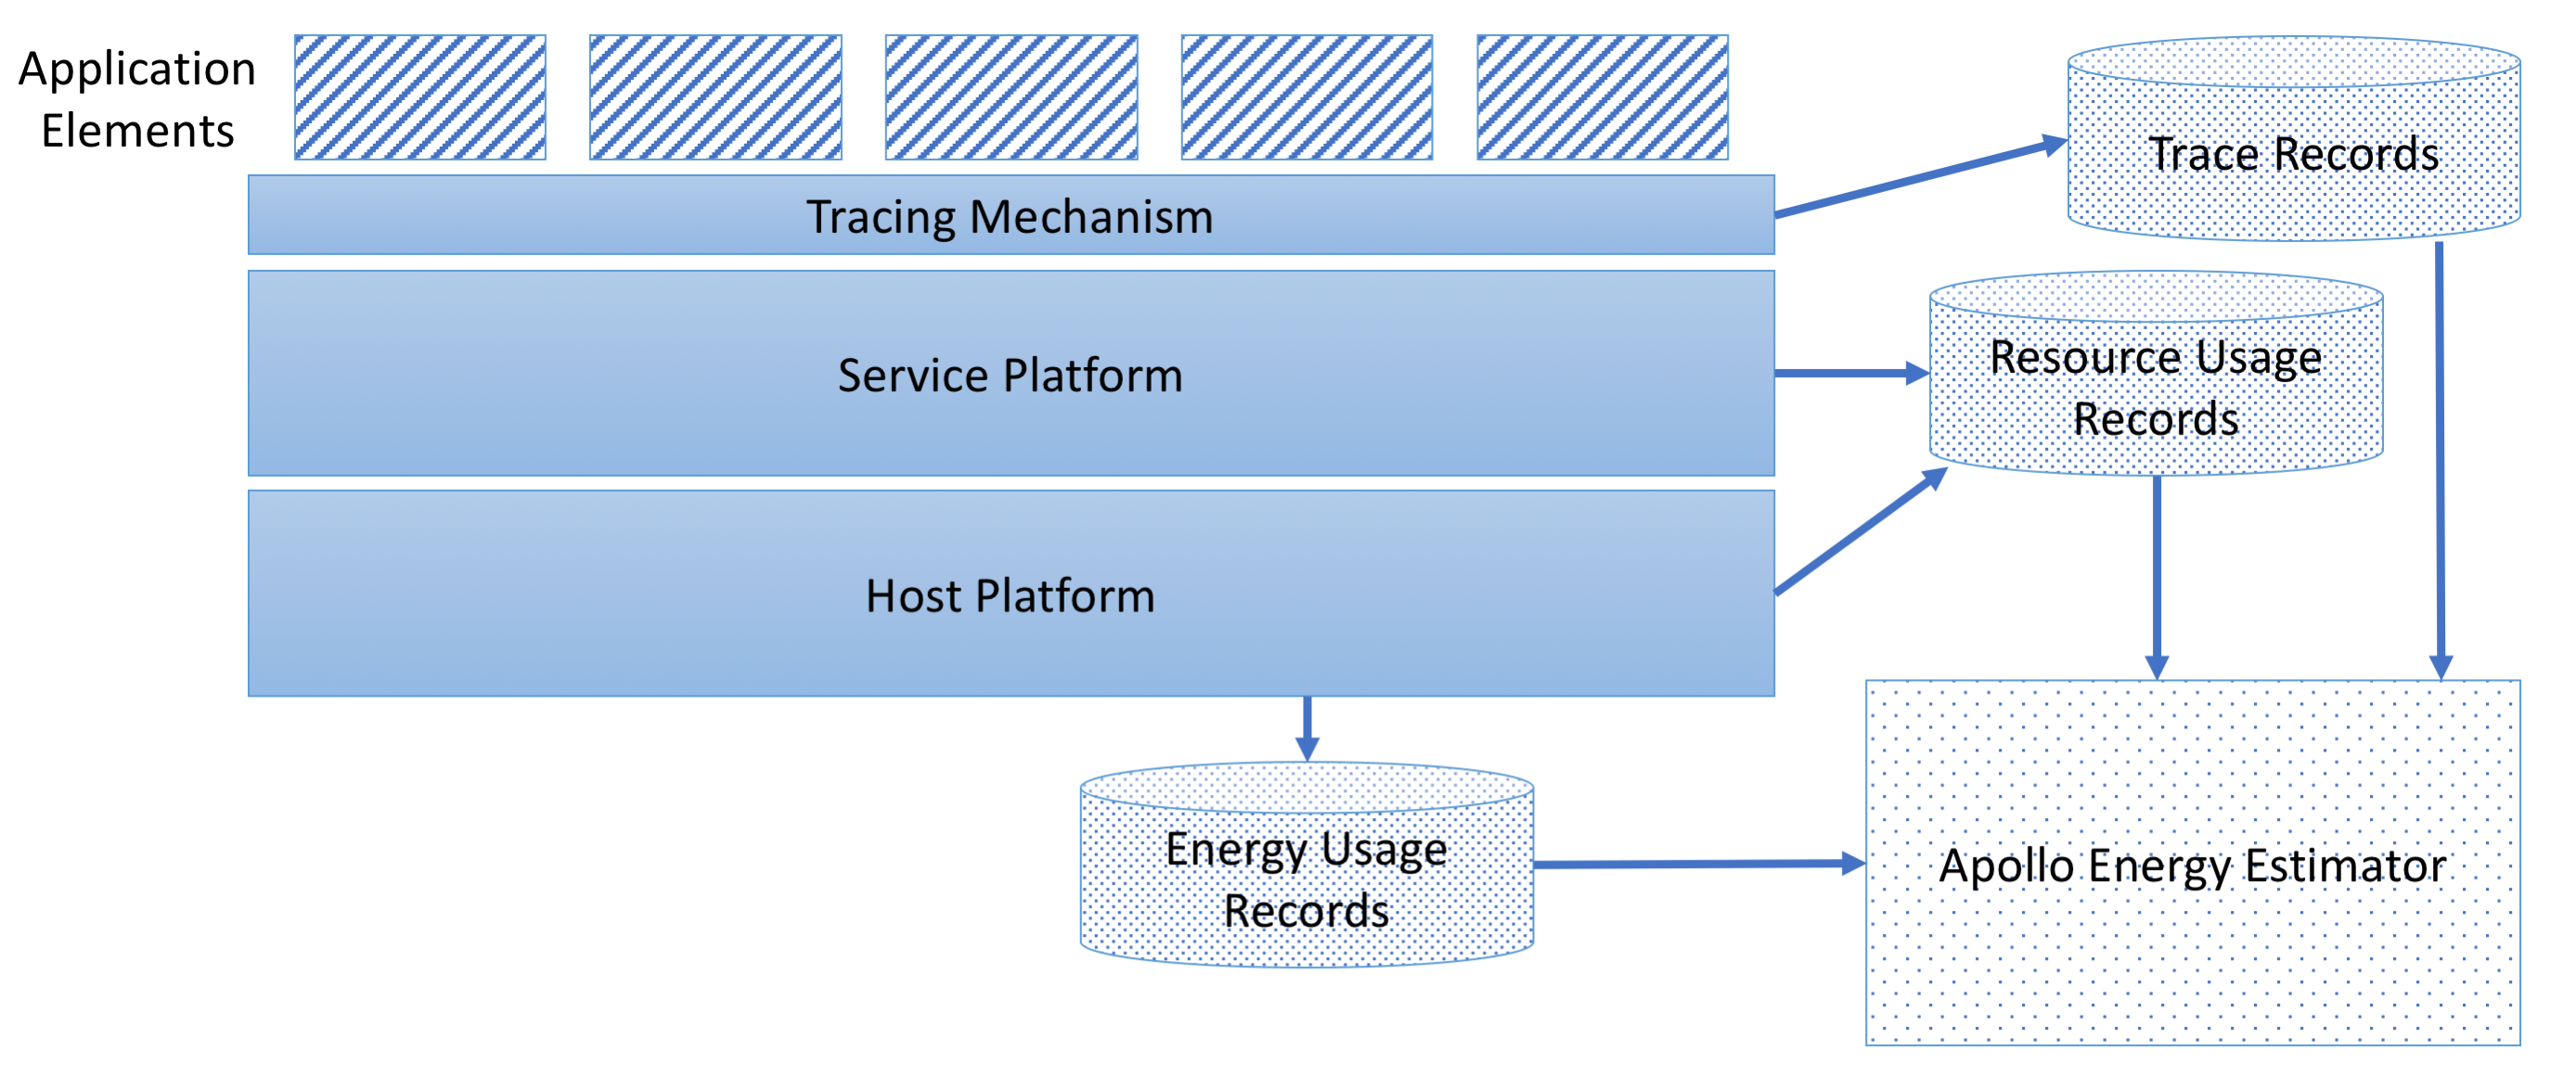
\includegraphics[width=\textwidth]{Figures/estimating-energy-logical}
\caption{Logical Design of the Energy Estimation System 'Apollo'}
\label{figure:logicaldesign}
\end{figure}

The elements in the diagram with solid fill are the underlying runtime platform and services, the diagonally hatched elements are the application under study, the densely-dotted elements are data, while the sparsely dotted elements are the Apollo energy estimation elements.

The elements of the system are briefly described below:

\begin{itemize}
\item \emph{Application Elements} are the architectural elements of the application which is being studied for energy consumption.  These are the main functional processing elements of the system, running in their own address space, providing a network interface to their services, invoked as part of request processing, with the implementation being under the control of the system owner who wants to estimate energy usage.  An example would be a request handling microservice to create an order.
\item \emph{Service Platform} is the system software which hosts the application components and can provide detailed measurements of their resource usage.  An example might be a PaaS platform like Cloud Foundry, a virtual machine or a container platform like Docker.
\item \emph{Host Platform} is the hardware and operating system platform that provides the general computing platform that hosts the service platform and provides runtime statistics on the platform's execution and energy consumption.
\item \emph{Tracing Mechanism} is key to our approach is the ability to trace which architectural elements were involved in handling a particular request for the system.  This tracing mechanism provides that ability, reporting the sequence of invocations of architectural elements and the time and duration of each.  Examples would be Zipkin and Jaeger.
\item \emph{Resource Usage Records} is a database of resource usage statistics for all of the functional elements of the system, fed from the Service Platform and the Host Platform.  An example could be Prometheus or InfluxDB, populated using a statistics collection server like Telegraf or cAdvisor.
\item \emph{Trace Records} is a database containing the request invocation traces from the Tracing Mechanism, which is likely to be a simple relational or document-oriented database, which the Tracing Mechanism writes its trace records to.
\item \emph{Apollo Energy Estimator} provides the key element of the energy estimation process, a calculator that works through the Trace Records and for each one, calculates which elements were active over which time periods, and uses the resource usage records to estimate the resource consumption of each request across the elements that were involved in processing the request.  These values are then compared with the overall host platform resource usage and the ratio of the values used to allocate the energy consumption of the host platform during the time period that the requests were active.

\end{itemize}

There are three key data structures in the design, which are critical to achieving the energy calculation, namely Trace Records, Resource Usage Records and Energy Usage Records.

\begin{itemize}

\item \emph{Trace Records} are created by the tracing mechanism and are used to record the invocation of system elements in processing a request.  There are two types of trace records, Traces and Spans.  Common features of the two are the identity of the runtime element writing the record, the start time of the record and the end time of the record.  A "trace" is written by the first element to handle an inbound request and its start time is when the request is received and its end time is when the response was dispatched.  A "span" records the activity of a single element in the handling of a request and it has a "parent" attribute which indicates the trace it is part of.  Should an element \emph{e1} cause another element \emph{e2} to be invoked, then the span recording the start and end times of the \emph{e2} activity has the \emph{e1} span as its parent.  Hence traces and spans are organized into a tree that mirrors the invocation structure of the request handling.  An example trace is shown in \ref{figure:span}.

\begin{figure}
\centering
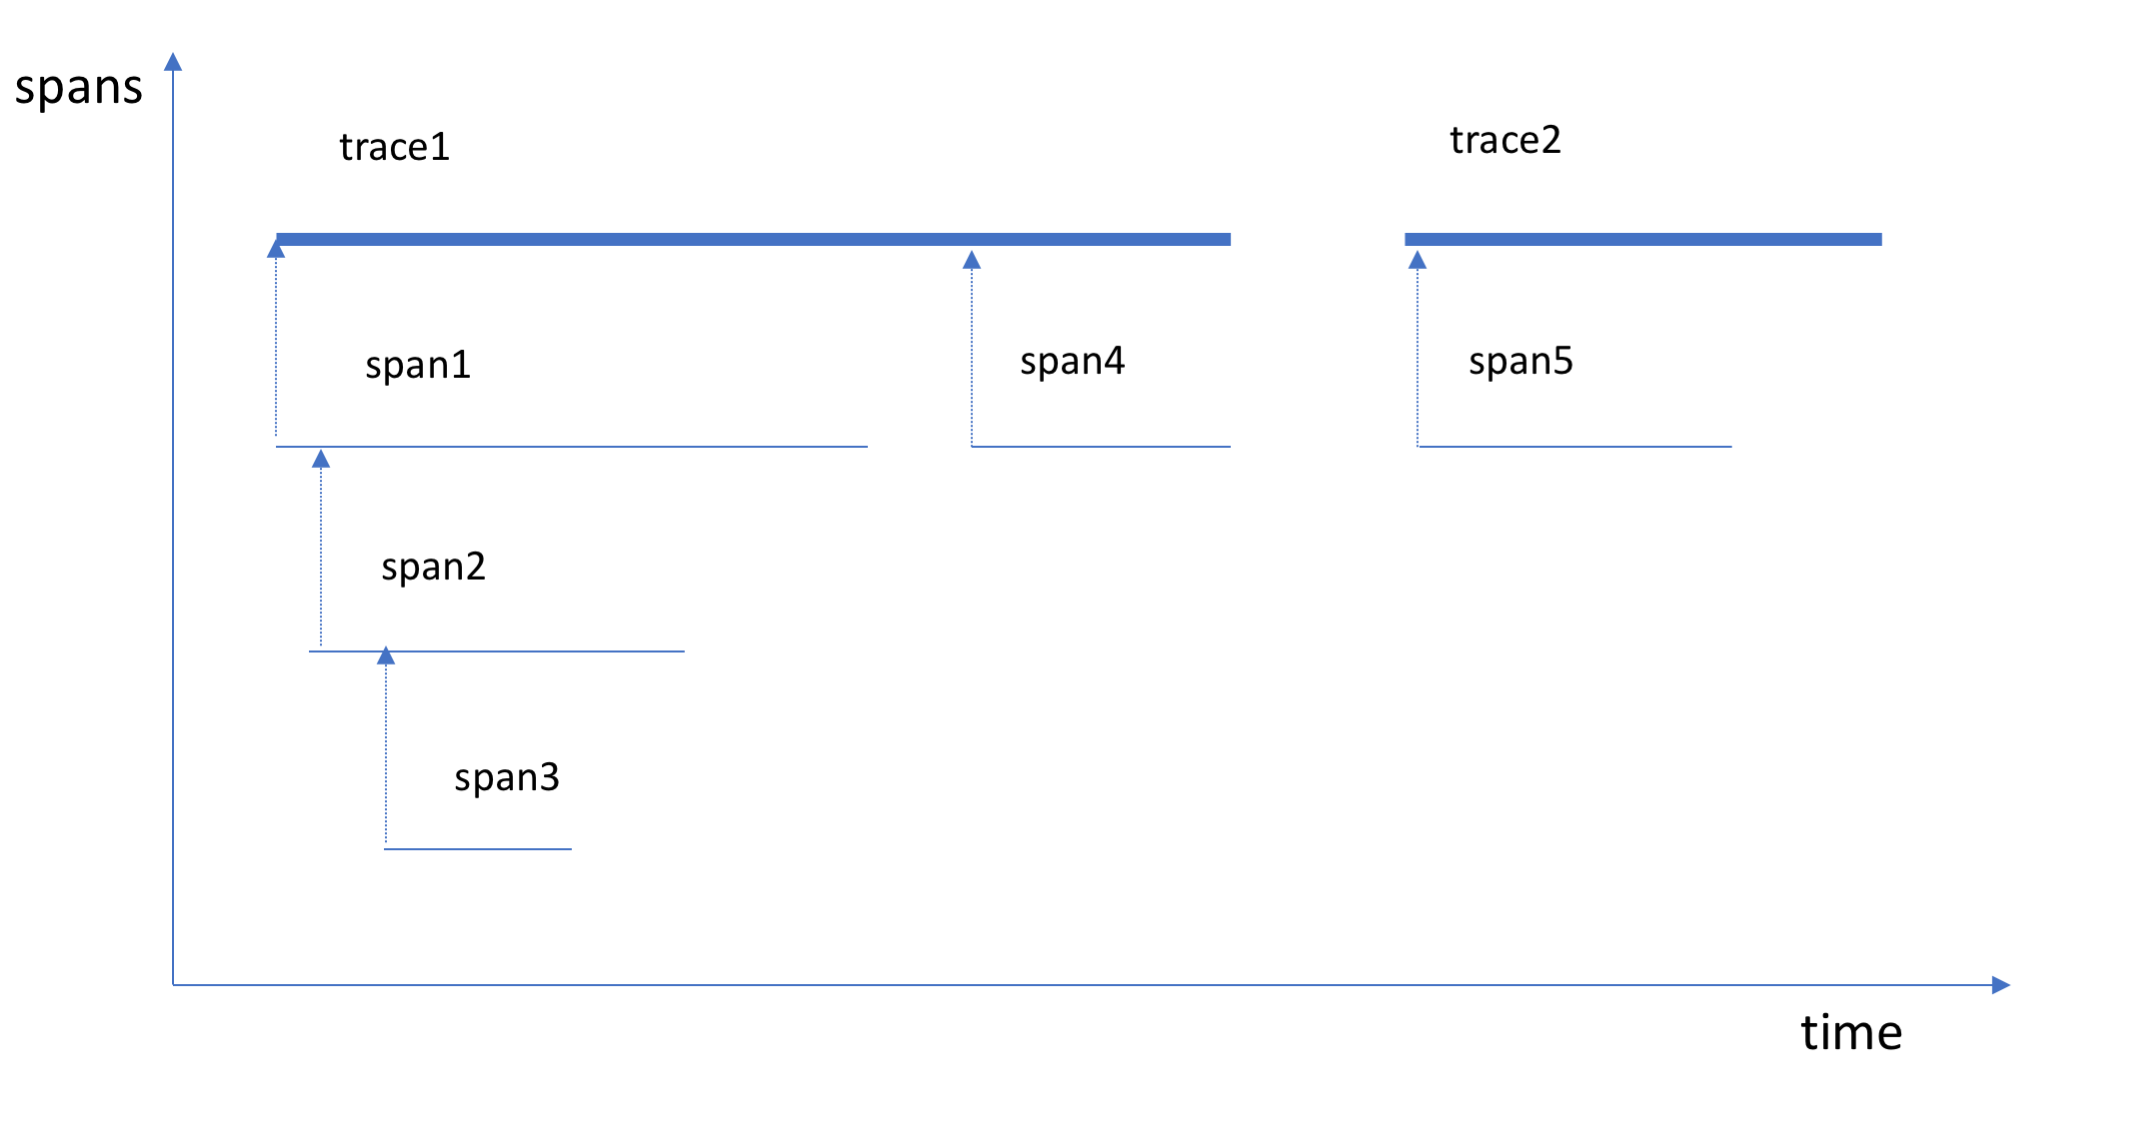
\includegraphics[width=0.75\textwidth]{Figures/estimating-energy-trace}
\caption{Example Execution Trace}
\label{figure:span}
\end{figure}

The figure shows two traces, representing requests, one after the other.  The traces are distinguished by not having parent spans, both traces have child spans, as indicated by the dotted arrows.  The y axis indicates invocation from top to bottom, the x axis indicates the passage of time.  The first request has two child spans, indicating that it invokes two other services.  Child span "span1" in turn invokes a third service, which invokes a fourth.  The second request invokes a single service.

\item \emph{Resource Usage Records} are generated by the runtime platform and stored in a timeseries style database to allow the metrics for a particular runtime element during a specified period to be retrieved (e.g. metrics for container c1 for the 3 second period from 20171105T084512.500 to 20171105T084515.500).  The metrics will be generated by the platform at regular but arbitrary intervals and so this data store will need to interpolate between the available measurement points to get the resource usage for the requested time periods.  The metrics that the runtime platform will be assumed to create are CPU usage (in "ticks" such as 1/100 second intervals), memory usage (in KB), disk IO (in KB) and network IO (in KB).  Absolute or cumulative measurements are both usable for our purposes.

\item \emph{Energy Usage Records} are ....

\end{itemize}

The key element in the system is clearly the Energy Estimator, which implements the fundamental algorithm to fulfil the purpose of the system.  This algorithm is sketched in pseudo-code below, with the architectural elements involved highlighted in bold text.

TODO











 %Ch6 - Monitoring Application Energy Usage During Operation

\chapter{Implementation of Application Energy Monitoring}
\label{chapter:implementation}

\section{Introduction}
The logical design of the Apollo energy estimation calculator was presented in Chapter \ref{chapter:monitoring} and showed how, in principle, we can build a useful energy calculator to fairly allocate energy usage of a collection of host machines, on the basis of the individual application requests processed in a period of time (rather than just the total resource usage of application elements over a period).   Such a calculator can provide a tool for a software architect to understand the energy consumption implications of their architectural decisions and can guide them towards higher energy efficiency for the applications.

The logical design of the calculator is independent of specific technologies and does not specify the details of the implementation, simply the operations that must be performed.  Hence, as we are now to implement the calculator, the logical design acts as our specification.  Our proof of concept implementation - Apollo - can be implemented in a number of ways using a number of different technology choices and detailed design decisions.

In this chapter we explain how we went about the task of implementing our proof-of-concept calculator, the problems we set out to solve, the choices we made, some of the problems we had to solve and some of the tradeoffs that were necessary.

\section{Defining the Context}

In order to focus our attention we needed to narrow the possible design space for our problem to allow us to focus on the key decisions specific to our research rather and avoid being distracted by the generic decisions that all software projects need to make.

These basic context-setting decisions were as follows:

\begin{itemize}
	\item As mentioned in the previous chapter, We will focus on the domain of \emph{microservice-based information systems}, such as those found in large enterprises, Internet-facing systems and Internet-oriented startup companies.  We will not specifically exclude the approach being used with other architectural styles, but where a design decision is required, we will assume that the approach will be used with a microservice-based system.
	\item We will assume that the primary technology "stack" used to implement the system will be \emph{enterprise Java}, meaning software written in Java, running on the JVM, using common open source frameworks and libraries like Spring Boot, Hibernate, Dropwizard, Spring Data, Apache Commons and so on.
	\item We will assume that the primary \emph{execution platform is Linux on Intel}, as this is something of a defacto standard for running large-scale enterprise Java systems.  Where it is possible we will try to make the approach execution platform agnostic (in particular to allow for Windows, another common server execution platform in the enterprise) but again, where a decision needs to be made, we will assume a Linux on Intel host.
\end{itemize}

All of these decisions align us with mainstream industry practice and provide practical options for applying our approach to industrial systems, while narrowing our design decisions to those related to our research problem, rather than generic concerns.

We discuss each of the more specific design problems we needed to solve and the decisions we made to solve each one in the following sections of this chapter.

\section{Tracing Application Execution}

Our aim is to provide the application architect with insight into the energy consumption implications of their design decisions, and so simply measuring the energy of the infrastructure hosting the application does not provide enough information for this purpose.  The architect needs to understand the energy implications of the execution of different parts of their application, and most importantly, the energy consumption of certain types of workload.  This will allow them to understand the energy intensive parts of their application and workload and focus on improving the energy characteristics of these application elements.  Comparing the energy characteristics of different elements and workloads will also allow them to see the implications of particular design choices.

This requirement means that we need some way of tracing the execution of workload through the application to produce data equivalent to the traces and spans that we saw in Chapter \ref{chapter:monitoring}.  We considered a number of ways of achieving this.

\emph{Application specific tracing} could be provided by an application as part of its implementation and write special purpose log files or database entries to record how an application request is processed through the application's elements.  While straightforward from our perspective, this is a complex and potentially time consuming feature to add to an application and would be quite complicated to add to an existing system.  We think that this approach would be unlikely to be adopted in practice.

\emph{Application Performance Management} (APM) tools, such as AppDynamics, New Relic and Dynatrace \cite{appdynamics2018, newrelic2018, dynatrace2018} already perform application request tracing to allow them to measure and estimate application performance characteristics.  Initially using a tool like this as the basis of our approach was our preferred option.  In practice though, while attractive to practitioners who were already using the particular tool we would choose, it is a significant barrier to everyone else due to the cost and complexity of deploying these tools.  While we see our work as a potential extension of APM tools, perhaps providing them with a new dimension to their facilities, we decided against basing our approach on one of them.

\emph{Microservice tracing systems} like the open source Zipkin and Jaeger \cite{zipkin2018, jaeger2018} projects were a third alternative that we considered.  These systems are used by application developers to provide standardised trace data about the execution of their applications and provide collection and analysis infrastructure to allow the trace data to be easily used.  When we initially investigated them, they appeared to solve part of the problem of implementing application specific tracing, but still left the application developer with significant work to do.  As we investigated these open source products further we found that they are supported by or integrated into many commonly used application frameworks (for example Zipkin is already integrated into libraries for about 10 languages, including Java, Python, C\# and JavaScript, and just considering Java, it is integrated into more than 15 well known application frameworks including Spring Boot, Dropwizard, Google RPC, Apache HTTP Client and Jersey).  If using a pre-integrated framework, using these tracing systems is very straightforward from an application developer's perspective and normally simply involves starting the data server to receive the trace data and setting some configuration parameters in the framework configuration.

After some experimentation we found that the Zipkin tracing system worked very well for a set of Java microservices and its database was easy to query to extract the trace information we needed.  We concluded that the reliability, easy availability, low implementation overhead, ease of use and large number of existing integrations with widely used application frameworks made Zipkin a good choice for our work.

\section{Estimating Resource Usage of Application Workload}

Once we can reliably trace execution of application requests through the application elements involved in processing them, we can move to considering how to estimate the resource usage of those application elements in order to work out the resource consumption of the requests processed by the application.  The key requirement here is to be able to collect reliable samples of the resource usage of the application elements on a very frequent and predictable basis (e.g. every couple of seconds).  Ideally the samples will be in terms of cumulative usage rather than usage at that point in time, as these are much easier to use for our purposes.

The only practical source of application resource usage statistics is the application execution platform.  There are a number of sources of statistics that we could use, each with slightly different characteristics.

The simplest option is to use \emph{native operating system tools} such as \texttt{sar} and \texttt{pidstat} on Linux and \texttt{procmon} and \texttt{perfmon} on Windows.  In principle these tools can collect resource usage statistics for application processes on the machine.  However in practice, our industrial experience and recent investigation for this work, suggests that they are really intended for collecting host-level statistics or for interactive investigation of a performance problem on a machine, by a skilled administrator.  They do not provide an easy way to get a reliable stream of samples of cumulative usage over time written into an accessible form.

An alternative is to bypass the tools and access the \emph{operating system performance counters} directly.  Like most modern operating systems, Windows and Linux both implement a set of performance counters in their kernels, which are used for monitoring performance and throughput of workload executed by the machine.  These counters are used by the operating system tools to provide the data they need to operate and so by accessing the counters directly, we can avoid any limitations in the tools and still achieve consistent results.  Linux provides access to its performance counters via the very convenient \texttt{{/proc}} file system, which exposes all of the kernel's counters for global and process-specific metrics, via a pseudo file system interface (which can be read using standard text processing tools or through the standard file system API).  Windows provides access to its performance counters via the \texttt{perfmon} tool or through an API which is accessible via PowerShell (the modern Windows scripting language) or a conventional programming language.  In principle we can build any collection tool we want using these interfaces or we can use metrics collection servers such as \texttt{telegraf} or \texttt{collectd} \cite{telegraf2018, collectd2018} to read them automatically and store them in a suitable database for us.  During initial research, this approach was our preferred option, however in practice we found it quite difficult to get a usable set of statistics for our application.  The main problem we faced was that the collector does not know which workload on the machine belongs to a particular application.  Therefore we had to collect everything at operating system process level, which potentially generates huge amounts of unnecessary data.  We also found that the business of building a reliable collector was more difficult than initially assumed and that linking the trace data to the dataset we could collect easily from operating system counters was quite difficult to do reliably.  These difficulties were not insurmountable, but led us to consider whether there were other options we could consider.

The third option we investigated was to use \emph{Docker} \cite{docker2018} as a packaging technology for the application elements and to allow us to collect resource usage statistics.  Docker is an operating system virtualisation technology which uses operating system mechanisms (such as "cgroups" and "kernel namespaces" on Linux) to isolate processes from each other, providing the illusion that each is running on a separate machine.  Docker also provides a packaging convention that allows software to be packaged into reusable packages called "images" which are combined at runtime to form runtime environment known as a "container".  Docker also provides a set of management APIs and tools to allow containers to be interrogated, managed and controlled.  Docker is rapidly becoming a de-facto standard in the industry to package, deploy and manage microservices both on general host computers (where Docker becomes an execution environment on top of the operating system) and more abstract, container based platforms like Kubernetes \cite{kubernetes2018} where Docker forms part of a sophisticated platform providing demanding quality properties like scalability and resilience, across a cluster of host computers.

Our interest in Docker lies in its ability to provide a low-overhead, isolated environment for running application elements (in our case, microservices specifically).  If we can assume that all of the microservices within our system are packaged and then run as Docker containers then it provides us with the ability to extract accurage resource utilisation statistics for the microservice running in the container.  Another benefit of using Docker is that each container has its own network (IP) address which can be found via the runtime metadata available via Docker's management API.  This greatly simplifies the process of relating the resource usage data to the request traces from Zipkin as the network address is a shared piece of information between the two.

We believe that requiring application elements (the microservices) to be packaged and run as Docker containers is realistic and reasonable, given its wide and growing adoption in industry, particulary for microservice-based systems.  Therefore this combination of factors resulted in us deciding to use Docker as the basis for collecting application resource utilisation statistics.

A useful side effect of packaging the application as a set of microservices in containers is that it makes the utilisation of the trace data simpler.  The trace data identifies the application elements by network address (typically IP address and port number).  Each container in a Docker deployment (strictly a Docker network) has its own set of one or more IP addresses.  Therefore, by having each application element in a separate container, we can rely on them listening on different IP addresses and for the container to IP address mapping being available from the Docker meta data.  Hence this approach to application packaging and deployment makes the mapping of trace data to application elements straightforward. 

The second part of collecting utilisation statistics is how they are extracted and stored from the execution platform.  In our case, our experimentation with Docker quickly revealed that a number of open source projects, including \emph{cAdvisor} \cite{cadvisor2018} and \emph{Telegaf} \cite{telegraf2018}, provide close integration with Docker and can extract and store the utilisation statistics data in different database systems.

After some experimentation we chose to use Docker with Telegraf, storing utilisation statistics in the \emph{InfluxDB} \cite{influxdb2018} open source time-series database to provide us with reliable application element resource utilisation statistics gathering.

\section{Estimating Resource Usage of the Host Platform}

Estimating resource usage of the underlying host platform is simpler than gathering the same information for the application elements, as host-level statistics gathering is a mature and widely used technology, provided by all major operating system platforms.

In our case we need to achieve reliable resource utilisation sampling of the host platform - the underlying Linux operating system - and have them stored in a database that allows us to extract them through a query interface to support the calculation process.  Ideally if the statistics are in a similar form to the statistics for the application level resource utilisation (e.g. the same timestamp convention and data types used), then this is likely to make the implementation of the calculator easier.

Our earlier investigation of the \emph{Telegraf} data collection server to extract and store application-level utilisation statistics revealed that it can be configured to extract and store host-level utilisation statistics too, and that this facility is provided as part of the standard distribution of the (open source) product.  When we tested the host resource utilisation statistics feature of Telegraf we found that it was straightforward to use and reliably stored accurate statistics in the same database as the application-level statistics.  The host-level statistics used the same basic conventions as the application-level statistics (e.g. they were both cumulative utilisation statistics using the same timestamp conventions).

Therefore we were able to solve the host-level resource utilisation statistics gathering problem by simply extending the configuration of the Telegraf server and the extension of the data set it stored to include host-level statistics.

\section{Estimating Energy Usage of the Host Platform}

As explained when we discussed the motivation for this work in Chapter \ref{chapter:introduction} the field of energy estimation is relatively young and reliable approaches for energy estimation of individual devices and applications are only just emerging.  Our work does not intend to address the problem of estimating energy consumption for a single host computer, but rather requires a reliable energy consumption metric to be available.

As explained in Chapter \ref{chapter:monitoring} there are two main approaches available to us that can provide energy usage of our underlying host platform, physical energy consumption metrics made available via a DCIM platform and model-based energy consumption estimation using machine utilisation levels and published benchmark results.

In many industrial situations a DCIM platform will be available and energy consumption metrics for all or a significant subset of host machines will be available through it.  However in our research environment we did not have access to such a platform and in many industrial situations this will be the case too.  While the state-of-the-art in organisation design is to integrate development and operations groups, they are frequently still separate and so even when a DCIM platform is available, software architects may well not be able to access it easily.

Therefore we decided to use a model-based approach to estimate the energy consumption of the host, but to ensure that it was easily replaceable with alternative models or with queries to a DCIM platform if one was available.

The approach used to estimate the energy usage of a host was explained in section \ref{subsection:calculation-specification} and relies upon published power consumption benchmark results associated with the SPECpower\_ssj 2008 benchmarks \cite{lange2009-specpower}.  An example data set for power consumption for a specific model of server host is shown in \ref{table:powervalues}.

\begin{table}
\centering
\caption{SPECPower 2008 Benchmark Results for \\Dell PowerEdge R730 (Intel Xeon E5-2699 v4 2.20 GHz)}
\label{table:powervalues}
\footnotesize
\begin{tabular}{|c|c|c|}
\hline
Machine Load & Power Consumption (W) & W / \% \\
\hline
\hline
Active Idle  &  44.6 & -    \\
10\%         &  84.8 & 8.48 \\
20\%         & 102.0 & 5.10 \\
30\%         & 120.0 & 4.00 \\
40\%         & 136.0 & 3.40 \\
50\%         & 150.0 & 3.33 \\
60\%         & 163.0 & 2.64 \\
70\%         & 181.0 & 2.58 \\
80\%         & 205.0 & 2.56 \\
90\%         & 238.0 & 2.64 \\
100\%        & 272.0 & 2.72 \\
\hline
\end{tabular}
\end{table}

We use this style of benchmark data combined with the machine type executing our application workload and the utilisation level metrics of the server executing the load to estimate host server energy consumption at a particular point in time, as explained in section \ref{subsection:calculation-specification}.

The third column in the table is a derived value we have added to show the power consumption per percentage point of server utilisation at each level of utilisation.  This clearly illustrates the need to keep servers busy from an energy efficiency perspective as it can be seen clearly that 1\% utilisation when the machine is quiet is three times more expensive in energy consumption terms than 1\% utilisation when the machine is busy.  We investigate this observation further in Chapter \ref{chapter:validation} when we describe how we validated the implementation of Apollo.

\section{Implementing the Calculator}

\subsection{Design of the Calculator}

The design of the Apollo calculator is shown in the simple block diagram in Figure 3. The system element filled with the fine dotted pattern represents the architectural elements of the application (i.e. an application microservice), the system elements filled with the fine cross-hatching are data elements, while the Apollo Energy Estimator is filled with the light solid fill.  The unshaded elements are the third party technologies which are reused unchanged as part of the implementation.

\begin{figure}
\centering
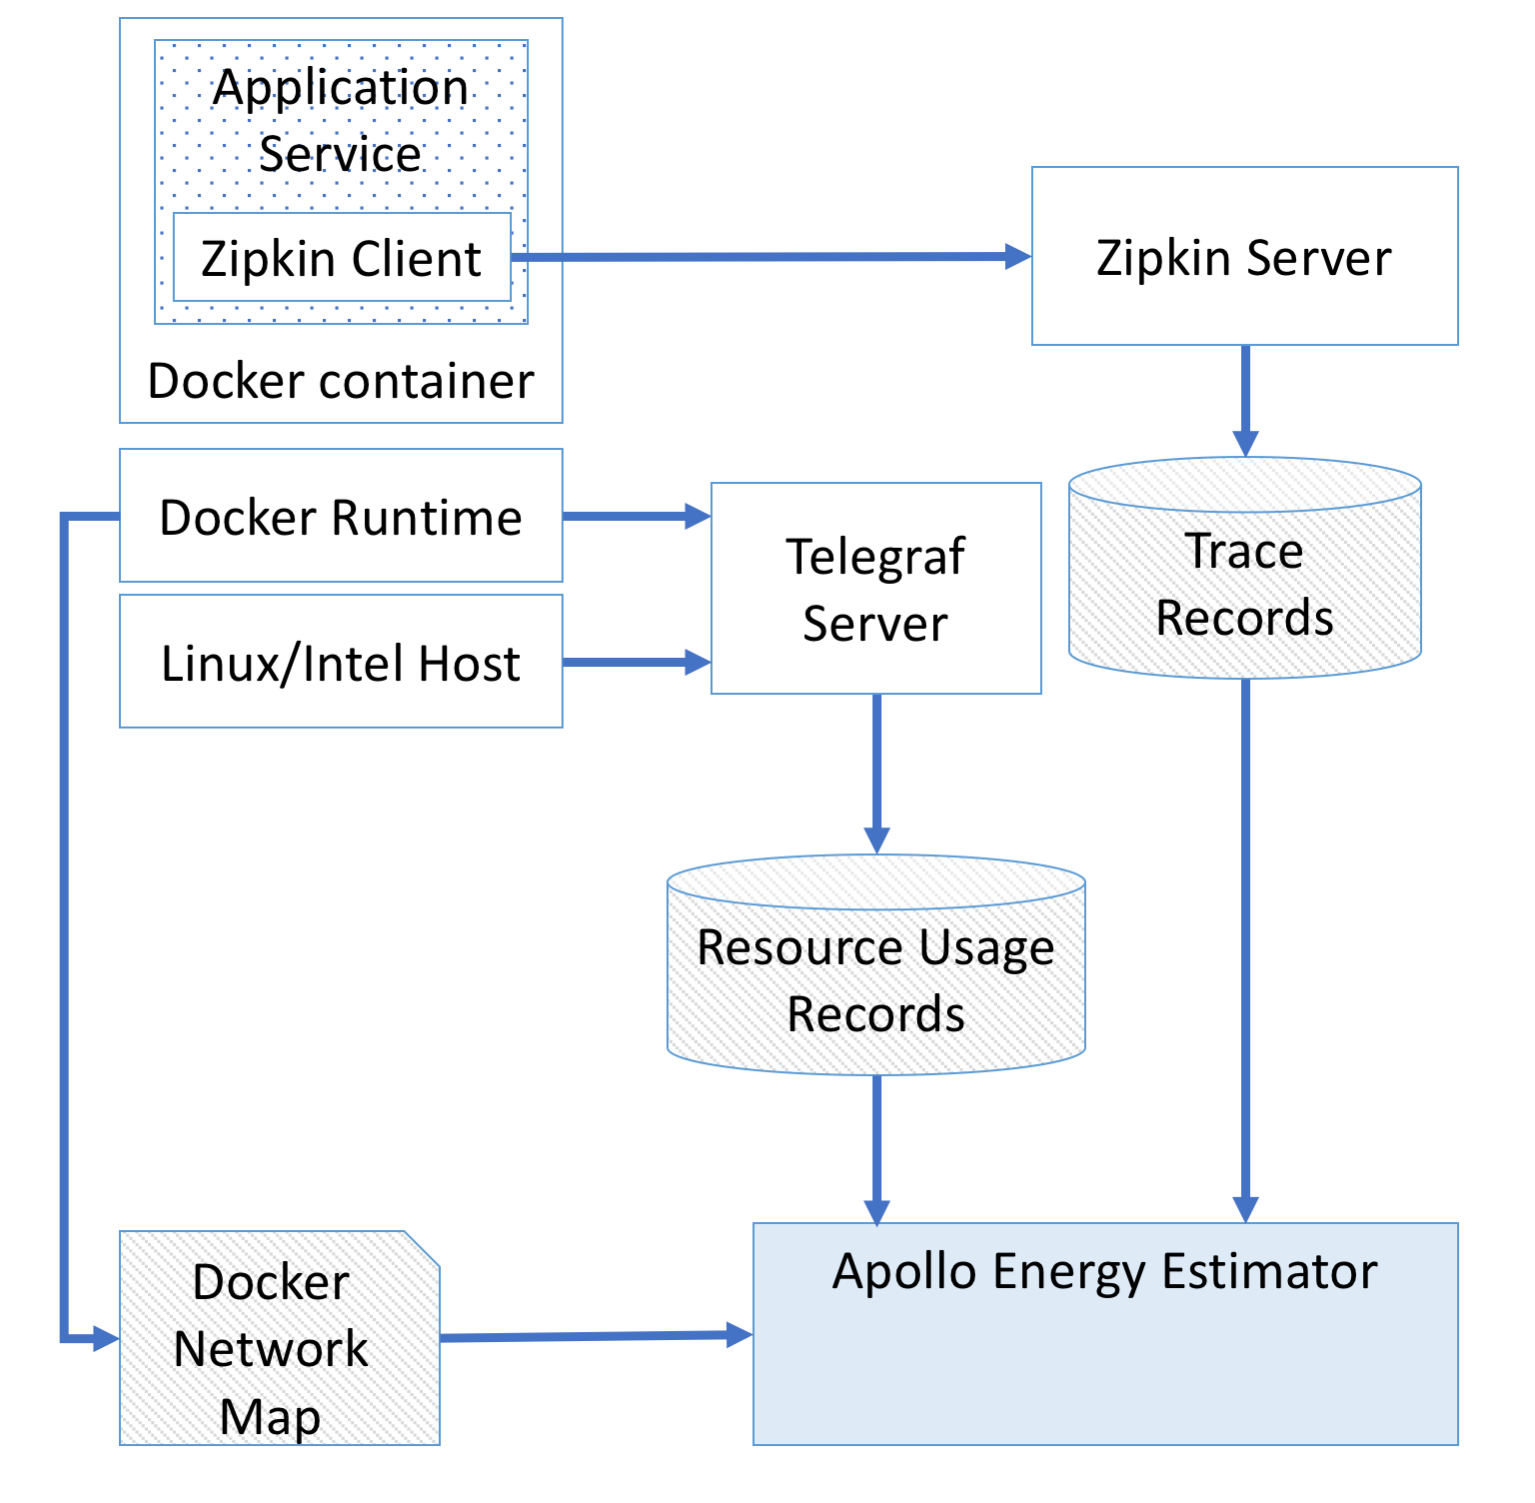
\includegraphics[width=0.5\textwidth]{Figures/implementation-design}
\caption{Design of the Apollo Energy Calculator}
\label{figure:implementation}
\end{figure}

The design elements of the calculator and their responsibilities are summarised in Table \ref{table:designelements}

\begin{table}
\centering
\caption{Apollo Energy Calculator Design Elements}
\label{table:designelements}
\footnotesize
\begin{tabular}{|l|p{10cm}|}
\hline
\textbf{Design Element} & \textbf{Responsibilities}  \\
\hline
\hline
Application Service & This element represents the regular microservices that comprise the application under investigation.  The implementation of these services are under the control of the development team and they have the responsibility to generate Zipkin trace records (via the Zipkin Client library) to record their activity (although this will usually be achieved automatically through use of an application framework like Spring Boot). \\
\hline
Zipkin Client & A trace of the invocations to and between application elements is required and as explained above, the Zipkin tracing system is used to achieve this.  The Ziplin Client is a client programming library used by Application Services to generate trace records and forward them to the Zipkin Server for storage.  The application code may invoke this library directly or it may be invoked automatically by an application framework like Spring Boot or Drop Wizard. \\
\hline
Zipkin Server & The Zipkin server receives and stores the trace records from the Application Services.  One Zipkin Server is used for all of the Application Services in a monitoring context. \\
\hline
Trace Records & The Zipkin Server persists the trace records in a well defined schema in a database.  In our case we used MySQL as the database for the trace records. \\
\hline
Docker Container    & All application elements need to run within Docker containers.  This allows metadata about the elements to be retrieved and resource usage statistics to be gathered.  This container contains the Application Service (each service is packaged in a separate container to allow it to be monitored separately).\\
\hline
Docker Runtime     & The Docker Runtime is part of the Docker system software package and provides the control and monitoring of the Docker containers in the application and provides runtime statistics for the containers, which in our situation are streamed to the Telegraf Server for storage. \\
\hline
Linux/Intel Host   & The application runs within Docker on the underlying host machine(s) and we have chosen to use an Intel host running the Linux operating system, due to the maturity of both Java and Docker on this platform. \\
\hline
Telegraf Server & The Docker platform produces a stream of resource usage statistics for the containers that it is executing.  The Telegraf open source metrics collection agent collects these metrics and stores them in a timeseries database for easy retrieval. \\
\hline
Resource Usage Records & The Telegraf Server generates a stream of resource utilisation statistics by constantly querying the Docker Runtime and the Linux Host.  These statistics records are persisted to a database for later use.  The datastore used for the Resource Usage Records is InfluxDB, an open source timeseries database. \\
\hline
Docker Network Map & The Zipkin traces and the resource usage records identify the runtime elements of the system in different ways; the Zipkin traces are collected at the network level and so identify elements by IP address and port number, while the Docker resource usage statistics are identified by Docker container ID.  Hence metadata is needed to link the two together and this is the purpose of the Docker Network Map which is metadata available from the Docker Runtime (through the \texttt{docker network inspect} command) which allows us to find the IP address(es) in use by each container during the execution of the application. \\
\hline
Apollo Energy Estimator & The Apollo module collects data and implements the energy allocation algorithm described in Chapter \ref{chapter:monitoring}.  This module is the primary software that we have implemented as part of this research (along with an example application we use for validation, which we describe in Chapter \ref{chapter:validation}). \\
\hline
\end{tabular}
\end{table}

Most of the system described here is open source software (Docker, Telegraf, Zipkin, InfluxDB, MySQL and Linux) and so the only significant piece of custom software that had to be developed for this investigation was the Apollo Energy Estimator module.  The other software development effort was configuration and scripting to combine the different pieces of software into a single system.  We describe the software design of the Estimator module in the next section.

\subsection{Data Design}

In the earlier subsections, we explained how we would solve each of the data gathering problems in order to create the data sets that the energy estimator requires in order to perform its calculations.  We now need to define how that data is used by the calculation code.

The data model for the data from the different sources is shown using the UML class diagram in Figure \ref{figure:data} and the data elements are described in Table \ref{table:dataelements}.

\begin{figure}
\centering
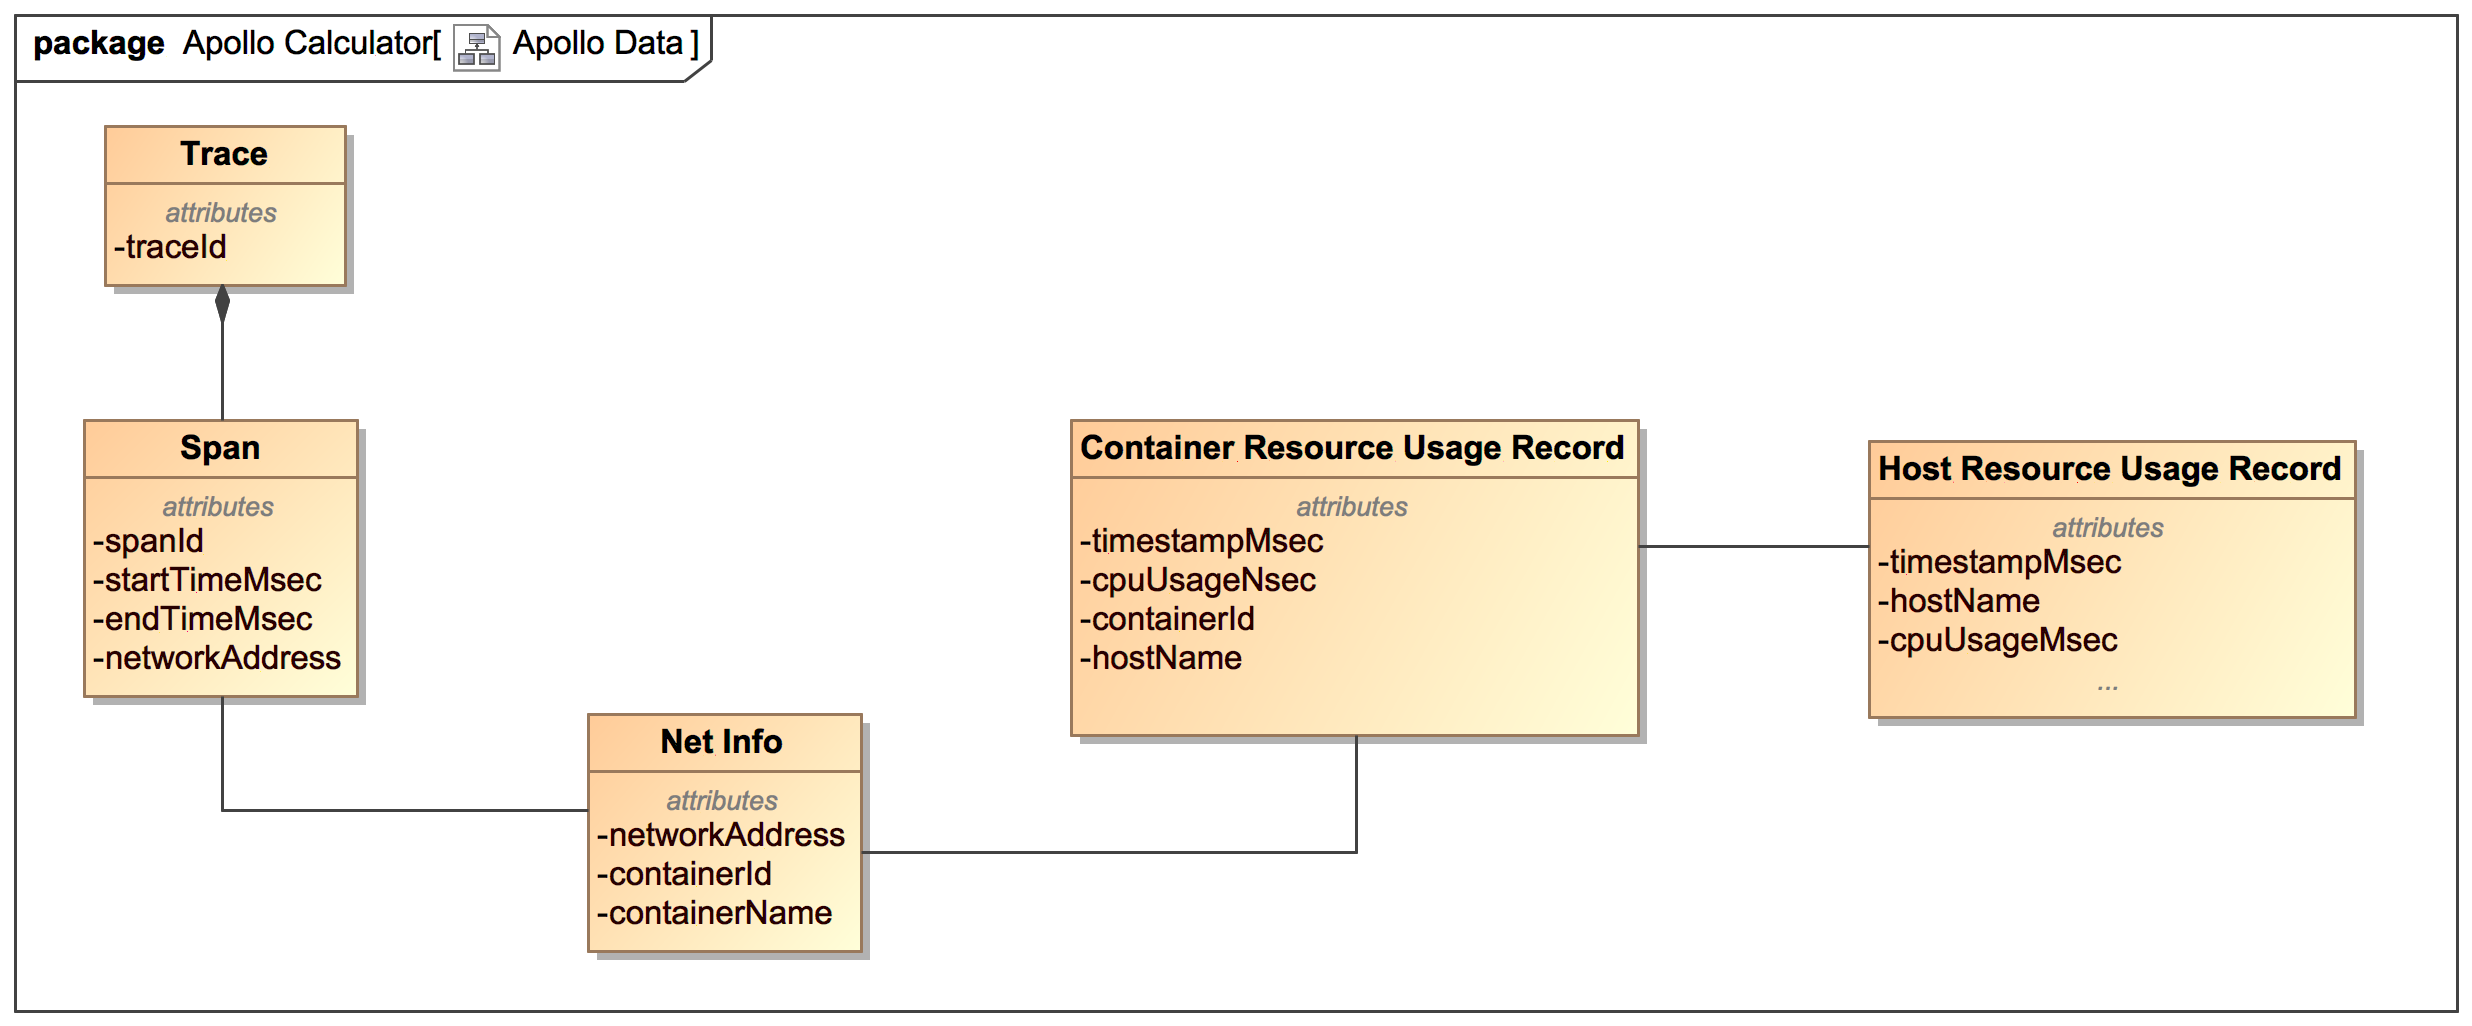
\includegraphics[width=1.0\textwidth]{Figures/implementation-data}
\caption{Data Structure for Apollo Energy Estimator}
\label{figure:data}
\end{figure}

\begin{table}
\centering
\caption{Apollo Energy Calculator Data Elements}
\label{table:dataelements}
\footnotesize
\begin{tabular}{|l|p{10cm}|}
\hline
\textbf{Data Element} & \textbf{Description}  \\
\hline
\hline
Trace & The \textit{Trace} is just a simple container for a set of \textit{Spans}.  While the Zipkin data item does contain more information, from our perspective, we are only interested in it having a unique ID.  This is sourced from the Zipkin data set.\\
\hline
Span & Contains the information recording a specific invocation of an application element.  One \textit{Span} is written for each application element invoked as part of a trace.  Identifies the application element by \textit{networkAddress} (an IP address in our case) and records the start and end time of the invocation in milliseconds.  Composed into exactly one \textit{Trace} and so contains its ID to record the relationship.  This is sourced from the Zipkin data set. \\
\hline
Net Info & Provides a mapping between network addresses, (Docker) container IDs and container names.  Any network address maps to exactly one container ID and one container name.  This is sourced from the Docker Network Map data set. \\
\hline
Container Resource Usage Record & Records the resource usage of a specific container at a point in time.  Contains the sample time as a millisecond timestamp, the cumulative CPU usage in nano-seconds measured at that point, the ID of the container being measured and the hostname of the computer it was executing on. This is sourced from the Docker resource utilisation statistics collected by Telegraf (and stored in InfluxDB).\\
\hline
Host Resource Usage Record & Records the resource usage of a host computer at a point in time.  Contains the sample time as a millisecond timestamp, the cumulative CPU usage in milliseconds measured at that point and the hostname of the machine.  This is sourced from the operating system resource utilisation statistics collected by Telegraf (and stored in InfluxDB). \\
\hline
\end{tabular}
\end{table}

The basic data access path required is to start with the \emph{Trace} and iterate over the \emph{Spans} that it contains.  For each span, use the \emph{startTimeMsec} and \emph{endTimeMsec} to establish how long the invocation was for and when it was.  Using the \emph{networkAddress}, the \emph{containerId} can be identified using the \emph{Net Info} data.  This allows the resource usage records for the container to be identified using the start and end time and the container ID.  Then, to establish the resource utilisation of the host during the same period, the \emph{hostName} attribute of the \emph{Container Resource Usage Record} and the start and end times can be used to identify the correct \emph{Host Resource Usage Records} to use.

Therefore, as can be seen, this data stucture allows us to navigate through the data sets to find container and host resource utilisation data for each of the spans in a trace.

There is one remaining problem however, which is the fact that the spans are periods of time, but the usage records are samples at a point in time.  We need to solve this problem to use the data correctly.

In our specification, in Section \ref{subsection:calculation-specification} we could assume an ideal, technology independent, situation where it was possible to use simple interpolation to estimate the CPU usage between two points, however close or far away they are.  This of course relies on very frequent sampling so that any error caused by averaging between the start and end of the sample does not distort the result in a material way.

As we investigated the technologies that could provide resource utilisation metrics, we discovered that sample intervals for real resource utilisation statistics, such as those provided by operating systems or Docker, are actually very long when compared to request durations.  A typical sample interval for Docker is 10 seconds and an operating system might be 1 minute, whereas a request duration may only be 10s of milliseconds.  Sample intervals can be reduced in duration (at the cost of monitoring overhead and data volume) but realistically they can only be reduced to 5 - 10 seconds, not the durations that match request durations.

\begin{center}
\fbox{
\parbox{0.75\textwidth} {
\textbf{TODO} - fundamental decision here ... do I rework the spec or continue this argument?   On balance reworking the spec seems better as it makes the spec (slightly) simpler and makes this chapter much easier to write.  But it does bring in limitations at the spec level.
}
}
\end{center}





\subsection{Software Design and Implementation}

The Apollo estimator does two primary things, it gathers data from the resource utilisation statistics, the trace records and the Docker network meta data and it uses the information to perform the energy allocation processing required to establish the energy characteristics of each of the inbound requests to the application, described in the trace records. 

The implementation of the module is described by the UML class diagram in Figure \ref{figure:classes} and the class descriptions in Table \ref{table:classes}.

\begin{figure}
\centering
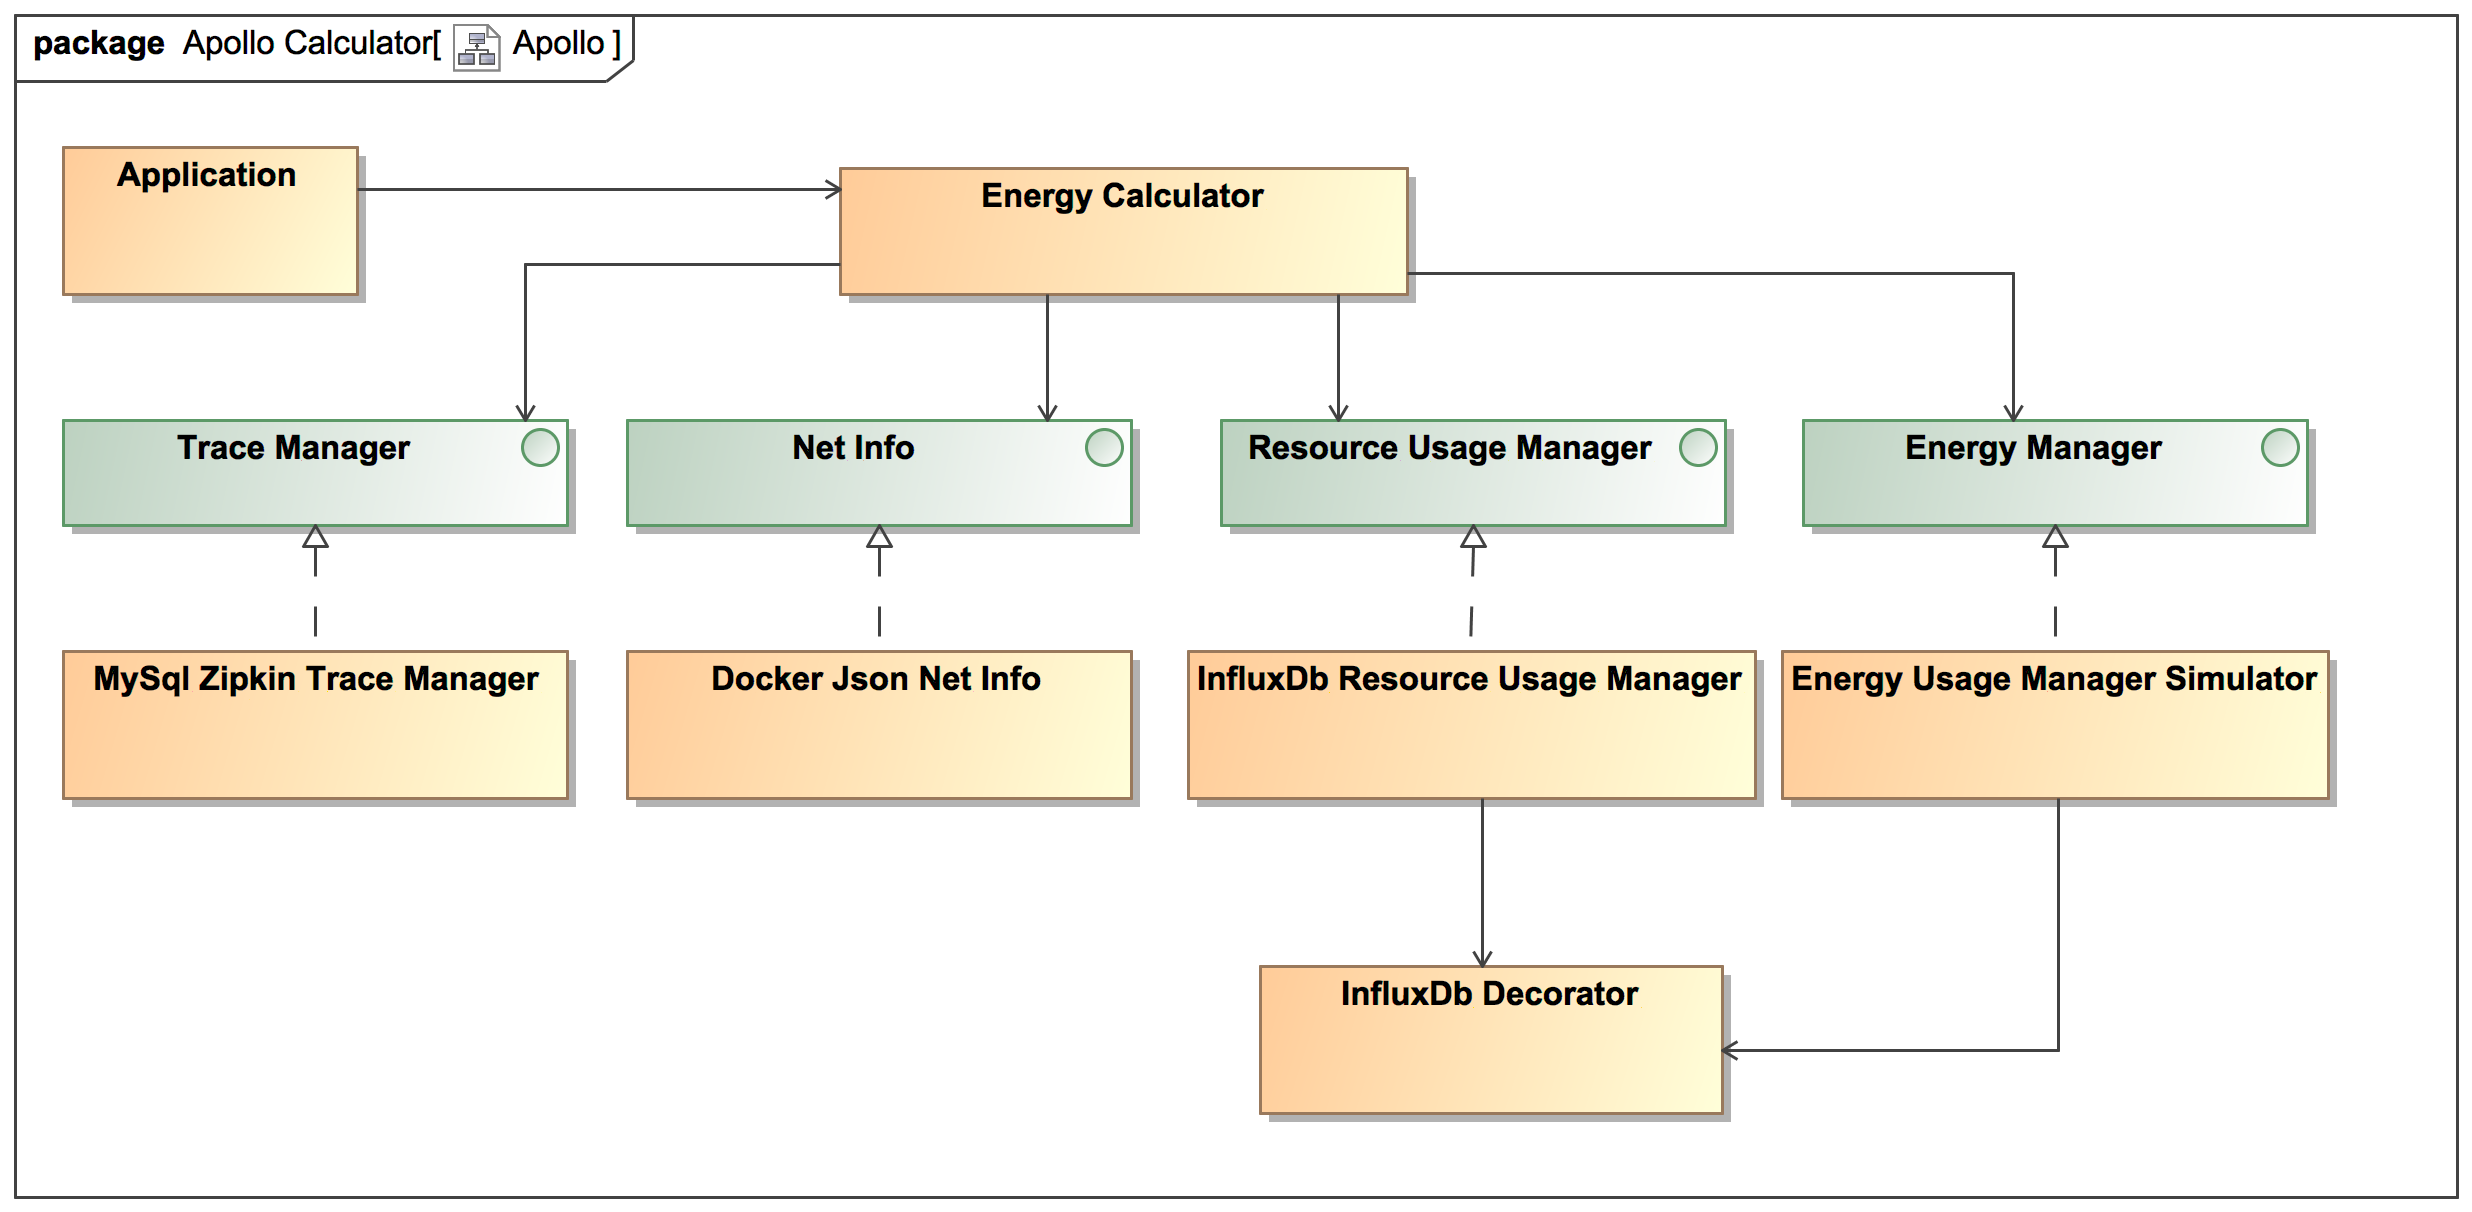
\includegraphics[width=1.0\textwidth]{Figures/implementation-classes}
\caption{Implementation of the Apollo Energy Estimator Module}
\label{figure:classes}
\end{figure}

\begin{table}
\centering
\caption{Apollo Energy Estimator Module Structure}
\label{table:classes}
\footnotesize
\begin{tabular}{|l|p{10cm}|}
\hline
\textbf{Design Element} & \textbf{Description} \\
\hline
\hline
Application & This is a small "bootstrap" class with the responsibility of loading configuration settings, creating the other elements and providing an entry point for the runtime system. \\
\hline
Energy Calculator & Provides the main processing loop to retrieve traces from the \texttt{Trace Manager}, retrieve the corresponding data for each trace from the other elements and then perform the required calculation. \\
\hline
Trace Manager & An interface defining a simple API to retrieve trace records. \\
\hline
MySql Zipkin Trace Manager & An implementation of the \texttt{Trace Manager} interface that accesses the Zipkin Server's MySQL database to retrieve the trace records held within it. \\
\hline
Net Info & An interface defining a simple API to allow container IDs to be mapped to network addresses and vice versa and container names to be mapped to container IDs and vice versa. \\
\hline
Docker Json Net Info & An implementation of \texttt{Net Info} to provide the container name, ID and network address mappings from the JSON file produced by the Docker \texttt{docker network inspect} command. \\
\hline
Resource Usage Manager & An interface describing the API to retrieve resource usage information during a period of time for a Docker container, for a host machine or for a host machine where a specific container ran. \\
\hline
InfluxDb Resource Usage Manager & An implementation of \texttt{Resource Usage Manager} that retrieves the information from an InfluxDB that has been populated by the \texttt{Telegraf} metrics capture server. \\
\hline
Energy Usage Manager & An interface defining the API that provides the ability to retrieve energy usage information for a host machine by name for a period of time, or a host machine that a particular container ran on during a period of time. \\
\hline
Energy Usage Manager Simulator & An implementation of the \texttt{Energy Usage Manager} interface that uses a simulation based approach to provide realistic energy consumption information. \\
\hline
InfluxDb Decorator & A key utility class that implements the Decorator pattern and adds functions and ease-of-use features to the standard \texttt{InfluxDB} Java client class for InfluxDB.  This allows all of the schema navigation and query language specifics to be isolated and hidden in this class. \\
\hline
\end{tabular} 
\end{table}

The interaction between the classes is fairly straightforward.  Some of the code within the classes (such as that needed to retrieve and transform data into a suitable set of types to make the calculations straightforward) is intricate, but none of it is particularly complex algorithmically.

The flow of control between the modules is quite straightforward and follows the layout of the classes on the diagram; it can be summarised as:

\begin{itemize}
	\item The Application is invoked, it loads its configuration settings from a configuration file, creates instances of the other objects, "wires" them together and invokes the Energy Calculator.
	\item The Energy Calculator calls the Trace Manager to retrieve all of the traces in the current data set and for each one:
	\begin{itemize}
		\item calls the Net Info class to find the set of containers that were invoked (by mapping the network address from a span record to the container ID);
		\item calls the Resource Usage Manager to retrieve the resource usage data for the containers;
		\item calls the Resource Usage Manager to retrieve the resource usage data for the hosts the containers were executed on;
		\item calls the Energy Usage Manager to retrieve the energy usage of the hosts during the time period of the trace; and
		\item calculates an estimate of the energy allocation of the trace, based on the estimates of the energy allocation of each container that it can calculate using this information.
	\end{itemize}
	\item The Application then reports the energy allocation of each trace using the information returned from the Energy Calculator. 
\end{itemize}

We discuss how we implemented the algorithm in more detail in section \ref{subsection:algorithm}.

The Energy Estimator module was implemented using mainstream, modern, development technology from the Java Virtual Machine (JVM) ecosystem.  The primary implementation language was Kotlin \cite{jemerov2017-kotlin}, which was chosen for its ease of adoption, its strong support for interoperability with existing Java libraries and its functional language features.  Much of the core calculation involved sets, lists and maps and functional programming features made this code significantly shorter than would have been the case using a traditional imperative style in Java. 

The code was developed in a largely test driven style with unit and integration tests being developed with the main code and an automated build, implemented using Gradle, running all of the tests before creating the delivered binary package.

A significant amount of open source software was used in the implementation, which dramatically reduced the amount of software that needed to be written.  The key external libraries used in the main code were \emph{Spring JDBC} to access the MySQL database, \emph{InfluxDB-Java} to access the InfluxDB database, \emph{Klaxon} to provide JSON binding and \emph{Konfig} to handle configuration settings. 

The Energy Estimator module is about 1500 lines of code with about 1250 lines of associated test code.  Kotlin's brevity and functional programming features contibuted significantly to keeping the number of lines of code needed low.  There are also about 1500 lines of associated script and resource definition code for automation of environment setup and execution.

\subsection{The Calculation Algorithm}
\label{subsection:algorithm}

In Section \ref{subsection:calculation-specification} we presented the specification of how to perform the energy allocation process as a series of equations.  Having designed a practical approach to collecting and estimating the input data for this process, we now had to implement an algorithm that would perform the calculation processed as specified.  In this section, we highlight the significant steps that we took in this process.

Traces and Spans as ADTs - basic decisions like all time quantities being msec precision and measured as msec since the Unix Epoch (and not all time values in the source data were in this form)

Data Model - key to using the data from the different sources reliably.  Figure showing UML class model representation.  However because the data is from different data stores and non-relational stores, we can't just use this like a relational model and query across it.  Instead the implementation reads subsets of the data of interest and converts them to maps that make the computation straightforward (e.g. Net Info becomes a set of maps from network address to container\_id and container\_id to network\_address and container\_name to container\_id and so on).

Algorithm - from TraceCalculator.calculateCpuMsecAndEnergyJoulesEstimateForTrace into functional pseudo code.





TODO - decode the algorithms into pseudo code, with discussions of tradeoffs.

\section{Limitations of the Calculator}

TODO - need to work out the design and implementation limitations and explain (and justify) them here.

The design described in this paper has been validated via proof-of-concept implementations of each of its significant decisions and mechanisms, but not yet built.  Therefore the next step in the work is a full, robust implementation which can be utilised and validated to create a useful energy estimation mechanism.
The design described here is the first development of the ideas and has a number of limitations, which can be addressed in future work.

Our approach estimates energy usage for individual requests, by estimating the energy usage of each container as the request is processed.  This allows some degree of isolation as other workload which does not use these containers can be running in the application without it distorting the results.  For Application Service elements this is useful, as they are usually replicated for scalability reasons and so workload can run in the replicas that are not processing the request of interest.  However, care must be taken not to have workload running through shared services (such as databases) which would distort the energy estimation.  This is a limitation of the current version of the design. In practice, we believe that architects are likely to expect this constraint, as it is similar to the situation for other non-functional tests like performance and scalability.

The use of the architectural description data is somewhat unsatisfying as the rest of the inputs to the process are automatically generated.  The creation of the architectural description is a burden for the architect and could be performed incorrectly.  A more sophisticated tracing system, which can trace the activity of “black box” components could go some way to addressing this and could potentially be achieved by lower-level tracing in the operating system and network layer.

The system does not provide the architect with any visualisation or analytics view of the data in order to help draw insights from it.  While not the focus of this work, there are a number of well-known tools (such as Graphana) that could be used to create a visual interface for understanding the results of the analysis.

Third, the energy estimates for each trace and span are derived from sampled resource usage statistics for the corresponding container.  The sample times will very rarely align with the start and end times of the traces and spans and so estimates will need to be made, based on the samples available.  Depending on the sampling interval of the resource monitoring and the timing of the traces and spans, it is possible that the simple estimation approach we use could prove to be inaccurate (perhaps missing peaks and troughs between sample intervals).  The sample intervals we achieve in practice are short (TODO - HOW LONG?) and so we do not believe that this is a significant limitation, but does need to be monitored in practice.

\section{Summary}

TODO


 %Ch7 - Implementation of Application Energy Monitoring

\chapter{Conclusions and Future Directions}

\section{Summary and Conclusions}

The research presented in this thesis has been a journey from abstract design languages to practical runtime tools with the goal of providing software architecture practitioners with better support for considering energy as an architectural concern than exists today.  On the way it has involved tools, design guidance and the working practices of effective architects.

This journey has resulted in a number of research contributions to the fields of software architecture research and energy efficiency research.

Firstly, we have performed a comprehensive systematic survey of 25 years of research in the field of architectural description languages, resulting in a thorough characterisation of the field.  This then led to a published case study \cite{woods2012-adlcasestudy, woods2015-adlcasestudy} that reported the experience of creating a large-scale industrial architectual description and the shortcomings of existing architectural description languages in such environments.

The question of how architects can prioritise energy efficiency work led to an interview based investigation of how expert architects prioritise their effort and the development of a model that distills the common advice into an accessible form that can be used to guide less experienced practitioners \cite{woods2017-archeffort}.  This was then validated and refined through a large scale survey of software architecture practitioners from across the world.

We considered what tangible advice was available to software architects who want to improve the energy characteristics of their systems and found little in the research literature that most architects could directly apply.  This led us to identify a small number of architectural design principles \cite{bashroush2017-archprinciples} based on a successful industrial case study of a large organisation that improved the energy characteristics of some of their application services, through architectural changes.

Finally, we identified the need for a practical tool that architects could use to measure the energy characteristics of their applications when running different scenarios and designed an approach to achieve this.  We implemented a working proof-of-concept version of the tool and validated it with practical test cases.

This research was undertaken in the context of the four research questions that we introduced in \cref{chapter:introduction} and having now completed the work we can provide answers to them.

\textbf{RQ1} \emph{What architecture description languages exist and can they be used to reason about the energy properties of a system?}

To answer this research question, we performed a thorough review of the research literature over the last 25 years and considered whether the ADLs we found could be used in an industrial context.  We performed a significant case study project and created a large architectural description of an industrial system, which was then used for a variety of purposes.  However the conclusion we reached during this work was that existing architectural description languages are not suitable for mainstream adoption due to their narrow focus on functional structure, the lack of industrial validation, the high adoption cost of most of the languages, and the lack of mature tool support available.  This led us to define a lightweight graphical notation, supported by graphical and textual templates for documentation creation, which was ultimately successful in the case study project.

Many of the ADLs we surveyed are extensible, although relatively few of them (4, 7\% of those surveyed) provide direct support for capturing system qualities in the language, however we judged that half of the ADLs we analysed could capture system qualities via some mechanism provided by the language.  Therefore, in principle it should be possible to use these languages as the basis of a system to allow reasoning about a system's energy qualities.  However the practical adoption problems we encountered mean that we do not believe that they can be used to support reasoning about energy properties in practice.

We make a number of constructive suggestions for how to make architecture description languages a more practical proposition for practitioners in
 \sref{section:adlvalidation}.

\textbf{RQ2} \emph{How can architects prioritise energy efficiency as an architectural concern?}

When considering how our work might be used by practitioners we realised that the first challenge was how to persuade architects to priortise the energy characteristics of their systems.  Architects have a very wide range of concerns to address and often complain that it is difficult to know where to focus their attention.  Anecdotally, this seems to be particularly acute for less experienced practitioners.

We noted that many experienced practitioners manage to focus their effort very effectively and seem to be able to deal with a wide range of concerns during the lifetime of a project.  When we asked people informally, we did not find anyone using a formal approach for this, it just seemed to be something they knew how to do.

An initial literature review did not find any generally applicable approaches that provided sufficient guidance to make a focus on energy properties likely, so we investigated how experienced software architecture practitioners focus their attention.  We found that some strong themes emerged, which we used to create a model to guide less experienced practitioners.  This model was validated via an online survey questionnaire, completed by over 80 practitioners from all over the world.  The results of the survey validated the model strongly and also provided input to allow it to be refined into a more effective model.

We found that there are four aspects to the approach that experienced practitioners use to focus their attention, namely:
\begin{enumerate}
	\item Stakeholder needs and priorities
	\item Priorising time according to risks
	\item Delegating as much work as possible
	\item Ensuring team effectiveness
\end{enumerate}

This work provided an answer our research question.  From these four areas, the aspect of prioritisation that will cause architects to focus on the energy qualities of their systems is to ensure that the energy efficiency of the system is high in the list of stakeholder needs and priorities.

\textbf{RQ3} \emph{What design guidelines can we provide to assist architects to improve the energy efficiency of their systems?}

When we considered what software architecture practitioners needed to allow them to confidently address the energy properties of their systems, we quickly identified the importance of accessible and reliable technical guidance.  The two forms of guidance that architecture practitioners are already familiar with are architecture principles and architectural tactics, so we investigated the principles and tactics available to them.

The initial literature review revealed that while this field is relatively immature, there was material in the research literature that could be of use to architecture practitioners, notably an architectural perspective for energy efficiency.  However we found a lack of generally applicable tactics and principles.  There were several sets of architectural tactics in the literature \cite{lewis2015-foragingtactics,procaccianti2013-cloudenergyefficiency} but one is aimed more at those building cloud platforms than applications and the other is specifically aimed at architects building applications utilising cyberforaging to offload work from mobile devices.

In response we decided to try to identify some architectural principles that could be generally applied by software architecture practitioners who were trying to improve the energy efficiency of their applications.  We did this by identifying a published industrial case study of a large organisation who improved the energy efficiency of a number of their application services through software architecture changes, and extracting and generalising the principles that had guided their work.

This resulted in a set of three initial principles which had proved of value in the organisation that performed the case study.  The principles we identified were:
\begin{enumerate}
	\item Energy efficiency metrics must relate business transactions to energy consumption in a way that is meaningful to key system stakeholders.
	\item Identifying sources of energy waste at the system level produces the biggest savings.
	\item Addressing the energy optimisation problem requires a cross-disciplinary team.
\end{enumerate}

This work allowed us to answer the research question with this initial set of energy related architecture principles which we believe can be extended further in the future through the study of other successful industrial energy efficiency improvement projects.

\textbf{RQ4} \emph{How can we make architects aware of the runtime energy characteristics of their systems?}

Having considered how to enable software architects to focus attention on the energy properties of their system and identified some initial principles that could guide the development of more energy efficient systems, it became clear that architects also need to be able to measure the energy properties of their systems.

A literature review revealed that there have been a number of attempts to create software systems that can measure the energy characteristics of software applications.  However as we reported in \sref{sec:litreviewenergy} there were a number of limitations with most of the work that had been reported in these publications.  

Firstly a number of the projects used linear regression models to establish the relationship between resource consumption and energy consumption, but had not validated how robust or reusable these models would be without constant re-training.  Training these models in an industrial setting is complicated to achieve and models that required retraining for different workloads or after every change to the environment would not be a practical propostion.  

The other concern with the existing research is the focus on measuring the energy consumption of operating system processes (or individual pieces of code) rather than execution scenarios.  This means that the architect needs to set up very specific benchmark scenarios under controlled conditions in order to gain any insight from the results, which again is difficult to do in a real project.  Instead, we wanted a scenario based approach that measured the energy consumption of a single execution scenario, as this would allow the approach to be used with synthetic workload in existing test or production environments.  

Finally, we also found that most of the research projects have not made their prototype systems available for inspection or use, meaning that many of the details of the work are unclear and there is no scope for reuse by other researchers.\footnote{The E-Surgeon researchers \cite{noureddine2015-hotspots} are the notable exception as they have helpfully open sourced all of their tools, which we did inspect for deeper insight into their work.}

In order to progress this area of research, we designed a model for estimating the energy characteristics of individual architectural scenarios (inbound requests) to a microservice based system.  We dubbed our approach "Apollo" and implemented a proof-of-concept version of it and then validated this with practical testing.  The result is a reliable and practical tool for calculating the resource utilisation of a specific inbound request to a microservice system and using this to allocate the energy consumption of a server machine to the workload running on it. This encourages the architect to minimise the resource utilisation of their software and also to consider the most efficient deployment options for it.

This work provides us with an answer to our research question, which is that we can provide architects with tools that calculate a context specific energy consumption estimate for their software application executing different scenarios.  This will allow architecture practitioners to use the tool with synthetic workload in suitable configured production and test environments, alongside other workload.  This will allow them to monitor the application energy consumption over time and understand the energy implications of their architectural design decisions, so allowing energy to be treated as a first class architectural concern.

\section{Future Directions}

Much of the work reported in this thesis has promising future directions to further increase the scope, applicability or sophistication of the research results reported here.

\subsection{Architectural Prioritisation}

The refined model is now ready for dissemination to the practitioner community to see if it proves as useful in practice as our survey of the preliminary model suggests.  To reach the practitioner community, we will publish the model in a less formal style via posts on mainstream Internet sites (such as medium.com, LinkedIn and Twitter).  We will also try to publish a summary of it in practitioner-oriented publications and publicise it through conference sessions at practitioner conferences, if it proves to be of interest to programme selection committees.

After practitioner oriented publication, we are also interested in extending the Stage 3 questionnaire to architects in other geographical locations to compare and explore whether they react in the same way to the model as their colleagues in Europe and the Americas

Beyond this, it would be interesting to survey practitioners who have used the model in the future, after they have been using it for some time.  This would allow us to understand whether its usefulness was borne out in practice and to find out what the practitioners are actually using it for (for example, whether it is used more as a training aid or as a personal aide memoir) and which industries and architectural job types are using it.

\subsection{Architectural Design Guidance for Energy Efficiency}

By analysing a successful industrial energy reduction project we have identified a small set of useful architectural design principles to guide architects in their consideration of energy as an architectural concern.  

There is great potential in this area to identify other industrial work that is attempting to reduce the energy consumption of real software systems and from the successes and failures of those project identify the principles and tactics that allow architects to actively manage the energy consumption of their applications as an architectural concern.  

We also believe that further industrial and academic cooperation (of the sort we observed in a case study from the Netherlands \cite{jagroep2016-comparingreleases}) could lead to the identification and validation of more principles and tactics for energy aware architecture, as could focused academic work to propose likely principles and tactics and to validate them in both laboratory and industrial settings.

Once we have a larger proven set of principles and tactics then they would form a valuable addition to the energy architectural perspective created by Utrecht University and Centric Netherlands BV \cite{jagroep2017-energyperspective}, which would make them available to architecture practitioners in an accessible form.

\subsection{Runtime Application Energy Monitoring}

The Apollo model and proof-of-concept implementation presented in this thesis is a research prototype that is still relatively immature, as its validation has been limited to controlled testing.  There is significant scope to continue research in this area with the aim of creating a practical tool which can be applied in a general industrial setting.

There are a number of interesting avenues to explore in the area of data aquisition, including experimentation with hardware event counters and event based direct data collection from operating system resource counters (rather than the sampling based approach used in today's implementation).  Extending the cost based energy model beyond CPU usage to include network, disk and memory resource usage measurements would also be an interesting area to explore to see whether the increased accuracy is valuable enough to justify the additional complexity.

In a related area, the current implementation requires dedicated microservices for the monitored workload, to simplify the collection of statistics.  This is a reasonable simplification because modern microservice infrastructure makes it straightforward to add additional container instances dedicated to specific workload.  However an interesting future research direction would be to utilise thread-level resource consumption statistics rather than process level ones and investigate whether this would allow us to relax this constraint.

The current model and implementation do not take the energy overhead of the data centre environment into account in the energy consumption estimates.  This would be relatively straightforward aspect to add to the model provided that a reliable source of PUE data for the environment(s) that the software is running in were available.  PUE varies over time, but many DCIM products provide estimates of the PUE of an environment and so could be used as a source for this data.  This would allow an allowance for the data centre's infrastructure to be added to the energy estimates, so highlighting the implications of deployment options to the architect.

The current system is batch based and as we described in \cref{chapter:validation} we tested it by running tests and collecting data sets from them, which were then processed by Apollo.  However there is nothing in the model or in fact the current implementation that would prevent Apollo being used to analyse data in "mini batches" as soon as it is available.  A potentially fruitful avenue of research would be to create an event-driven data collection system that generated a data set for Apollo whenever a scenario (i.e. an inbound request) completes, which can be observed from the Zipkin database.  The data set could then immediately be processed by Apollo (which takes a couple of seconds), providing a near realtime view of the application's energy characteristics.

Another possible avenue for research is the outputs of the tool.  The current software reports the energy and resource utilisation measurement values as text messages written to logs or the console.  While perfectly functional, this means that the user has to take process this data themselves to perform and analysis on it (using text processing tools and spreadsheets, as we did during the validation process reported in \cref{chapter:validation}).  An interesting research topic would be to apply modern analytical and visualisation techniques and tools to the output of Apollo in order to provide the architect with insight into the results and perhaps automated guidance on how to improve the energy characteristics of the application.

Finally, the software needs to be made available as open source software via Github to allow other research groups and interested practitioners to access it.  It has been developed "in the open" on Github but does not have the supporting materials to allow others to understand and use it at present.

\section{Concluding Remarks}

This research was motivated by the urgent need to reduce the ever increasing amount of energy required to support the world's burgenoning digital transformation.  This is needed for both environmental and cost reasons, to allow a sustainable transition to the next phase of the information age, particularly as developing countries become digital economies.

The journey has taken us from architectural description languages to the prioritisation of architecture work, through design guidance for energy efficient applications, to the creation of a novel model and tool to provide architects with insight into the runtime energy characteristics of their systems.

During the journey we have understood the state of the art in architectural description languages and tried to apply them, investigated how expert architects balance concerns to focus their attention to be most effective, identified architectural design principles for energy efficient systems and designed, built and validated a novel and practical tool for architects to use to measure the energy efficiency of their applications.  The overall conclusion from the work is that it is now entirely possible to start treating energy efficiency as a first class architectural concern in software architecture, although a significant amount of work is needed to mature the field to the point where it can become part of mainstream practice.

As we progressed through the work we have answered our research questions, some positively and some negatively, but beyond those relatively narrow topics we have been exposed to the huge amount of intellectural effort being expended across a fascinating range of topics related to the architectural design, analysis and energy efficiency of complex systems.  Sadly much of this thinking, while creative and innovative, fails to have significant impact due to a lack of validation, industrial alignment and accessible communication to practitioners.

Surely now, with the environmental imperative of controlling the energy usage of our digital economy, we can summon the motivation to realign our research and industrial communities in a united effort to address this problem?  The world needs us to.


 % Ch8

%% ----------------------------------------------------------------
% Now begin the Appendices, including them as separate files

\addtocontents{toc}{\vspace{2em}} % Add a gap in the Contents, for aesthetics

\appendix % Cue to tell LaTeX that the following 'chapters' are Appendices

\chapter{An Appendix}

Lorem ipsum dolor sit amet, consectetur adipiscing elit. Vivamus at pulvinar nisi. Phasellus hendrerit, diam placerat interdum iaculis, mauris justo cursus risus, in viverra purus eros at ligula. Ut metus justo, consequat a tristique posuere, laoreet nec nibh. Etiam et scelerisque mauris. Phasellus vel massa magna. Ut non neque id tortor pharetra bibendum vitae sit amet nisi. Duis nec quam quam, sed euismod justo. Pellentesque eu tellus vitae ante tempus malesuada. Nunc accumsan, quam in congue consequat, lectus lectus dapibus erat, id aliquet urna neque at massa. Nulla facilisi. Morbi ullamcorper eleifend posuere. Donec libero leo, faucibus nec bibendum at, mattis et urna. Proin consectetur, nunc ut imperdiet lobortis, magna neque tincidunt lectus, id iaculis nisi justo id nibh. Pellentesque vel sem in erat vulputate faucibus molestie ut lorem.

Quisque tristique urna in lorem laoreet at laoreet quam congue. Donec dolor turpis, blandit non imperdiet aliquet, blandit et felis. In lorem nisi, pretium sit amet vestibulum sed, tempus et sem. Proin non ante turpis. Nulla imperdiet fringilla convallis. Vivamus vel bibendum nisl. Pellentesque justo lectus, molestie vel luctus sed, lobortis in libero. Nulla facilisi. Aliquam erat volutpat. Suspendisse vitae nunc nunc. Sed aliquet est suscipit sapien rhoncus non adipiscing nibh consequat. Aliquam metus urna, faucibus eu vulputate non, luctus eu justo.

Donec urna leo, vulputate vitae porta eu, vehicula blandit libero. Phasellus eget massa et leo condimentum mollis. Nullam molestie, justo at pellentesque vulputate, sapien velit ornare diam, nec gravida lacus augue non diam. Integer mattis lacus id libero ultrices sit amet mollis neque molestie. Integer ut leo eget mi volutpat congue. Vivamus sodales, turpis id venenatis placerat, tellus purus adipiscing magna, eu aliquam nibh dolor id nibh. Pellentesque habitant morbi tristique senectus et netus et malesuada fames ac turpis egestas. Sed cursus convallis quam nec vehicula. Sed vulputate neque eget odio fringilla ac sodales urna feugiat.

Phasellus nisi quam, volutpat non ullamcorper eget, congue fringilla leo. Cras et erat et nibh placerat commodo id ornare est. Nulla facilisi. Aenean pulvinar scelerisque eros eget interdum. Nunc pulvinar magna ut felis varius in hendrerit dolor accumsan. Nunc pellentesque magna quis magna bibendum non laoreet erat tincidunt. Nulla facilisi.

Duis eget massa sem, gravida interdum ipsum. Nulla nunc nisl, hendrerit sit amet commodo vel, varius id tellus. Lorem ipsum dolor sit amet, consectetur adipiscing elit. Nunc ac dolor est. Suspendisse ultrices tincidunt metus eget accumsan. Nullam facilisis, justo vitae convallis sollicitudin, eros augue malesuada metus, nec sagittis diam nibh ut sapien. Duis blandit lectus vitae lorem aliquam nec euismod nisi volutpat. Vestibulum ornare dictum tortor, at faucibus justo tempor non. Nulla facilisi. Cras non massa nunc, eget euismod purus. Nunc metus ipsum, euismod a consectetur vel, hendrerit nec nunc.	% Appendix Title

%\input{Appendices/AppendixB} % Appendix Title

%\input{Appendices/AppendixC} % Appendix Title

\addtocontents{toc}{\vspace{2em}}  % Add a gap in the Contents, for aesthetics
\backmatter

%% ----------------------------------------------------------------
\label{Bibliography}
\lhead{\emph{Bibliography}}  % Change the left side page header to "Bibliography"
\bibliographystyle{unsrtnat}  % Use the "unsrtnat" BibTeX style for formatting the Bibliography
\bibliography{Bibliography}  % The references (bibliography) information are stored in the file named "Bibliography.bib"

\end{document}  % The End
%% ----------------------------------------------------------------